\documentclass{book}
\usepackage{upquote}     % getting the right grave ` (and not ‘)!
\usepackage{mathptmx}    % Times
\usepackage{courier}     % Courier for ttfamily
\usepackage[T1]{fontenc} % Avoid non-ascii ^
\usepackage{amssymb}
\usepackage{amsmath}
\usepackage{graphicx}
\usepackage[usenames,dvipsnames]{color}
%\usepackage{fancyvrb}
\usepackage{textcomp}
\usepackage{listings}
%\usepackage{verbatim}
\usepackage{hyperref}
\setcounter{secnumdepth}{2}
\setcounter{tocdepth}{2}
\setlength{\parindent}{0em}
\setlength{\parskip}{0.5em}
\setlength{\oddsidemargin}{0em}
\setlength{\evensidemargin}{0em}
\setlength{\textwidth}{460pt}
\setlength{\textheight}{680pt}
\setlength{\topmargin}{1em}
\setlength{\voffset}{-65pt}
\setlength{\intextsep}{1ex}
\setlength{\textfloatsep}{1ex}
\newcommand{\code}[1]{{\small\tt #1}}

\definecolor{boxcolor}{rgb}{0.95,0.95,0.95}
\definecolor{mygreen}{rgb}{0,0.6,0}
\definecolor{mygray}{rgb}{0.5,0.5,0.5}
\definecolor{mymauve}{rgb}{0.58,0,0.82}
\lstset{
  backgroundcolor=\color{boxcolor},
  basicstyle=\ttfamily\small,
  extendedchars=false,
  showstringspaces=false,
  language=Python,
  upquote=true,
  frame=single,
  escapechar=@,
  commentstyle=\color{mygreen},   % comment style
  keywordstyle=\color{blue},      % keyword style
  stringstyle=\color{mymauve},    % string literal style
  }
\lstnewenvironment{codebox}[1][Python]{\lstset{language=#1}}{}

\begin{document}

\mbox{}
\vspace{9em}\\

\centerline{\Huge\bf\sf DISKLAB}\vspace{1em}
\centerline{\Huge\sf A protoplanetary disk modeling package in Python}\vspace{1em}
\centerline{\large\sf Cornelis Dullemond \& Til Birnstiel}\vspace{1em}
\centerline{\large\sf (2018, 2019)}\vspace{3em}
\centerline{\sf Contributions by: Carsten Dominik, Andrej Hermann}\vspace{1em}
\centerline{\sf very minor changes by Oliver Porth, 2022}\vspace{1em}


\newpage

\tableofcontents

\newpage

\chapter{Preliminaries}

\section{Purpose and philosophy}
The {\sf DISKLAB} code package is {\em not} meant as a blackbox model set.
It is not supposed to be the kind of model behind a widget interface, where
one merely has to change a few parameters.

Instead it is meant as a {\em library} of subroutines / methods to very easily
program your own axisymmetric disk models and experiments in Python. That is
also the idea behind the name: a laboratory in which you have all the tools to
perform your experiments, without having to start from scratch to implement all
the standard stuff.

The package includes (among other things);
\begin{itemize}
\item A set of standard basic models, which you can then modify at will.
\item Subroutines to compute standard stuff from your disk model (e.g.\ disk mass,
  Toomre Q value, temperature, pressure scale height etc).
\item Subroutines to compute standard stuff for the dust (e.g.\ stopping time
  and Stokes number for given grain size or vice versa, dust layer vertical thickness,
  optical depth, simple formal radiative transfer).
\item A method for time-dependent evolution of the viscous disk equation.
\item A method for time-dependent evolution of the dust radial drift and radial mixing.
\item Subroutines to calculate stability criteria.
\end{itemize}

There are numerous examples in this tutorial (the {\em code snippets}). These are
not supposed to be physically fully realistic model setups: they are meant as simple
starting points from where you, the user, can pick up and do your own experiments.
They are merely meant to demonstrate how to use the code. {\bf We do not take
  responsibility for any science produced with this package: that responsibility
lies solely with the user of this package.}

\section{Installing}
The installation is kept as simple as possible. You need to have an up-to-date
Python version installed with all the usual libraries such as \code{numpy} and
\code{scipy}. Both Python 2.7 and Python 3 should work.  On several systems the
     {\sf Anaconda} Python installation is recommended, since it includes all
     you need.

We assume here that you execute Python scripts directly from the command-line
(i.e.~a Linux-like bash shell or tcsh shell). While {\sf DISKLAB} can be used
from within the {\sf Jupyter} environment, and most (all?) of the stuff done
here should be {\sf Jupyter}-compatible, the tutorial is written under the
assumption that you execute everything from the terminal. Users who are
unfamiliar with Linux/Unix-like environments (which includes Max OS X) may want
to read up a little on concepts such as: terminals, bash shells and environment
variables, i.e.\ the basic Unix concepts. Also, if you are unfamiliar with it,
you may want to get up to date with the concept of text editors (as opposed to
{\sf Word} or the like), which allow you to edit text in a computer-readable
(i.e.\ primitive, non-marked-up) way.

There are two main ways to install {\sf DISKLAB}: the automated way using
\code{pip install}, and the primitive way by hand (by setting the appropriate
environment variables).

\subsection{Installation using pip (preferred)}
In principle it should be possible to install {\sf DISKLAB} in an automatic
way. Typically you would install it by executing this in the top-level directory
of this repository:
\begin{codebox}
pip install -e .
\end{codebox}
This installs a development version, i.e.\ if you modify the code, those changes
will be reflected if you \code{import disklab}. To install a static version of the
current code, leave out the \code{-e} option.

What this will do is: (1) It will let Python know that this new library exists
and where it can be found, so that you can simply include it in your Python
code by typing \code{import disklab}, (2) it will use \code{f2py} to compile
some fortran code parts into Python libraries, so that these can be directly
used from within Python.

All examples of how to use {\sf DISKLAB}, including those from this tutorial,
can be found in the \code{snippets/} directory.

If you forgot (or never knew) where the {\sf DISKLAB} main directory is, but you
know that {\sf DISKLAB} is succesfully installed, then you can find its path
using from within Python:
\begin{codebox}
import disklab
dir =disklab.utilities.get_disklab_main_directory()
\end{codebox}
The \code{dir} is then a string which contains the path.


\subsection{Installation ``by hand'' (the primitive way)}
If the above \code{pip install} method does not work, you can also install
{\sf DISKLAB} the primitive way. Here is how it works.
The Python executables of the {\sf DISKLAB} package are all in the
\code{disklab/} directory. To be able to use them from any directory on your
computer system you need to tell Python where to search. This is done (on
Linux/Unix-like systems) with the environment variable \code{PYTHONPATH}.  This
should point to the top-most directory of the {\sf DISKLAB} package.  Let us
call this top-most directory for convenience \code{\$HOME/disklab\_py/}, but of
course this should be the actual directory where you are now installing this
package. Just to be sure you and I are ``on the same page'': if you type (in a
linux shell)
\begin{codebox}
ls $HOME/disklab_py/disklab/*.py
\end{codebox}
you should see something like
\begin{codebox}
disklab/__init__.py        disklab/natconst.py
disklab/diskradial.py       disklab/solvediffonedee.py
disklab/grainmodel.py       disklab/tridag.py
\end{codebox}
which are the executables of the {\sf DISKLAB} package.

To set the \code{PYTHONPATH} environment variable for the current
\code{bash} shell you type (on the command-line):
\begin{codebox}
export PYTHONPATH='$HOME/disklab_py':$PYTHONPATH
\end{codebox}
To check if you have been successfull, you can type:
\begin{codebox}
echo $PYTHONPATH
\end{codebox}
This prints the content of this environment variable. Dependent on what you
already had in the \code{PYTHONPATH} variable before, it could something
like this:
\begin{codebox}
/Users/cornelisdullemond/science/pyprog/disklab_py:/Users/cornelisdullemond/bin/python
\end{codebox}
where the part before : is the new thing we added, while the part after : is
the \code{PYTHONPATH} value before we added the new path.

One problem is that every time we open a new terminal, the \code{PYTHONPATH} is
again reset to the old value. To {\em permanently add} the {\sf DISKLAB} model
to the \code{PYTHONPATH}, you have to add the above line (the one starting with
\code{export}) to the \code{.bashrc} file in your home directory, i.e.\ to the
\code{\$HOME/.bashrc} file. The best way to do this is to use your favorite
text editor and edit this file, go to the very end of the file, and add the
above line.

From that point onward, every time you open a {\em new} shell (terminal
window) your \code{PYTHONPATH} variable should contain the path to
the \code{\$HOME/disklab\_py/} directory. You can verify this by
typing \code{echo \$PYTHONPATH}, as above. If it is not there, then
presumably you still are in an 'old' shell (from before you edited the
\code{.bashrc} file). Just close the shell (type \code{exit}) and open
a new one.

\subsection{Your first steps...}
With a bit of luck you are now all set to start using {\sf DISKLAB}.

We now recommend you to make a model directory in which you will do your
experiments. For instance:
\begin{codebox}
cd $HOME/disklab_py
mkdir mydiskmodels
cd mydiskmodels
\end{codebox}
Here you can write the Python scripts for your models and create the figures you
want. This will then not accidently interfere or change the main code of the
package because it will be nicely isolated. You can now try out if the
installation was successfull (if not, try to open a new shell and try again).
Type
\begin{codebox}
python
\end{codebox}
in the shell, and you should see some text followed by something like \code{$>>>$}.
Type:
\begin{codebox}
import disklab
\end{codebox}
This should do ... nothing (or so it seems). It simply returns another
\code{$>>>$}.  If so, then you have succesfully installed {\sf DISKLAB}. You can
leave Python again by pressing control-D. If, however, it complains that it
cannot find the \code{disklab} module, then Python has not managed to learn
where the {\sf DISKLAB} code is. Something of the above stuff with the
environment variables must have gone wrong. Try closing and opening a new shell.
If that still does not work, ask a Linux-expert.

In case the above was not successful: Another way to let Python know where the
{\sf DISKLAB} package is located is to start every Python session with the
following commands:
\begin{codebox}
import sys
sys.path.append("<directory path to disklab_py>")
\end{codebox}
Where you should replace the stuff between $<$ and $>$ with the directory of
{\sf DISKLAB} (which we referred to above as \code{\$HOME/disklab\_py}). This
method works, but it is cumbersome, since you have to always copy-paste this in
at the start of each Python session.

For Jupyter Notebooks, by the way, instead of \code{PYTHONPATH} you should use
\code{JUPYTER\_PATH}. But if that somehow does not work, a quick-fix could
be to start each Jupyter Notebook with the above \code{sys.path.append()}
trick.

{\em If you still have problems:} There is an even simpler way to use
{\sf DISKLAB}, but that is rather clunky: simply copy everything you need
into your \code{mydiskmodels} directory:
\begin{codebox}
cp src/*.py mydiskmodels/
cp snippets/*.py mydiskmodels/
\end{codebox}
{\bf This is not the recommended way}, but it works. The main thing to keep in
mind is that if you use any of the code examples and/or snippets, you must
remove the ``\code{disklab.}'' in the lines that say \code{from disklab.diskradial
  import *} and similar lines. This is because if you simply copy all python codes
into your current working directory (the \code{mydiskmodels} directory),
then the {\sf DISKLAB} codes are stand-alone, and no longer part of a ``package''
called \code{disklab}.

\section{Executing the example code snippets}
In this tutorial there are many code snippets that you can simply cut \& paste
into python. The best way to do this is to start \code{ipython} (instead of
the standard \code{python}) with the extension \code{----matplotlib}:
\begin{codebox}
ipython --matplotlib
\end{codebox}
That should get you a prompt looking like:
\begin{codebox}
In [1]:
\end{codebox}
You can cut \& paste the code snippets of the tutorial in there. However,
if you want to keep your work, it is better to paste the snippets into
a file, for example into \code{mytest.py}, and then run it from within
python:
\begin{codebox}
%run mytest.py
\end{codebox}
Some of the longer code snippets are already available as files in
the directory \code{snippets/}, see Section \ref{sec-code-snippets}.

\section{The code snippets in the {\tt snippets/} directory}
\label{sec-code-snippets}
%
The code snippets in the \code{snippets/} directory are meant as starting
points for models that {\em you} wish to develop. They are templates, so to
speak. They demonstrate what {\sf DISKLAB} can do. If you want to make your
own model, typically you copy one of the snippets to your own model
directory and start developing from there. You can also copy bits and pieces
from different snippets.

All the snippets in the \code{snippets/} directory start with an \code{import}
statement from a file called \code{snippet\_header.py}. This is just a
convenient way to import all the modules needed for this snippet. For instance,
\begin{codebox}
from snippet_header import DiskRadialModel, np, plt, MS, year, au
\end{codebox}
is just a shorthand for
\begin{codebox}
import numpy as np
import matplotlib.pyplot as plt
from disklab import DiskRadialModel
from disklab.natconst import MS, year, au
\end{codebox}
where the first two lines should be familiar to all Python users, and the third
line imports the \code{DiskRadialModel} class from the {\sf DISKLAB} package, and the
fourth line imports the values of the solar mass (in gram), the year (in seconds)
and the astronomical unit (in cm).

All snippets from the \code{snippets/} directory end with
\code{finalize()}. This is just a convenience for us (the authors) to
automatically re-create all plots.  For you (the user) you {\em can} also
replace \code{finalize()} with \code{plt.show()}, if you like.

{\em Note:} To run the code snippets of the \code{snippets/} directory you would
have to first enter that directory before you start Python. For example:
\begin{codebox}[bash]
cd snippets/
ipython --matplotlib
%run snippet_dustdrift_1.py
\end{codebox}

{\bf Heads up:}\\
The snippets in the \code{snippets/} directory, and the figures they produce,
are directly imported into this latex tutorial.

So if you want to experiment with the snippets by {\em modifying} them, we
{\em strongly recommend} that you copy them to another directory first:
\begin{codebox}[bash]
mkdir mysnippets
cp snippets/snippet*.py mysnippets/
cd mysnippets
< now you can modify the snippets at will >
ipython --matplotlib
...
\end{codebox}
Then you can modify at will without running the risk of overwriting the
original snippets (and thus without the risk of accidently modifying your
copy of this tutorial).




\section{If you want to modify the {\sf DISKLAB} code safely}\label{sec-modif-safely}
Most of the experimentation should be doable without modifying the actual
{\sf DISKLAB} package. But given that the main idea behind {\sf DISKLAB} is
to create as much experimentation-flexibility as possible for the user, it
might sometimes be desirable to modify some piece of the {\sf DISKLAB} code.

It is recommended {\em never} to change directly the code in the \code{disklab/}
directory (except for updates). Instead you can copy a version to a subdirectory
in your local working directory and rename it:
\begin{codebox}
cd mydiskmodels
mkdir mydisklab
cp ../disklab/*.py mydisklab/
< now change whatever you want in the mydisklab/ directory >
ipython --matplotlib
from mydisklab.diskradial import *
\end{codebox}
So instead of importing \code{disklab} you now import the local
\code{mydisklab}, which is your own private (and modified) copy of the {\sf DISKLAB}
package. The nice thing is that your modifications will then be only effective
in that specific working directory (here: \code{mydiskmodels}). So you can safely
change the {\sf DISKLAB} codes without changing the main package.


\section{Default units are CGS - how to switch to SI}
The \code{natconsts/} directory contains two files:
\begin{codebox}
natconst_CGS.py
natconst_SI.py
\end{codebox}
These are simple list of natural constants in CGS and SI units respetively.
The \code{disklab} directory contains the \code{natconst.py} file, which is
the natural constants file it uses for all its internal calculations.

If you want to {\bf permanently} change to SI, you can simply copy the
\code{natconst\_SI.py} file to \code{disklab/natconst.py}. Although in the
code all comments are assuming CGS, the code gets all its unit-dependent
constants from the \code{disklab/natconst.py} file, so just replacing
that file with the SI version should do the trick.

However, a {\bf safer} way of doing this would be to make the local modified
version of {\sf DISKLAB}, as explained in Section \ref{sec-modif-safely}.
This is how it would work:
\begin{codebox}
cd mydiskmodels
mkdir mydisklab
cp ../disklab/*.py mydisklab/
cp ../natconsts/natconst_SI.py mydisklab/natconst.py
ipython --matplotlib
from mydisklab.diskradial import *
from mydisklab.natconst import *
d=DiskRadialModel()
d.r.rmin()/au
\end{codebox}
This should give the value 0.1, because the default inner radius of the
disk is 0.1 au. You can verify that the astronomical unit is now in
meters instead of cm.


\section{Naming conventions}
We follow the standard Python naming conventions. That means that classes (such
as the \code{DiskRadialModel} class) are written in CapsWord convention, while modules
(such as the \code{diskradial} module) are written with small letters. For
example, the file \code{diskradial.py} contains the definition of the classes
\code{DiskRadialModel} and \code{DiskRadialComponent}.


%----------------------------------------------------------------------
%                     PART: RADIAL STRUCTURE
%----------------------------------------------------------------------

\part{1-D Radial Disk Models}\label{part-radial-disk}

\chapter{Introduction: Disk Radial Model Python Class}
\label{chap-diskradialmodel-class}
The centerpiece of the {\sf DISKLAB} package is the \code{diskradial.py}
module. It defines the \code{DiskRadialModel} Python class on which everything
is based. The basic \code{DiskRadialModel} class is meant as a simple and
quick approximate disk model that you can use to analyze e.g.\ observational
data or you can use as a backdrop for other calculations. It is not meant as a
detailed and accurate disk model. Many things are very approximate, such as the
use of a fixed irradiation angle and such. Also, the model is in continuous
development. This document is a description of the model, but cannot be guaranteed
to be always up to date.

The model is in CGS units. A file \code{natconst.py} is provided which contains
shortcuts for many of the standard natural constants. Note that one may want to
be careful not to accidently overwrite those (if you import natconst.py using
\code{from disklab.natconst import *}), or import it as \code{import
  disklab.natconst as nc}. Internally in the {\sf DISKLAB} package the
natural constants are used as \code{import
  disklab.natconst as nc}, but the \code{from disklab.natconst import *} can
be convenient for the user so that natural constants such as an astronomical
unit are simply \code{au} instead of \code{nc.au}. In the code snippets we
will always use the \code{from disklab.natconst import *} method for
convenience.

Many of the methods in this class have examples given in their documentation
string.

\section{Set up the model}
The model is set up in Python by:
\begin{codebox}
from disklab.diskradial import *
d = DiskRadialModel()
\end{codebox}
This sets up the standard model with default values. But you can change the
default values of stellar parameters, as well as the radial grid of the disk model:
\begin{codebox}
from disklab.diskradial import *
from disklab.natconst import *
d = DiskRadialModel(mstar=2*MS,lstar=10*LS,rin=0.1*au,rout=1000*au,nr=300)
\end{codebox}
where \code{MS} and \code{LS} are the solar mass and luminosity, respectively,
and \code{au} is an astronomical unit.  If you set the value of \code{mdisk} you
automatically choose the standard powerlaw disk model (see below), for example:
\begin{codebox}
from disklab.diskradial import *
from disklab.natconst import *
d = DiskRadialModel(mstar=2*MS,lstar=10*LS,rin=0.1*au, \
              rout=1000*au,nr=300,mdisk=0.01*MS,plsig=-1)
\end{codebox}
The \code{d} object now contains already a full 1-D disk model (no vertical
structure, though). The key contents are the following variables
\begin{codebox}
d.alpha     # Viscous alpha parameter (can be scalar or array)
d.cs        # Isothermal sound speed [cm/s]
d.flang     # Angle of incidence of stellar radiation (flaring angle)
d.hp        # Pressure scale height of the disk [cm]
d.lstar     # Luminosity of the star [erg/s]
d.mass      # Mass of the disk [g]
d.mstar     # Mass of the star [g]
d.omk       # Array of the Kepler frequency [1/s]
d.plsig     # Powerlaw index of gas surface density (only for information)
d.r         # Array of the radial grid coordinate [cm]
d.rhomid    # Array of the midplane gas density [g/cm^3]
d.rstar     # Radius of the star [cm]
d.Sc        # Schmidt number (only important for turbulent mixing)
d.sigma     # Array of gas surface density [g/cm^2]
d.sigmin    # Lower bound to gas surface density [g/cm^2]
d.tmid      # Midplane disk temperature [K]
d.tstar     # Stellar effective temperature [K]
d.mu        # Mean molecular mass [mp]
\end{codebox}
Note that these are only the variables after the above simple commands. If you
add dust or do other stuff (see further down the tutorial), new variables and
arrays will be added. So the above list is not a complete list.

But often you can also make a disk model in two steps:
\begin{codebox}
from disklab.diskradial import *
from disklab.natconst import *
d = DiskRadialModel(mstar=2*MS,lstar=10*LS,rin=0.1*au,rout=1000*au,nr=300)
d.plsig = -1
d.make_disk_from_m_pl(mdisk=0.01*MS)
\end{codebox}
\noindent which is essentially the same as above, but here we explicitly used
one of the build-in standard disk model setups described in Chapter
\ref{chap-standard-disk-models}. By default, the initialization method of
\code{DiskRadialModel} calls the simplest model setup of Chapter
\ref{chap-standard-disk-models}, namely \code{make\_disk\_from\_m\_pl()},
described in Section \ref{sec-standard-powerlaw}. But you can choose, of course,
any of the built-in models of Chapter \ref{chap-standard-disk-models}.

Note that by making such a disk model, only the {\em radial} disk structure is
set up, i.e.\ the surface density profile. The vertical structure is not set up
with any of the \code{d.make\_***} methods (for the vertical structure, see part
\ref{part-vert-struct} of this tutorial). There is a series of standard disk
models: check out the \code{d.make\_***} methods, and their corresponding
sections below.

You can plot the results and print some diagnostics with e.g.:
\begin{codebox}
from disklab.diskradial import *
import matplotlib.pyplot as plt
from disklab.natconst import *
d = DiskRadialModel(rout=500*au)
d.make_disk_from_lbp_alpha(1e-2*MS,1*au,0.001,1e6*year)
plt.plot(d.r/au,d.sigma)
plt.xlabel(r'$r [\mathrm{au}]$')
plt.ylabel(r'$\Sigma [\mathrm{g}\,\mathrm{cm}^{-2}]$')
plt.xscale('log')
plt.yscale('log')
plt.ylim(1e-5,1e4)
plt.show()
print('Mdisk = {} Msun'.format(d.mass/MS))
\end{codebox}

Note that the model also computes the {\em midplane} volume density
given by \code{rhomid}. This is {\em not} the 2-D or 3-D gas density,
but only the midplane one.

\section{Computing the midplane temperature}\label{sec-compute-tmid}
The method \code{compute\_disktmid()} is used to compute the midplane
temperature of the disk. This method is {\em automatically called} by the
\code{\_\_init\_\_()} method of this class.
The temperature is computed using a simple irradiation recipe. The
irradiation heating rate is:
\begin{equation}
Q_{\mathrm{irr}}(r) = 2\varphi(r)\frac{L_{*}}{4\pi r^2}
\end{equation}
where $\varphi(r)$ is the irradiation angle (\code{flang}), which can either be
given as a global value $\varphi$ or as an array $\varphi(r)$. The factor 2 is
due to the fact that the disk has two sides. The cooling rate of a disk with
effective temperature $T_{\mathrm{eff}}$ at the surface is:
\begin{equation}\label{eq-q-cool-simple}
Q_{\mathrm{cool}}(r) = 2 \sigma_{\mathrm{SB}} T_{\mathrm{eff}}(r)^4
\end{equation}
where $\sigma_{\mathrm{SB}}$ is the Stefan-Boltzmann constant. For irradiation
the midplane temperature will be equal to
$T_{\mathrm{mid}}=T_{\mathrm{eff}}/2^{0.25}$, so by setting
  $Q_{\mathrm{cool}}(r)=Q_{\mathrm{irr}}(r)$ we obtain:
\begin{equation}\label{eq-tmid-from-irradiation}
\sigma_{\mathrm{SB}} T_{\mathrm{mid}}(r)^4 = \frac{1}{4}Q_{\mathrm{irr}}(r)=
\frac{1}{2}\varphi(r)\frac{L_{*}}{4\pi r^2}
\end{equation}
The factor of $1/2^{0.25}$ comes in
because the primary stellar radiation is first absorbed by the surface
layer: One half is emitted away from the disk, the other half down into the
disk. Only the latter is heating up the midplane. Note that this temperature
recipe is independent of $\Sigma(r)$. See Chiang \& Goldreich (1997) for
details. The resulting midplane temperature is stored inside the object as
\code{tmid}. Automatically also computed is the isothermal sound speed
\begin{equation}\label{eq-isothermal-sound-speed}
c_s = \sqrt{\frac{k_{\mathrm{B}}T}{\mu m_p}}
\end{equation}
stored as \code{cs}, with $\mu=2.3$ and $m_p$ the proton mass and
$k_{\mathrm{B}}$ the Boltzmann constant. And the vertical pressure scale height of the
disk
\begin{equation}\label{eq-pressure-scale-height}
H_p = \frac{c_s}{\Omega_K}
\end{equation}
is also computed, and stored as \code{hp}, where
the Kepler frequency is calculated as:
\begin{equation}
\Omega_K(r) = \sqrt{\frac{GM_{*}}{r^3}}
\end{equation}
which is stored in the array \code{omk}.

Example: a simple powerlaw disk with a flaring (i.e.\ irradiation) angle
varying with radius. The code snippet is
\code{snippet\_simple\_rt\_1.py}. In Python run it as:
\begin{codebox}
%run snippet_simple_rt_1.py
\end{codebox}
Here is the listing:
\lstinputlisting{../snippets/snippet_simple_rt_1.py}
\centerline{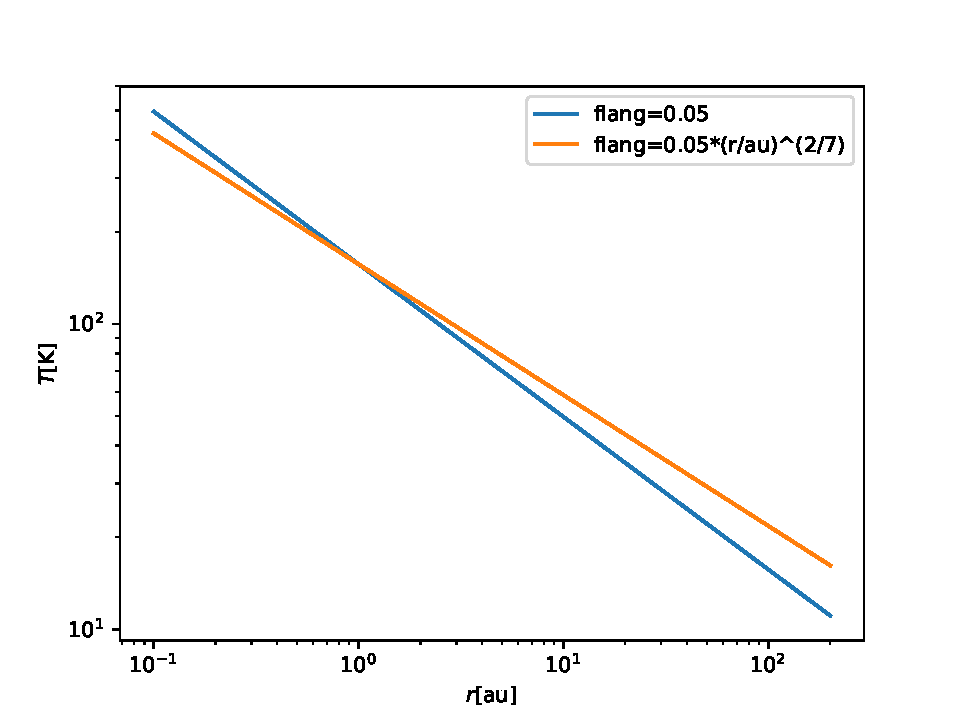
\includegraphics[width=0.7\textwidth]{../snippets/fig_snippet_simple_rt_1_1.pdf}}
To explain what happens here: We make disk models without specifying the surface
density, but we specify the flaring angle $\varphi=0.05$ for the first
model. For the second model we specify a radius-dependent flaring angle
$\varphi(r)=0.05\,(r/\mathrm{au})^{2/7}$. The initialization of the object
automatically calls the \code{compute\_disktmid()} method.  In neither of the
two cases the surface density has to be specified.

A slightly more sophisticated example:
Instead of setting the flaring angle directly, we set the {\em flaring index},
which is the ratio of $\varphi$ to $H_p/r$. This requires iteration, which
quickly converges.
The code snippet is
\code{snippet\_iterate\_hp\_1.py}. In Python run it as:
\begin{codebox}
%run snippet_iterate_hp_1.py
\end{codebox}
Here is the listing:
\lstinputlisting{../snippets/snippet_iterate_hp_1.py}
\centerline{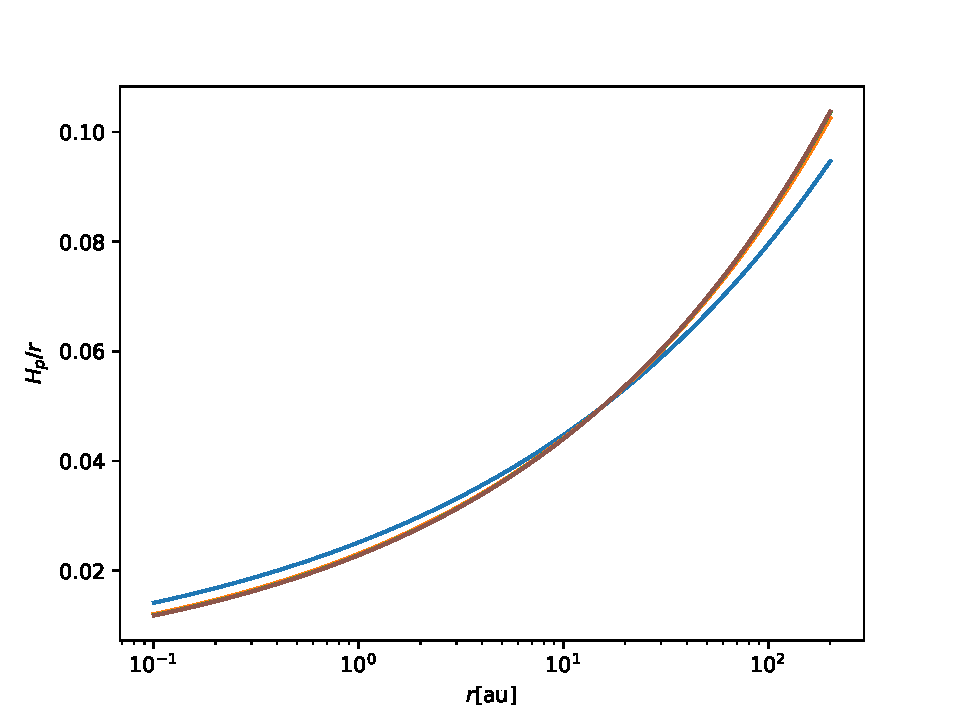
\includegraphics[width=0.7\textwidth]{../snippets/fig_snippet_iterate_hp_1_1.pdf}}
A self-consistent model, however, requires the self-consistent
computation of the surface height $H_s$ (see Chiang \& Goldreich 1997;
Chiang et al.\ 2001; and Dullemond \& Dominik 2001). Then, however, the surface
density of the gas (or more importantly: that of the dust) as well as the dust
opacities are required. See Subsection \ref{sec-disk-flaring} where this is worked out.

So far we have not included the viscous heating into the computation of the midplane
temperature. We refer this to Subsection \ref{sec-viscous-heating}.

\section{Computing the disk mass}
The method \code{compute\_mass()} computes the disk mass in gram,
if the disk is already installed.
\begin{equation}
M_{\mathrm{disk}} = 2\pi \int_{r_{\mathrm{in}}}^{r_{\mathrm{out}}} r \Sigma_g(r) dr
\end{equation}
where the integral is computed as a numerical sum. This value is stored as
\code{mass}. This mass includes only the gas. The disk
mass is automatically computed when one of the standard disk models of
Chapter \ref{chap-standard-disk-models} are set up. But sometimes one
may want to recompute the disk mass. Example:
\begin{codebox}
from disklab.diskradial import *
from disklab.natconst import *
d = DiskRadialModel(rout=500*au,mdisk=0.01*MS)
factor=np.exp(-d.r/(200*AU))
d.sigma *= factor
d.compute_mass()
print('New disk mass = {} Msun'.format(d.mass/MS))
\end{codebox}

\section{Computing the Toomre Q value}
\label{sec-toomre-q}
%
The method \code{compute\_qtoomre()} compute the Toomre Q value for the
gas:
\begin{equation}
Q_g(r) = \frac{c_s\Omega_K}{\pi G \Sigma_g}
\end{equation}
stored as \code{Q}. If a dust component is present, the same will be computed
for the dust and stored in \code{Qdust}, where $c_s$ is then replaced by
$\Omega_K H_d$ with $H_d$ the vertical scale height of the dust layer. Example
for gas:
\begin{codebox}
from disklab.diskradial import *
import matplotlib.pyplot as plt
from disklab.natconst import *
d1=DiskRadialModel(mdisk=0.1*MS,rout=50*au,plsig=-1)
d1.compute_qtoomre()
d2=DiskRadialModel(mdisk=0.1*MS,rout=50*au,plsig=-1.5)
d2.compute_qtoomre()
plt.plot(d1.r/au,d1.qtoomre,label='plsig=-1')
plt.plot(d2.r/au,d2.qtoomre,label='plsig=-1.5')
plt.xscale('log')
plt.yscale('log')
plt.xlabel(r'$r [\mathrm{au}]$')
plt.ylabel(r'$Q$')
plt.show()
\end{codebox}

\section{Computing the deviation from Kepler rotation}
\label{sec-compute-omega}
For most purposes a protoplanetary disk can be considered to be perfectly
Keplerian.  However, when it comes to dust radial drift (see Chapters
\ref{chap-adding-dust-component} and \ref{chap-dust-drift-mixing}) even a small
deviation from Kepler rotation can be important. And when the pressure in the
disk midplane varies too strongly with radius (e.g.\ if one has dense gas rings
or deep disk gaps) then the disk may become unstable and produce Rossby wave
vortices.

So \code{DiskRadialModel} has some routines for computing these things.

The method \code{compute\_omega()} computes the
double-logarithmic derivative of the gas pressure $d\ln p/d\ln r$, where the gas
pressure $p=\rho c_s^2$ is at the midplane. Optionally one can also use the
vertically-integrated gas pressure $P=\Sigma c_s^2$, which is the relevant one
for some 2-D ($r,\phi$) hydrodynamic codes of disks. This option can be selected
by setting \code{vertint=True}. But the default is the gas pressure at the
midplane. This double-logarithmic derivative is stored as \code{dlnpdlnr}.

The $\Omega$ is then computed as
\begin{equation}
\Omega = \Omega_K \sqrt{1+\left(\frac{c_s^2}{v_K^2}\right)\frac{d\ln p}{d\ln r}}
\end{equation}
where $v_K=\Omega_K r$. Furthermore following things are computed and stored:
\begin{eqnarray}
v_\phi &=& \Omega r\\
l_\phi &=& \Omega r^2\\
\delta v_\phi &=& v_\phi - v_K
\end{eqnarray}

Example: let us compute the deviation from Kepler for a Lynden-Bell \& Pringle
model (we will use one of {\sf DISKLAB}'s standard disk models, of Chapter
\ref{chap-standard-disk-models}, the one described in Section
\ref{sec-standard-model-lbp-as-alpha}). The code snippet is\\
\code{snippet\_deviation\_kepler\_1.py}. In Python run it as:
\begin{codebox}
%run snippet_deviation_kepler_1.py
\end{codebox}
Here is the listing:
\lstinputlisting{../snippets/snippet_deviation_kepler_1.py}
\centerline{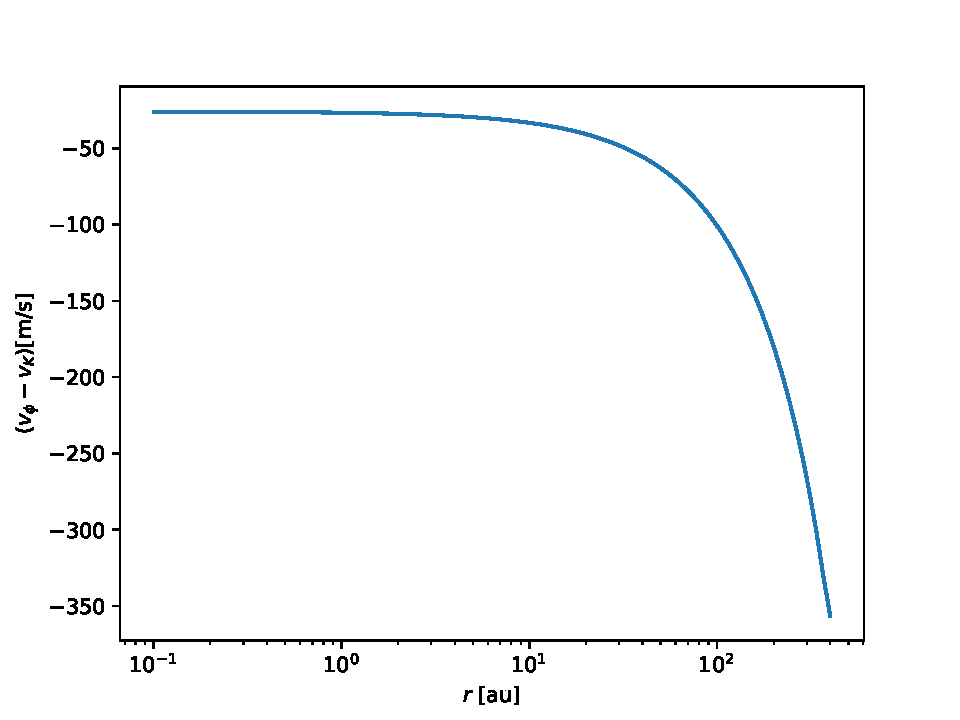
\includegraphics[width=0.7\textwidth]{../snippets/fig_snippet_deviation_kepler_1_1.pdf}}
The various things this method computes are:
\begin{codebox}
d.omega       # Orbital angular frequency [1/s]
d.vphi        # Azimuthal gas velocity [cm/s]
d.dvphi       # Azimuthal gas velocity - Kepler velocity [cm/s]
d.lphi        # Specific angular momentum [cm^2/s]
d.dlnpdlnr    # Double-logarithmic derivative of the pressure
\end{codebox}

\section{Computing the Solberg-Hoiland frequency}
The method \code{compute\_solberg\_hoiland()} computes the value of
the Solberg Hoiland criterion number
\begin{equation}
\mathrm{SH} = \kappa^2 + N^2
\end{equation}
If $\mathrm{SH}>0$ then the disk is stable. If $\mathrm{SH}<0$ then the disk is
Rayleigh unstable. We follow Li, Finn, Lovelace \& Colgate (2000) ApJ 533, 1023,
Equation 22.

The $\kappa$ is given by the derivative of the specific angular momentum in the
following way:
\begin{equation}
\kappa^2 = \frac{1}{r^3}\frac{dl^2}{dr}
\end{equation}

The Brunt-Vaisala frequency is given by:
\begin{equation}
  N^2    = \frac{1}{\rho}\frac{dp}{dr}\left(\frac{1}{\rho}\frac{d\rho}{dr}-
  \frac{1}{\gamma p}\frac{dp}{dr}\right)
\end{equation}
where $\gamma$ is the adiabatic index.

Example where we add a bump to the disk and see if it is stable or not:
The code snippet is
\code{snippet\_deviation\_kepler\_2.py}. In Python run it as:
\begin{codebox}
%run snippet_deviation_kepler_2.py
\end{codebox}
Here is the listing:
\lstinputlisting{../snippets/snippet_deviation_kepler_2.py}
\centerline{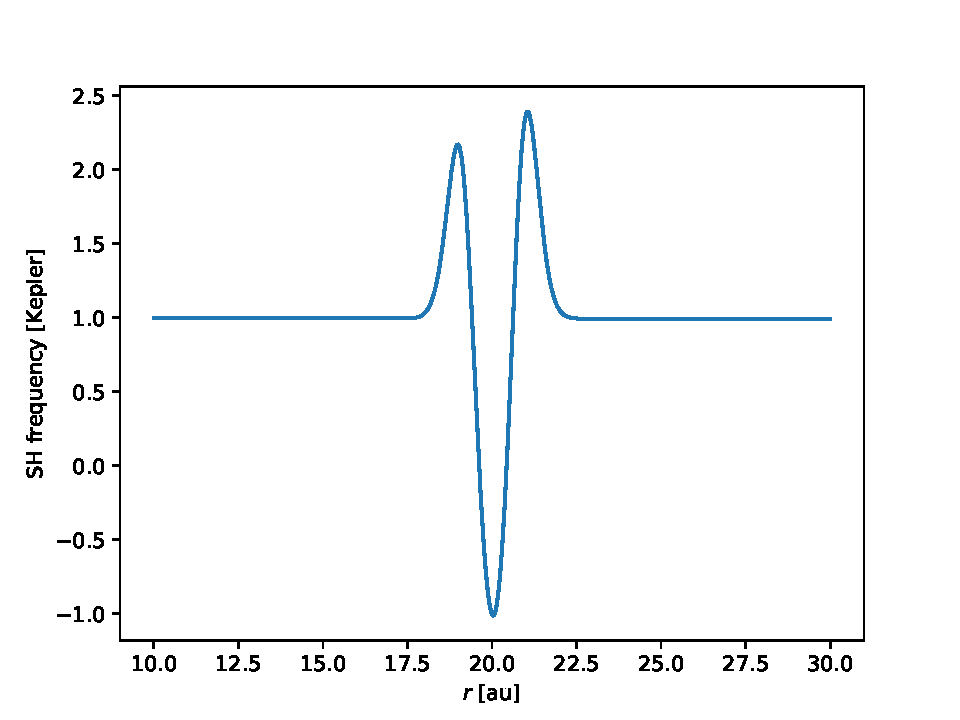
\includegraphics[width=0.7\textwidth]{../snippets/fig_snippet_deviation_kepler_2_1.pdf}}
There where the curve drops below 0 the disk is unstable. This is because the
bump (i.e.~ring) is too narrow.


\section{For convenience: the {\tt DiskRadialModel.plot()} method}\label{sec-disk-standard-plot}
Sometimes it might be useful to be able to plot certain results with a single
command, rather than a series of \code{plt.xxxxx()} commands. The \code{DiskRadialModel.plot()}
method allows you to make standard plots of any content of the \code{DiskRadialModel} object.
Here is an example:
\begin{codebox}
from disklab.diskradial import *
from disklab.natconst import *
d=DiskRadialModel(mdisk=0.01*MS)
d.plot(d.sigma,ylabel=r'$\Sigma [\mathrm{g/cm}^2]$')
\end{codebox}
You can, in fact, plot any kind of stuff, e.g.
\begin{codebox}
d.plot(d.sigma*d.r**2,ylabel=r'$\Sigma\,r^2 [\mathrm{g}]$')
\end{codebox}
There are several keywords that can be set: type \code{d.plot?} for more information.
{\em Note:} This method is just offered for convenience. There is no need to use it
other than convenience. For the rest of this tutorial we will not use it, so that
we can keep as closely to \code{matplotlib} style as possible to not complicate things
unnecessarily.


\chapter{Built-in standard 1-D radial disk model setups}\label{chap-standard-disk-models}
The class \code{DiskRadialModel} has several standard simple disk models that
you can choose from. These are created by the methods with names starting
with \code{make\_disk\_from\_***}. The available models are descibed in the
next subsections. In each of these subsections an example is given. If you
want to make a plot of them: see Section \ref{sec-disk-standard-plot}.
Note that in all the disk models described here you can also adapt the
stellar parameters and grid parameters. Example:
\begin{codebox}
from disklab.diskradial import *
from disklab.natconst import *
d = DiskRadialModel(tstar=1e4,mstar=2.5*MS,lstar=40.*LS,rin=0.5*au,rout=300*AU,nr=1000)
d.make_disk_from_m_pl(mdisk=0.01*MS)
\end{codebox}

\section{Standard 1-D radial disk models}\label{sec-standard-disk-models}
\subsection{Disk model: Powerlaw disk}
The method \code{make\_disk\_from\_powerlaw()} makes a powerlaw disk model
according to the formula:
\begin{equation}\label{eq-diskmodel-powerlaw}
\Sigma_g(r) = \Sigma_0 \left(\frac{r}{r_0}\right)^p
\end{equation}
Example
\begin{codebox}
from disklab.diskradial import *
from disklab.natconst import *
d = DiskRadialModel()
d.make_disk_from_powerlaw(1e2,1*au,-1.5)
\end{codebox}

\subsection{Disk model: Powerlaw disk of given mass}\label{sec-standard-powerlaw}
The method \code{make\_disk\_from\_m\_pl()} makes a powerlaw disk model
according to Eq.~(\ref{eq-diskmodel-powerlaw})
where $\Sigma_0$ is computed such that the total disk mass is the value that
is given as a parameter: \code{mdisk} (in gram).
\begin{codebox}
from disklab.diskradial import *
from disklab.natconst import *
d = DiskRadialModel()
d.make_disk_from_m_pl(mdisk=0.01*MS,plsig=-1.5)
\end{codebox}

\subsection{Disk model: Fixed Toomre Q value}
The method \code{make\_disk\_from\_toomre()} makes a disk model by demanding
that everywhere the Toomre Q value is as given:
\begin{equation}
\Sigma_g(r) = \frac{c_s\Omega_K}{\pi G Q}
\end{equation}
Typically one would want to set $Q=2$, so that you get the maximum surface density
of the disk for marginal gravitational stability:
\begin{codebox}
from disklab.diskradial import *
d = DiskRadialModel()
d.make_disk_from_toomre(2.0)
\end{codebox}

\subsection{Disk model: Constant accretion rate disk}
The method \code{make\_disk\_from\_mdot()} creates a disk model that has
a constant $\dot M$ throughout the grid. The standard viscous disk model is
used, where the accretion rate is given by
\begin{equation}
\dot M = -2\pi r \Sigma_g(r) v_r(r)
\end{equation}
where $v_r$ is the radial velocity. Note that the minus sign is a convention:
it is chosen such that inward motion ($v_r<0$) is, by definition, a positive
accretion rate. Again here: only the gas is accounted for.
The radial velocity in steady state is:
\begin{equation}
v_r = -\frac{3}{2}\frac{\nu(r)}{r}
\end{equation}
so that we obtain
\begin{equation}
\dot M = 3\pi \Sigma_g(r) \nu(r)
\end{equation}
And so the formula for the surface density is then:
\begin{equation}
\Sigma_g(r) = \frac{\dot M}{3\pi\nu}
\end{equation}
The viscosity $\nu$ is given by the standard Shakura \& Sunyaev viscosity recipe:
\begin{equation}\label{eq-ss-alpha-visc}
\nu = \alpha\frac{c_s^2}{\Omega_K}
\end{equation}
where the value of $\alpha$ is the variable \code{alpha} of the object, and
can be given as an array (i.e.~$\alpha=\alpha(r)$) or as a global constant (default
is global constant at value \code{alpha = 0.01}). Example:
\begin{codebox}
from disklab.diskradial import *
from disklab.natconst import *
d = DiskRadialModel()
d.make_disk_from_mdot(mdot=1e-8*MS/year)
\end{codebox}

\subsection{Disk model: Lynden-Bell \& Pringle}
The method \code{make\_disk\_from\_lyndenbellpringle()} sets up
the most famous time-dependent disk model: the analytic solution by
Lynden-Bell \& Pringle.

We follow here the description from the paper Lodato,
Scardoni, Manara \& Testi (2017), MNRAS 472, 4700, their Eqs. 2, 3 and 4.
\begin{equation}
\Sigma_g(r) = \frac{M_0}{2\pi R_0^2}(2-\gamma)\left(\frac{R_0}{r}\right)^\gamma
T^{-\eta}\exp\left(-\frac{(r/R_0)^{(2-\gamma)}}{T}\right)
\end{equation}
with
\begin{eqnarray}
  \nu &=& \nu_0 \left(\frac{r}{R_0}\right)^\gamma\\
  t_\nu &=& \frac{R_0^2}{3(2-\gamma)^2\nu_0}\\
  T &=& 1+\frac{t}{t_\nu}\\
  \eta &=& \frac{2.5-\gamma}{2-\gamma}
\end{eqnarray}
The $R_0$ variable sets the {\em initial} radius of the disk, the $\gamma$ sets
the powerlaw of the viscosity (for a ``normal'' constant $\alpha$ disk this is
$\gamma=1$), and $M_0$ sets the initial disk mass.

A key property of this model setup is that you have to specify the {\em time}
at which you want to have the disk model. This time is the time after $t=0$ of
the Lynden-Bell \& Pringle model. Example
\begin{codebox}
from disklab.diskradial import *
from disklab.natconst import *
d    = DiskRadialModel()
M0   = 1e-2*MS
R0   = 1.0*au
nu0  = 1e10
gam  = 1.0
time = 1e5*year
d.make_disk_from_lyndenbellpringle(M0,R0,nu0,gam,time)
\end{codebox}

\subsection{Disk model: Lynden-Bell \& Pringle as an $\alpha$-disk}
\label{sec-standard-model-lbp-as-alpha}
The method \code{make\_disk\_from\_lbp\_alpha()} sets up a Lynden-Bell \&
Pringle model in which the $\nu$ is according to this $\alpha$-recipe, with
viscosity $\nu$ set according to Eq.~(\ref{eq-ss-alpha-visc}),

{\em Important:} When using this method, the $\alpha$ must be a global constant
or a global powerlaw. The $\gamma$ of the Lynden-Bell \& Pringle model will
be computed as the double-logarithmic numerical derivative
only from the first two grid points:
\begin{equation}
\gamma =\left.\frac{d\ln\nu}{d\ln r}\right|_{r=r_{\mathrm{in}}}
\end{equation}
and $\nu_0$ is obtained from
\begin{equation}
\nu_0 = \nu(r=R_0)
\end{equation}
using numerical interpolation.
\begin{codebox}
from disklab.diskradial import *
from disklab.natconst import *
d    = DiskRadialModel()
M0   = 1e-2*MS
R0   = 1.0*au
alpha= 1e-2
time = 1e5*year
d.make_disk_from_lbp_alpha(M0,R0,alpha,time)
\end{codebox}

\subsection{Disk model: Simplified Lynden-Bell \& Pringle}
The method \code{make\_disk\_from\_simplified\_lbp()} computes a simplified
Lynden-Bell \& Pringle model often used in the literature.
The time-dependent part is removed and only the following formula given:
\begin{equation}
\Sigma_g(r) = \Sigma_c \left(\frac{R_c}{r}\right)^\gamma \exp\left(-\left(\frac{r}{R_c}\right)^{2-\gamma}\right)
\end{equation}
\begin{codebox}
from disklab.diskradial import *
from disklab.natconst import *
d    = DiskRadialModel()
Rc   = 1.0*au
Sigc = 200.
gam  = 1.0
d.make_disk_from_simplified_lbp(Sigc,Rc,gam)
\end{codebox}

\section{Modifying a standard disk model to your wishes}
Standard disk models (such as those from Section \ref{sec-standard-disk-models})
are all nice and good, but {\sf DISKLAB} is meant for you to experiment with
your own models. Usually this means you start with a standard model, and then
modify it to your needs. The nice thing of the \code{DiskRadialModel} class is that
you can modify the disk in any way you like.

\subsection{Modifying a disk model ``by hand''}\label{sec-modif-by-hand}
The simplest form is simply to first create a disk model, and then modify
it by hand. Example:
\begin{codebox}
from disklab.diskradial import *
from disklab.natconst import *
import matplotlib.pyplot as plt
d = DiskRadialModel(mdisk=0.01*MS)
gapr = 10*au
gapw = 2*au
gapd = 0.9
factor = 1. - gapd*np.exp(-0.5*(d.r-gapr)**2/gapw**2)
d.sigma *= factor
d.add_dust(agrain=1e-4)
lam = 0.13
d.compute_onezone_intensity(lam)
plt.plot(d.r/au,d.intensity)
plt.xscale('log')
plt.yscale('log')
plt.show()
\end{codebox}
\noindent where we already used some elements from Section \ref{sec-add-dust} and
Section \ref{sec-simple-radtrans}.

\subsection{Built-in analytic planet gap models}
Although the simple gap model built in by hand in Section \ref{sec-modif-by-hand}
works fine, it can be sometimes useful to implement slightly more sophisticated
planetary gap models. The \code{DiskRadialModel} class has a built-in routine for that,
which contains some models and new models may be added later. Example
\begin{codebox}
from disklab.diskradial import *
from disklab.natconst import *
import matplotlib.pyplot as plt
d = DiskRadialModel(mdisk=0.01*MS,nr=1000)
d.add_dust(agrain=1e-4)
d.add_planet_gap(5*au,'duffell',mpl=2e-4*MS,smooth=2.)
lam = 0.13
d.dust[0].grain.compute_simple_opacity(lam,tabulatemean=False)
d.compute_onezone_intensity(lam)
plt.plot(d.r/au,d.intensity[0,:])
plt.xlim(3,7)
plt.ylim(0,2e-12)
plt.show()
\end{codebox}
This punches a gap into a disk according to the model of Duffell (2015) ApJL
807, 11. To make the gap a bit more smooth (rather than the sudden flat-bottom
gap of Duffell) a smoothing parameter is added.

\chapter{Disk midplane temperature: Irradiation, disk flaring, and viscous dissipation}
\label{sec-irradiation-flaring-viscous-heating}
%
So far we have assumed, for simplicity, that the incidence angle of the stellar
radiation (the flaring angle $\varphi(r)$ stored as \code{d.flang}) is a
constant throughout the disk, and that the midplane temperature is only given by
the irradiation of the disk by the central star (see section
\ref{sec-compute-tmid}). These assumptions made it easy to compute
$T_{\mathrm{mid}}(r)$, by simply using Eq.~(\ref{eq-tmid-from-irradiation}).

However, the assumption that $\varphi(r)$ is a constant is not a very good
assumption. For quick testing purposes it is ok, but for more accurate
calculations it is not recommended. We want to compute it self-consistently.
We follow Chiang \& Goldreich (1997, henceforth CG97) here. The main new
concept we introduce here is the {\em surface height} $H_s(r)$, which is
typically larger than the pressure scale height $H_p(r)$, and represents
the height above the midplane where the disk becomes optically thick to
the stellar radiation.

\section{Computing $H_s(r)$ and $\varphi(r)$ mutually self-consistently}
\label{sec-disk-flaring}
First let us do the exercise of computing $H_s(r)$ and $\varphi(r)$
self-consistently for a fixed $H_p(r)$. That is: we do not treat (for now)
the pressure scale height $H_p(r)$ to be dependent on $\varphi(r)$,
even though it is through the midplane temperature and sound speed.

The flaring angle is, according to CG97, their Eq. 5, given by
\begin{equation}\label{eq-flang-cg}
\varphi(r) = \frac{0.4 R_{*}}{r} + r\frac{d}{dr}\left(\frac{H_s}{r}\right)
\end{equation}
where $H_s$ is the surface height of the disk. The surface height is defined
by the height above the midplane $z=H_s$ where the optical depth with respect
to stellar radiation is unity. Let us compute this height.

Let us first define the dust opacity at stellar wavelength to be $\kappa_{*}$,
and that only the dust produces opacity (not the gas). Let us assume that the
dust and the gas are well mixed, so that the dust-to-gas ratio is the same at
all $z$. Let us call this dust-to-gas ratio $\mathrm{dtg}$. Then the vertical
optical depth to stellar radiation $\tau_{*}$ (without the flaring angle) is
\begin{equation}
\tau_{*} = \mathrm{dtg}\,\Sigma_g\kappa_{*}
\end{equation}
Next we assume that the gas density is vertical distributed according to
the following Gaussian:
\begin{equation}\label{eq-vertstr-gauss}
\rho_g(r,z) = \frac{\Sigma_g(r)}{\sqrt{2\pi}\,H_p}\exp\left(-\frac{z^2}{2H_p^2}\right)
\end{equation}
where $H_p$ is the pressure scale height given by
Eq.~(\ref{eq-pressure-scale-height}). We assume that the dust density
follows the gas density: $\rho_d(r,z)=\mathrm{dtg}\,\rho_g(r,z)$, by virtue
of the assumption of perfect vertical mixing.

Given the irradiation angle $\varphi(r)$, which we assume to {\em not} depend
on $z$, we can compute the optical depth to stellar radiation along the incident
angle as a function of $z$:
\begin{equation}
  \tau_{*,\mathrm{irr}}(r,z) = \frac{\mathrm{dtg}\,\kappa_{*}}{\varphi(r)}
  \int_z^\infty \rho_g(r,z)dz
\end{equation}
We now wish to find the $z$ (for given $r$) at which $\tau_{*,\mathrm{irr}}(r,z)= 1$.
We follow Dullemond \& Dominik (2001), appendix A2, their Eq. A9. In
our form this amounts to solving
\begin{equation}\label{eq-solve-for-hs}
1-\mathrm{erf}\left(\frac{H_s}{\sqrt{2}\,H_p}\right) = \frac{2\varphi}{\tau_{*}}
\end{equation}
for $H_s$.

Now that we have $H_s(r)$ we can integrate Eq.~(\ref{eq-flang-cg}) to obtain
$\varphi(r)$ and then we iterate until convergence. Unfortunately this
procedure is numerically unstable. Chiang et al.~(2001) ApJ 547, 1077
devised a method to keep it stable. Our version of it is to define the
{\em flaring index} $\xi$ as follows:
\begin{equation}\label{eq-flaring-index}
\xi(r) = \frac{d\ln(H_s/r)}{d\ln r}
\end{equation}
so that the {\em flaring angle} (Eq.~\ref{eq-flang-cg}) becomes:
\begin{equation}\label{eq-flang-from-flidx}
\varphi(r) = \frac{0.4 R_{*}}{r} + \xi(r)\frac{H_s}{r}
\end{equation}
The flaring index $\xi(r)$ is now computed in a pairwise fashion,
where gridpoints \code{i} and \code{i+1} store the flaring index
computed from gridpoints \code{i-1} and \code{i-2}. This means
$\xi_{i+1}=\xi_{i}$ for all even \code{i}. The inner two gridpoints
have, by this procedure, no value. We take them to be copies of
the next two. This procedure turns out to converge quickly.

The procedure to compute $H_s$ by solving Eq.~(\ref{eq-solve-for-hs})
is called \code{compute\_hsurf()}. The procedure for computing
the flaring index according to Eq.~(\ref{eq-flaring-index}) (with
the pairwise method) is \code{compute\_flareindex()}. Finally,
the procedure to compute $\varphi(r)$ from $\xi(r)$ according
to Eq.~(\ref{eq-flang-from-flidx}) is called
\code{compute\_flareangle\_from\_flareindex()}. By iterating
these you can obtain the self-consistent flaring geometry.

The code snippet is
\code{snippet\_iterate\_flang\_1.py}. In Python run it as:
\begin{codebox}
%run snippet_iterate_flang_1.py
\end{codebox}
Here is the listing:
\lstinputlisting{../snippets/snippet_iterate_flang_1.py}
\centerline{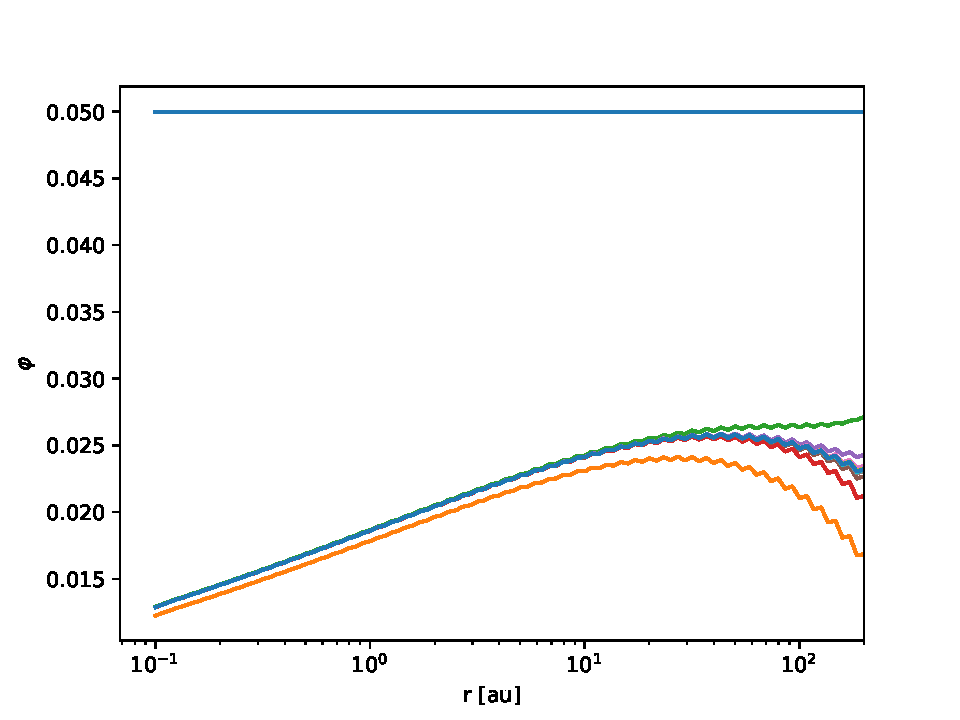
\includegraphics[width=0.7\textwidth]{../snippets/fig_snippet_iterate_flang_1_1.pdf}}

Rather than doing the iteration by hand as above, you can also
use \code{iterate\_flaringangle()}. The code snippet is
\code{snippet\_iterate\_flang\_2.py}. In Python run it as:
\begin{codebox}
%run snippet_iterate_flang_2.py
\end{codebox}
Here is the listing:
\lstinputlisting{../snippets/snippet_iterate_flang_2.py}
\centerline{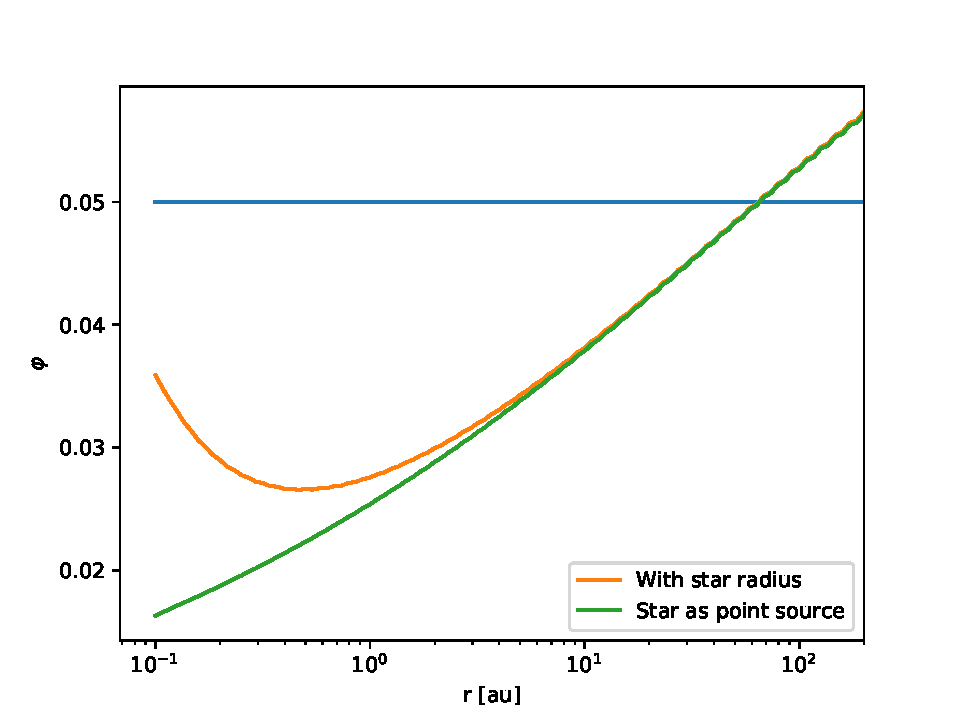
\includegraphics[width=0.7\textwidth]{../snippets/fig_snippet_iterate_flang_2_1.pdf}}
Here we also compare the effect when we include or not include the
$0.4R_{*}/r$ term in Eq.~(\ref{eq-flang-from-flidx}), which is the term
that takes care of the fact that the star is extended (i.e.\ not a point source)
and can thus irradiation even a disk that is not flaring.

Finally, we can now include the self-consistent determination of the
pressure scale height $H_p(r)$ into the iteration, because the flaring angle
determines $T_{\mathrm{mid}}$, which determines $c_s$, which determines
$H_p$. The code snippet is
\code{snippet\_iterate\_flang\_3.py}. In Python run it as:
\begin{codebox}
%run snippet_iterate_flang_3.py
\end{codebox}
Here is the listing:
\lstinputlisting{../snippets/snippet_iterate_flang_3.py}
\centerline{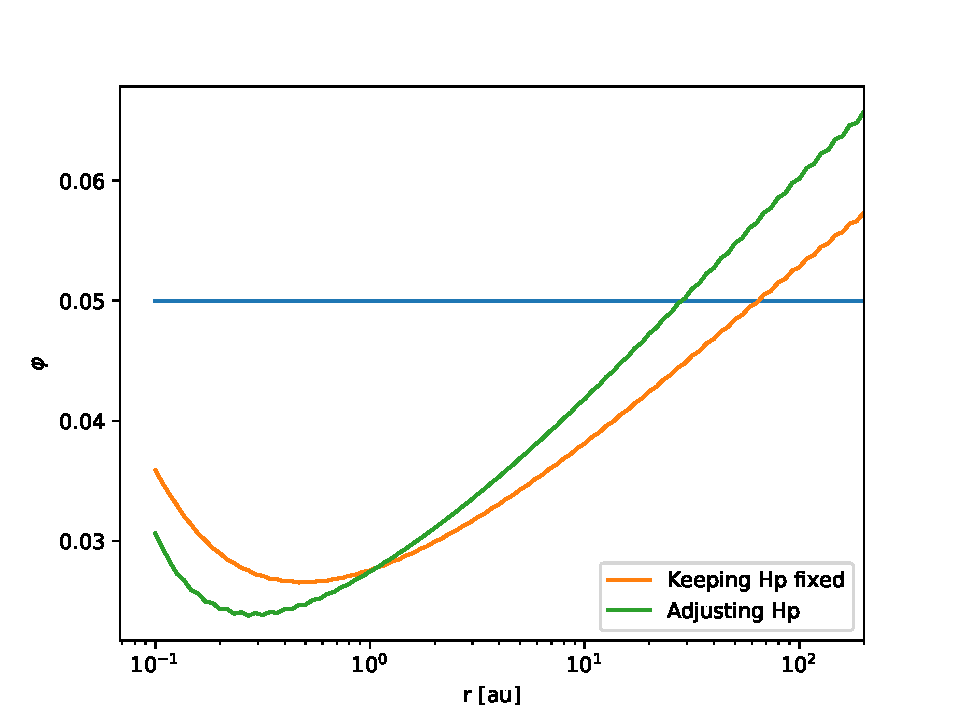
\includegraphics[width=0.7\textwidth]{../snippets/fig_snippet_iterate_flang_3_1.pdf}}
You can also now inspect how the new value of $H_p(r)$ is. This is usually
best done by plotting the ratio $H_p(r)/r$. The code snippet is
\code{snippet\_iterate\_flang\_4.py}. In Python run it as:
\begin{codebox}
%run snippet_iterate_flang_4.py
\end{codebox}
\centerline{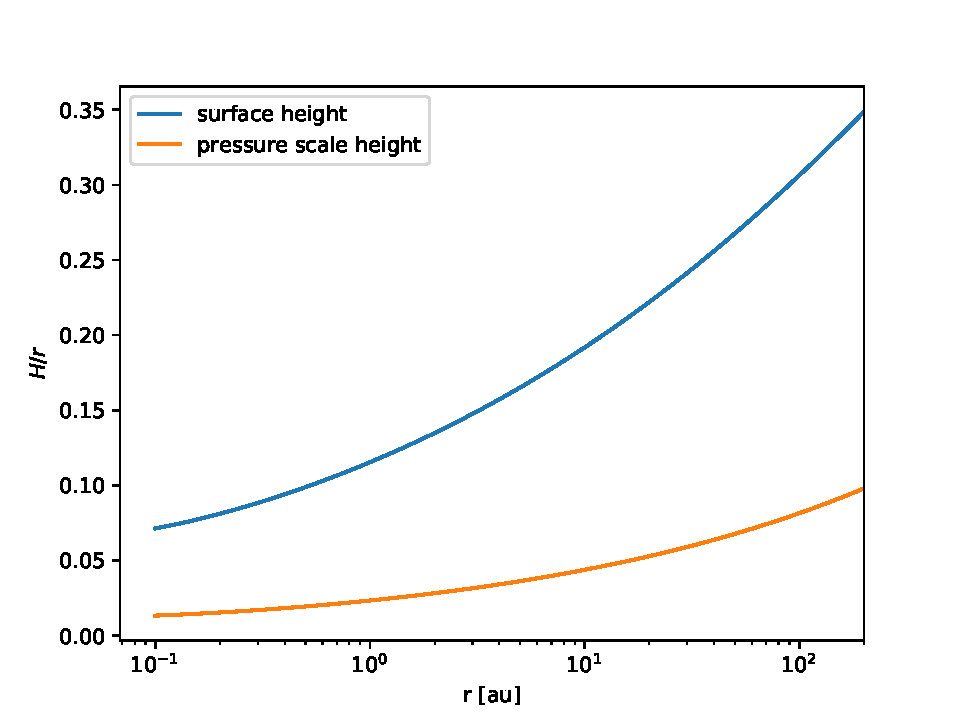
\includegraphics[width=0.7\textwidth]{../snippets/fig_snippet_iterate_flang_4_1.pdf}}

{\bf IMPORTANT:} For disks that are not very optically thick anymore, and/or for
the very outer regions of the disk, the disk is no longer flaring. The disk
becomes {\em self-shadowed}, and thus the above mathematics will fail.  The only
real solution would then be to resort to actual 2-D/3-D radiative transfer,
which is not included in the \code{diskradial} module. It is also important to
keep in mind that the puffed-up inner rim is not included in these calculations,
and also there the only real solution is to resort to 2-D/3-D radiative
transfer. See Section \ref{sec-dust-inner-rim} for some more notes on this.


\section{Including viscous heating in midplane temperature computation}
\label{sec-viscous-heating}
%
In Subsection \ref{sec-compute-tmid} and in Section \ref{sec-disk-flaring}
we compute the midplane temperature from the irradiation by the central
star. However, a viscously accreting disk also produces its own heating.
Including this into the computation of $T_{\mathrm{mid}}(r)$ is both easy
and hard. It is easy because one can easily add a recipe to do that. It
is hard, because (a) it is not really well known at which height in the
disk the heat is deposited and (b) the midplane temperature depends on
the dust opacity. The dust can sublimate if the temperature at the
midplane gets too high, which leads to a kind of ``thermostat effect''.

The viscous heating rate is well-defined:
\begin{equation}
Q_{\mathrm{visc}}(r) = \frac{9}{4}\Sigma_g(r)\nu(r)\Omega_K(r)^2
\end{equation}
The effective temperature at the surface of the disk (assuming the
disk is optically thick) is easily computed, by setting
$Q_{\mathrm{visc}}(r)=Q_{\mathrm{cool}}(r)$, with $Q_{\mathrm{cool}}(r)$ given
by Eq.~(\ref{eq-q-cool-simple}):
\begin{equation}\label{eq-visc-teff-simple}
2\sigma_{\mathrm{SB}}T_{\mathrm{eff}}(r)^4 = \frac{9}{4}\Sigma_g(r)\nu(r)\Omega_K(r)^2
\end{equation}

At this point it becomes important to realize that if the Rosseland mean optical
depth of the disk $\tau_{\mathrm{Ross}}$ becomes lower than about unity,
Eq.~(\ref{eq-visc-teff-simple}) becomes invalid. In such a case one should
replace Eq.~(\ref{eq-q-cool-simple}) with
\begin{equation}\label{eq-q-cool}
  Q_{\mathrm{cool}}(r) = 2 \sigma_{\mathrm{SB}} T_{\mathrm{eff}}(r)^4
  \left(1-e^{-2\tau_{\mathrm{Ross}}}\right)
\end{equation}
where $\tau_{\mathrm{Ross}}$ is the Rosseland optical depth of the disk:
\begin{equation}
\tau_{\mathrm{Ross}} = \Sigma_d \kappa_{d,\mathrm{Ross}}
\end{equation}
where $\kappa_{d,\mathrm{Ross}}$ is the Rosseland opacity of the dust and
$\Sigma_d$ the dust surface density.  The cooling rate formula of
Eq.~(\ref{eq-q-cool}) is approximately valid for any value of
$\tau_{\mathrm{Ross}}$. For $\tau_{\mathrm{Ross}}\gg 1$ it converges to the
familiar Eq.~(\ref{eq-q-cool-simple}). For $\tau_{\mathrm{Ross}}\ll 1$ it
converges to $Q_{\mathrm{cool}}\rightarrow
4\sigma_{\mathrm{SB}}\tau_{\mathrm{Ross}}T_{\mathrm{eff}}^4$, which is the
optically thin cooling rate. With these changes, Eq.~(\ref{eq-visc-teff-simple})
changes to
\begin{equation}\label{eq-visc-teff}
  2\sigma_{\mathrm{SB}}T_{\mathrm{eff}}(r)^4 = \frac{9}{4}\left(1-e^{-2\tau_{\mathrm{Ross}}}\right)^{-1}\Sigma_g(r)\nu(r)\Omega_K(r)^2
\end{equation}

Another difficulty lies in the fact that the midplane temperature is not equal
to the effective temperature. Assuming that all the viscous heat is
deposited at the midplane, the relation between $T_{\mathrm{eff}}$ and
$T_{\mathrm{mid}}$ is
\begin{equation}\label{eq-relation-tmid-teff}
T_{\mathrm{mid}}^4 = \left(\frac{1}{2}\tau_{\mathrm{Ross}}+1\right) T_{\mathrm{eff}}^4
\end{equation}
The factor 1/2 in
Eq.~(\ref{eq-relation-tmid-teff}) comes in because $\tau_{\mathrm{Ross}}$ is the
{\em total} vertical optical depth, while we need the optical depth from the
midplane to the surface. The $+1$ inside the brackets of
Eq.~(\ref{eq-relation-tmid-teff}) is a approximation to keep the equation also
valid for $\tau_{\mathrm{Ross}}\ll 2$.

In principle Eqs.~(\ref{eq-visc-teff}) and (\ref{eq-relation-tmid-teff})
complete the formula for the midplane temperature:
\begin{equation}\label{eq-visc-tmid}
  2\sigma_{\mathrm{SB}}T_{\mathrm{mid}}(r)^4 = \frac{9}{4}\left(\tfrac{1}{2}\tau_{\mathrm{Ross}}+1\right)
  \left(1-e^{-2\tau_{\mathrm{Ross}}}\right)^{-1}
  \Sigma_g(r)\nu(r)\Omega_K(r)^2
\end{equation}
Although it seems that Eq.~(\ref{eq-visc-tmid}) gives the final answer,
there are several loose ends:
\begin{enumerate}
\item\label{point-nudepend-iteration} The value of $\nu(r)$ depends on the midplane temperature itself
  (Eq.~\ref{eq-ss-alpha-visc}). This means iteration is required.
\item The Rosseland opacity $\kappa_{d,\mathrm{Ross}}(r)$ also depends on the
  midplane temperature, because it is the Rosseland-average at the temperature
  of the infrared radiation inside the disk. It is certainly not the same as the
  $\kappa$ we used in Section \ref{sec-disk-flaring} for computing the flaring
  angle (which is the opacity at stellar wavelengths).
\item To do it right, one should spatially resolve the disk vertically, because
  the temperature is a gradial function of vertical coordinate $z$. But usually
  this is ignored for simplicity.
\item\label{point-combine-visc-irr} Usually {\em both} viscous heating and irradiation take place. The
  formula Eq.~(\ref{eq-visc-tmid}) only treats the viscous heating.
\item The viscous heating can lead to the inner disk regions becoming
  {\em self-shadowed}. This means that the irradiation by the central
  star of this region is zero. In reality it is, however, not exactly
  zero because the disk surface is not infinitely geometrically thin.
  Also radial radiative diffusion will transport heat into this region,
  but treating this requires full 2-D/3-D radiative transfer.
\end{enumerate}

Concerning point \ref{point-nudepend-iteration}: In principle one could solve
Eq.~(\ref{eq-visc-tmid}) in the simplest possible iterative way: keep
$\tau_{\mathrm{Ross}}$ and $\nu$ from the previous iteration, and evaluate
the right-hand-side of Eq.~(\ref{eq-visc-tmid}), thus obtaining
$T_{\mathrm{mid}}$, and then re-evaluate $\tau_{\mathrm{Ross}}$ and $\nu$
for this new $T_{\mathrm{mid}}$ and repeat the process until convergence.
This is the solution method used when you call \code{compute\_disktmid()}
with the keyword \code{simple=True}. But this simple iteration can fail,
in particular if dust sublimation is included in the mean opacity model.

Instead, by default the \code{compute\_disktmid()} method uses Brent's
root-finding
algorithm\footnote{\url{https://en.wikipedia.org/wiki/Brent's_method}}
to solve for $T_{\mathrm{mid}}$. This is a much more robust method.

Concerning point \ref{point-combine-visc-irr}: combining viscous heating and irradiation.
There is no unique way, because in reality one would have to resolve the
vertical structure. We do this here in the following way: we compute
the midplane temperature due to iraddiation-only and call this $T_{\mathrm{irrad}}$,
and compute the midplane temperature due to viscous-heating-only and call
this $T_{\mathrm{visc}}$. Then we combine them in the following way:
\begin{equation}
T_{\mathrm{mid}} = \left(T_{\mathrm{irrad}}^4 + T_{\mathrm{visc}}^4 \right)^{1/4}
\end{equation}
Let's compute this in an example. The code snippet is
\code{snippet\_tmid\_viscousheating\_1.py}. In Python run it as:
\begin{codebox}
%run snippet_tmid_viscousheating_1.py
\end{codebox}
Here is the listing:
\lstinputlisting{../snippets/snippet_tmid_viscousheating_1.py}
\centerline{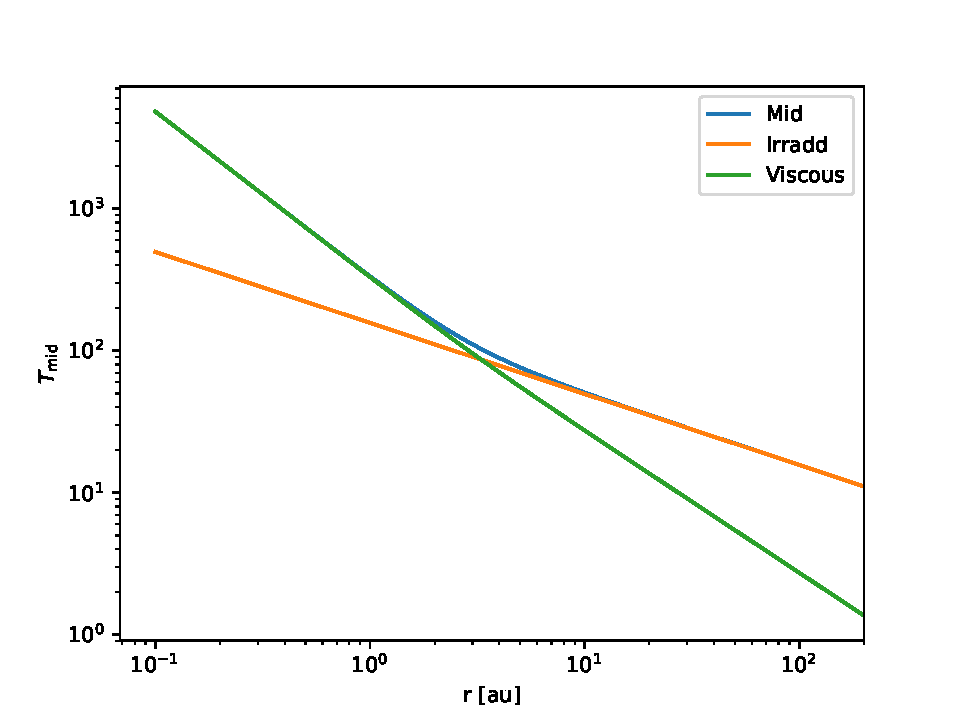
\includegraphics[width=0.7\textwidth]{../snippets/fig_snippet_tmid_viscousheating_1_1.pdf}}
Note that here we kept the flaring angle fixed at $\varphi(r)=0.05$.

If we re-compute the flaring angle after the inclusion of the viscous heating,
we will encounter the effect of self-shadowing in the viscously heated part of
the disk. Since self-shadowing can not be properly modeled using the flaring
angle recipe, it can lead to somewhat odd behavior of the result. In the
following example such behavior of the model is shown. The code snippet is
\code{snippet\_tmid\_viscousheating\_2.py}. In Python run it as:
\begin{codebox}
%run snippet_tmid_viscousheating_2.py
\end{codebox}
Here is the listing:
\lstinputlisting{../snippets/snippet_tmid_viscousheating_2.py}
\centerline{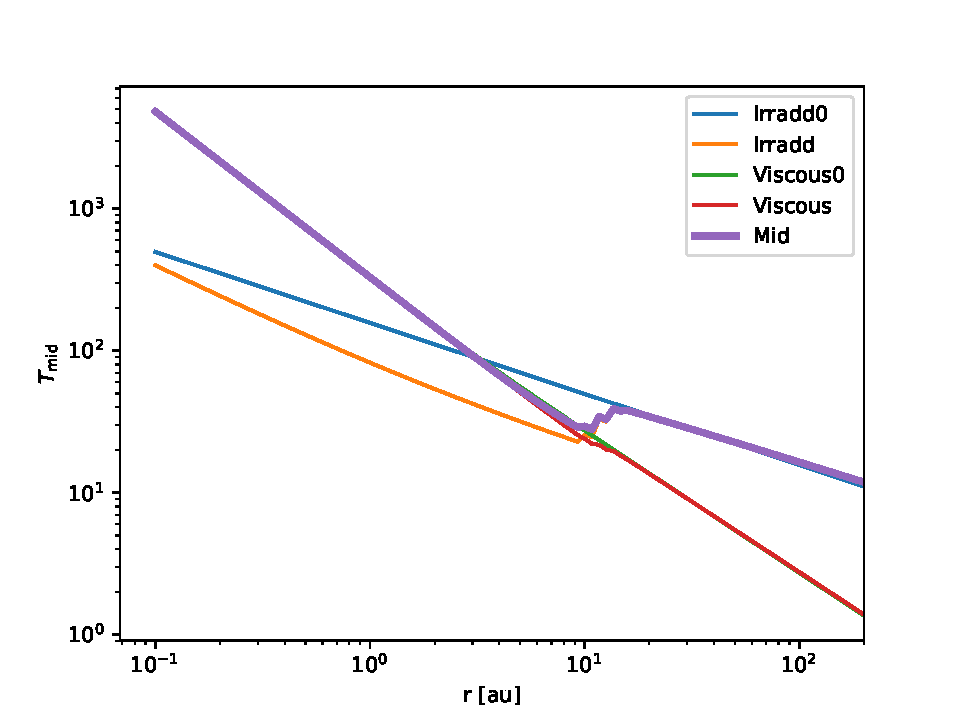
\includegraphics[width=0.7\textwidth]{../snippets/fig_snippet_tmid_viscousheating_2_1.pdf}}
Until about 10 au the disk midplane is dominated by the viscous heating
(compare the ``Irrad'' curve to the ``Viscous'' curve: the latter being much
larger than the former). This make the disk more ``conical'' in shape, and
thus aggravates the effect of the reduced contribution of the irradiation:
The disk wants to become self-shadowed here. Beyond 10 au, however, the
irradiation dominates over the viscous heating, making the disk strongly
flaring, which increases the flaring angle, and thus reinforces the effect.
The dramatic step in temperature around 10 au is likely an artifact of the
iteration of the flaring angle recipe in part of the disk that ``wants'' to
become self-shadowed. In reality the jump is not expected to be so strong.
But a proper treatment requires 2D/3D radiative transfer.

Before concluding this section, let us go back to the previous simple
case, but now replace the supersimple opacity with a more realistic opacity:
the Bell \& Lin opacity model (see Section \ref{sec-mean-opac-bellin}).

The code snippet is
\code{snippet\_tmid\_viscousheating\_3.py}. In Python run it as:
\begin{codebox}
%run snippet_tmid_viscousheating_3.py
\end{codebox}
Here is the listing:
\lstinputlisting{../snippets/snippet_tmid_viscousheating_3.py}
\centerline{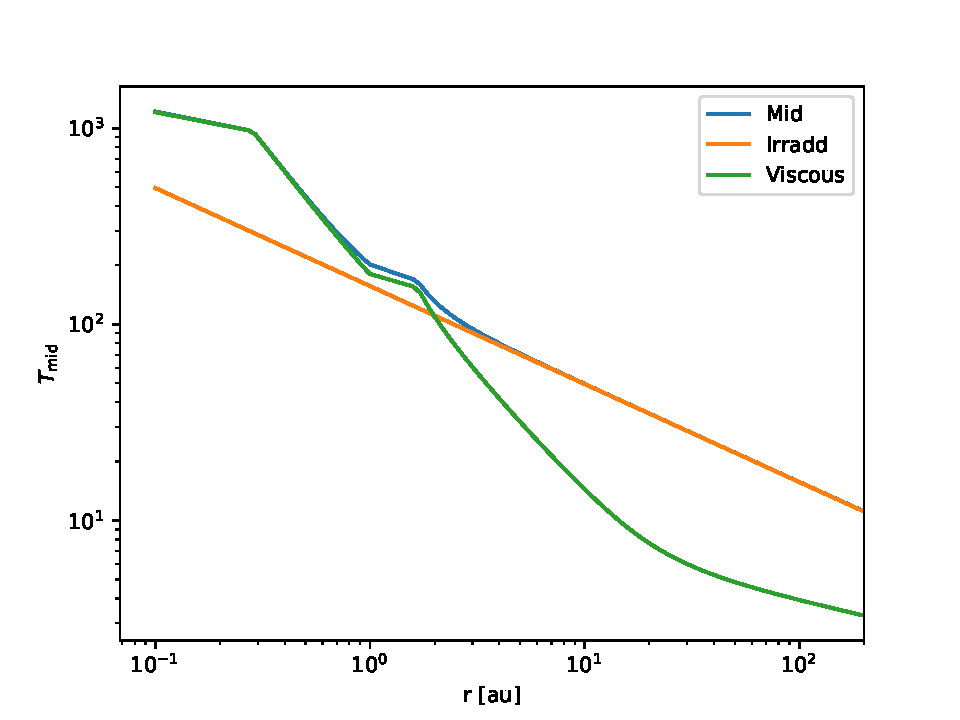
\includegraphics[width=0.7\textwidth]{../snippets/fig_snippet_tmid_viscousheating_3_1.pdf}}
Compared to the \code{snippet\_tmid\_viscousheating\_1.py} case,
which had a smooth transition from irradiated (in the outer region) to
viscous (inner region), we now see several kinks in the temperature
profile. The temperature seems to nearly level off to constant within
two regions. These are the ice line (outer leveled-off region, between about
1 and 2 au) and the dust sublimation line (inner leveled-off region,
inward of about 0.3 au). This leveling off
is a kind of ``thermostat effect'' when the ice or dust starts to
sublimate. In the Bell \& Lin opacity model the sublimation of ice
and silicates occur gradually over an extended range in temperature
(see the figure showing the Bell \& Lin opacity model
of Section.~\ref{sec-opacity-models}), whereas in the opacity model
used in \code{snippet\_viscdiskevol\_4.py} (Section \ref{sec-time-dep-visc-disk})
the sublimation occurs at exactly a single temperature (leading to the
exactly leveled temperature profiles in that model). Reality
probably lies in between these two extremes: At higher densities the sublimation
temperature is at somewhat higher temperature.


\section{Some cautionary comments about the midplane temperature}
\label{sec-midplane-temp-comments}
%
As you can see, the computation of the midplane temperature in a self-consistent
manner is not quite easy. The self-consistent computation of the flaring angle
is not always really possible, because the flaring-angle-recipe itself may break
down due to multi-dimensional radiative transfer effects. To include such
multi-dimensional radiative transfer effects you either have to resort to
full-scale radiative transfer codes such as \code{RADMC-3D} (see e.g.~Chapter
\ref{chap-links-to-external-codes}), or to simplified 2-D radiative diffusion-based
methods such as described in Section \ref{sec-fld-rt-model} in the Chapter on
vertical structure models (Chapter \ref{chap-vertical-structure}).

Also the viscous heating may not be well understood: Is the heat deposited
always near the midplane (proportional to the density) or is it deposited higher
up in the disk?  And what is the effect of thermal sublimation of dust on the
midplane temperature?

And will the environment affect the temperature? Surely the temperature should
not be allowed to drop below the 2.73 microwave background temperature. But given
that stars form in star formation regions, the cumulative radiation from the
nearby young stars will likely provide a higher background temperature. It may
therefore be necessary to set a lower limit to the disk temperature you compute
from the above simple estimates, in particular for very large disks that tend to
become very cold in the outer regions. By default, {\sf DISKLAB} uses
a background temperature of $T_{\mathrm{bg}}=2.725$, i.e.\ the cosmic
microwave background temperature. But you can set this to a higher value
if the protoplanetary disk object resides in a cluster of stars. The best
is to specify this at the very start by setting the \code{tbg} keyword
in your call to \code{DiskRadialModel}. For instance:
\begin{codebox}
d = DiskRadialModel(mstar=2*MS,lstar=10*LS,rin=0.1*au,rout=1000*au,nr=300,tbg=20.)
\end{codebox}
Please keep in mind the simplicity of this method. A more self-consistent radiative
transfer computation can be done with codes such as \code{RADMC-3D} (see e.g.~Chapter
\ref{chap-links-to-external-codes}).

Another potential problem with the determination of the midplane temperature
can emerge when we combine viscous heating with time-dependent viscous
evolution (see Section \ref{sec-numstab-vischeat-opac-evol}). It often
works out of the box, but sometimes, when the opacity model is complex
(e.g.\ has dust evaporation jumps), it can become numerically unstable.
To solve this, please refer to Section \ref{sec-numstab-vischeat-opac-evol}.

\section{A note on constant aspect ratio models}
In many papers on the hydrodynamics of planet-disk interaction and/or
magnetohydrodynamic disk behavior a set of standard assumptions are made that
will make the comparison to the models of {\sf DISKLAB} a bit difficult.

First, these models often assume that the disk has a ``constant aspect ratio''
of, say, 0.05. This is another way of saying that, by assumption,
$h_p/r=0.05$. This means that the midplane disk temperature as a function of
radius is $T(r)=(\mu m_p/k_{\mathrm{B}})(0.05)^2v_K^2(r)\propto r^{-1}$. This is
a steeper temperature profile than we find in the above sections, at least for
the irradiation-dominated part of the disk. The irradiation-dominated disks have
a flaring geometry, i.e.\ $d(h_p/r)/dr>0$, i.e.~a less steep temperature decline
with radius. If the disk is viscous-heating dominated, the opposite can be the
case. If you wish to make {\sf DISKLAB} models that can be compared to
constant aspect ratio models from the literature, you can impose this by
hand, for instance like this:
\begin{codebox}
hr      = 0.05                # Choice of aspect ratio h_p/r
d.cs    = hr*d.r*d.omk
d.hp    = d.cs/d.omk
d.tmid  = 2.3*mp*d.cs**2/kk   # 2.3 is the mean molecular weight
\end{codebox}

Second, these hydrodynamics models are often expressed in ``code units''.
In constrast, {\sf DISKLAB} does not use code units: everything is in real
units (CGS). Any comparison requires a proper conversion.



\chapter{Time-dependent viscous disk evolution}

\section{Time-dependent viscous disk}
\label{sec-time-dep-visc-disk}
The method \code{get\_viscous\_evolution\_next\_timestep()} allows the disk
model to be viscously advanced in time by a single time step $\Delta t$. This
time-advancement is done using an {\em implicit integration method}, and thus is
stable for any value of $\Delta t$. But of course it is better (more accurate)
to do several small time steps than one huge time step. Experimentation may be
required.

The time-dependent viscous disk equation is:
\begin{equation}\label{eq-timedep-viscousdisk}
  \frac{\partial\Sigma_g}{\partial t} + \frac{1}{r}\frac{\partial}{\partial r}
  \left(r\Sigma_g v_r\right) = \dot\Sigma_g
\end{equation}
where $\dot\Sigma_g$ is a possible source term (e.g.\ infall of gas from an
envelope, see Section \ref{sec-time-dep-visc-disk-shu-ulrich}).
Also a negative source term (e.g.\ photoevaporation) is possible,
but that could easily lead to negative surface densities, which would then
also mess up the mass conservation.
The radial velocity due to the viscosity is:
\begin{equation}\label{eq-viscdisk-vr}
v_r = -\frac{3}{\sqrt{r}\,\Sigma_g}\frac{\partial (\sqrt{r}\,\Sigma_g\nu)}{\partial r}
\end{equation}
where $\nu$ is the viscosity coefficient given by Eq.~(\ref{eq-ss-alpha-visc}),
but the viscosity could have any shape. If we insert Eq.~(\ref{eq-viscdisk-vr}) into
Eq.~(\ref{eq-timedep-viscousdisk}) we obtain
\begin{equation}
  \frac{\partial\Sigma_g}{\partial t} - \frac{3}{r}\frac{\partial}{\partial r}
  \left(\sqrt{r}\,\frac{\partial (\sqrt{r}\,\Sigma_g\nu)}{\partial r}\right) = \dot\Sigma_g
\end{equation}

We can now resort to a general-purpose Python subroutine {\small\tt
  solvediffonedee} for solving (or advancing in time) a standard diffusion
equation. This method is described in appendix
\ref{sec-standard-diff-eq-solver-onedee}.

The viscous disk equation Eq.~(\ref{eq-timedep-viscousdisk}) can be cast into
the standard form of Eq.~(\ref{eq-standard-advection-diffusion}), so that we can
use the subroutine \code{solvediffonedee} to advance the viscous
disk in time.

If define $\sigma = 2\pi \Sigma_g r$ and $\dot\sigma = 2\pi \dot\Sigma_g r$ we obtain:
\begin{equation}
  \frac{\partial \sigma}{\partial t} -3\frac{\partial}{\partial r}
  \left(\sqrt{r}\frac{\partial}{\partial r}\left(\sigma\frac{\nu}{\sqrt{r}}\right)\right)=\dot \sigma
\end{equation}
Next define $g(r)=\sqrt{r}/\nu$:
\begin{equation}
  \frac{\partial \sigma}{\partial t} -3\frac{\partial}{\partial r}
  \left(\nu\, g\,\frac{\partial}{\partial r}\left(\frac{\sigma}{g}\right)\right)=\dot\sigma
\end{equation}
Next define $D=3\nu$:
\begin{equation}
  \frac{\partial \sigma}{\partial t} -\frac{\partial}{\partial r}
  \left(D\, g\,\frac{\partial}{\partial r}\left(\frac{\sigma}{g}\right)\right)=\dot\sigma
\end{equation}
This means that we can now use the standard diffusion solver with $y=\sigma$ and $x=r$.

For completeness: the radial velocity is:
\begin{equation}
  v_r = -\frac{3}{\Sigma \sqrt{r}}\frac{\partial}{\partial r}\left(\sqrt{r}\Sigma\nu\right)
  =-\frac{D}{\sigma}g\,\frac{\partial}{\partial r}\left(\frac{\sigma}{g}\right)
\end{equation}
The accretion rate is then:
\begin{equation}\label{eq-mdot-from-sigma-g}
  \dot M(r,t) = -\sigma v_r = D g\,\frac{\partial}{\partial r}\left(\frac{\sigma}{g}\right)
\end{equation}

Example: we set up an initial disk model and let it evolve in time. The code snippet is
\code{snippet\_viscdiskevol\_1.py}. In Python run it as:
\begin{codebox}
%run snippet_viscdiskevol_1.py
\end{codebox}
Here is the listing:
\lstinputlisting{../snippets/snippet_viscdiskevol_1.py}
\centerline{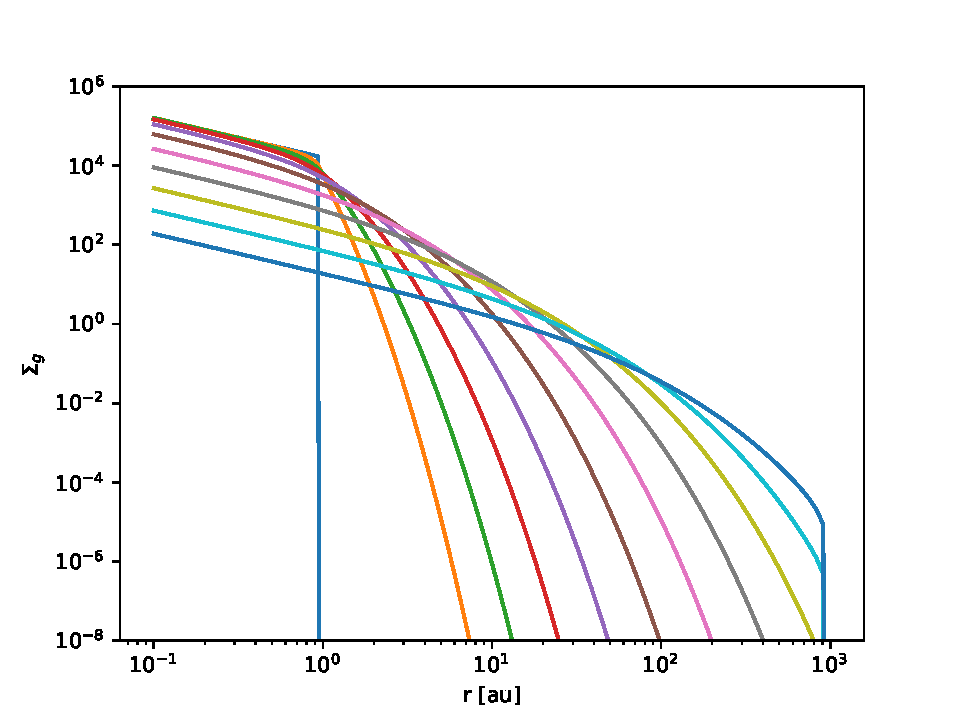
\includegraphics[width=0.7\textwidth]{../snippets/fig_snippet_viscdiskevol_1_1.pdf}}
The different lines are different time snapshots, with logarithmic time intervals.

Ten time steps, logarithmic in time, as shown here is a very coarse time-resolution.
Let us check how the time step size affects the final result (here taken at 3 Myr).
The code snippet is
\code{snippet\_viscdiskevol\_2.py}. In Python run it as:
\begin{codebox}
%run snippet_viscdiskevol_2.py
\end{codebox}
Here is the listing:
\lstinputlisting{../snippets/snippet_viscdiskevol_2.py}
\centerline{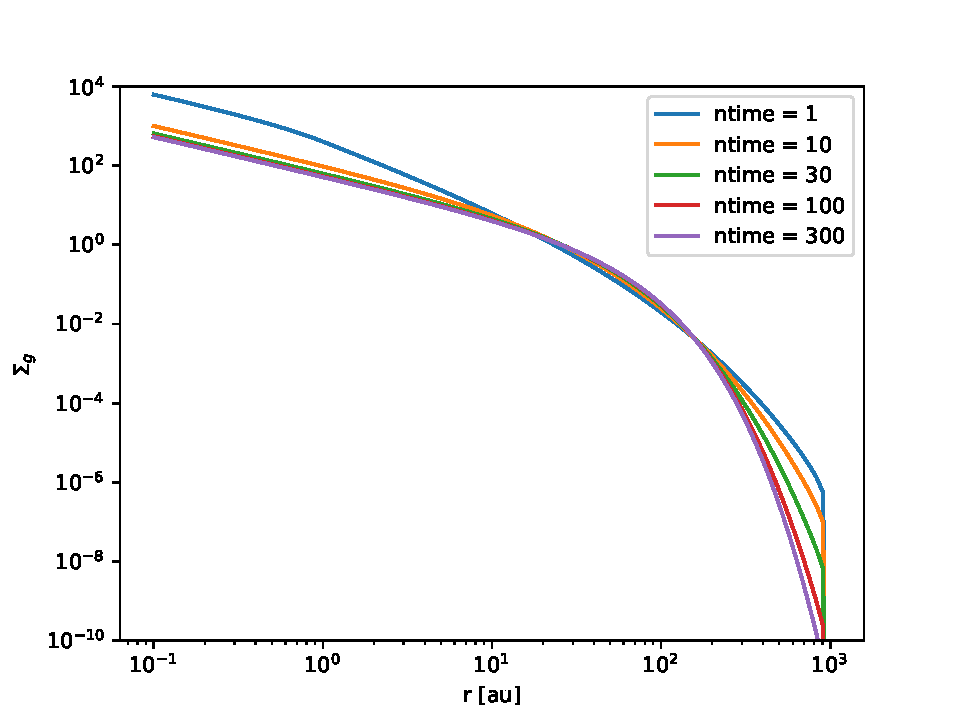
\includegraphics[width=0.7\textwidth]{../snippets/fig_snippet_viscdiskevol_2_1.pdf}}

Comparison to Lynden-Bell \& Pringle solution.
The code snippet is
\code{snippet\_viscdiskevol\_3.py}. In Python run it as:
\begin{codebox}
%run snippet_viscdiskevol_3.py
\end{codebox}
Here is the listing:
\lstinputlisting{../snippets/snippet_viscdiskevol_3.py}
\centerline{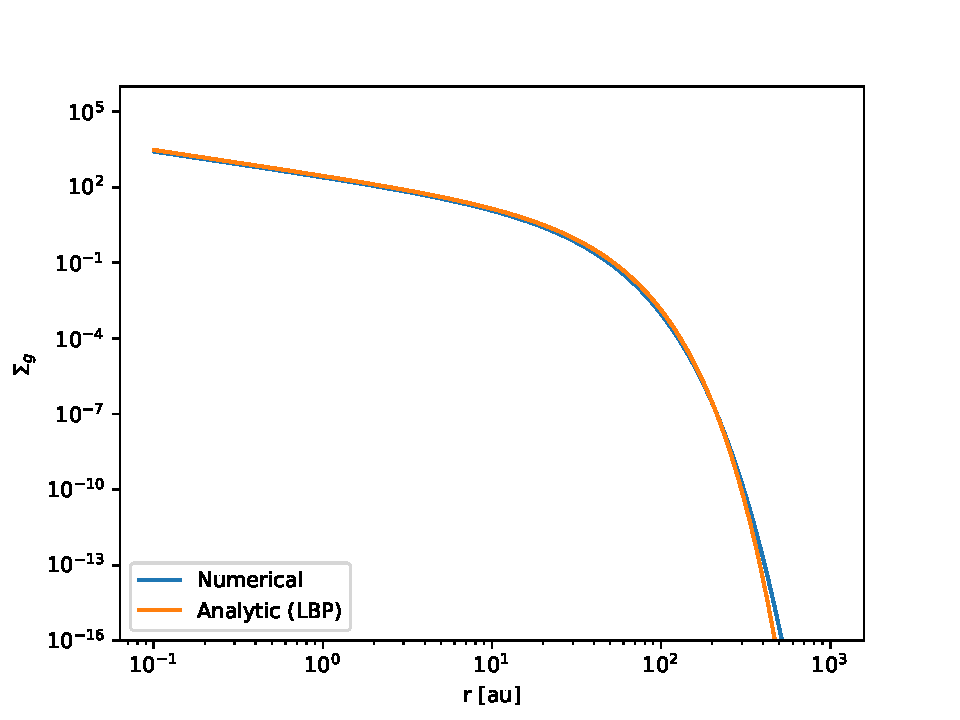
\includegraphics[width=0.7\textwidth]{../snippets/fig_snippet_viscdiskevol_3_1.pdf}}

It is important to note that \code{get\_viscous\_evolution\_next\_timestep()}
only returns the gas surface density $\Sigma_g(r)$. The midplane density is not
updated, unless you explicitly do so by calling
\code{d.compute\_rhomid\_from\_sigma()} after te surface density update.
Another approach is to use the \code{compute\_viscous\_evolution\_next\_timestep()}
method (note: \code{compute} instead of \code{get}), which computes the
surface density $\Sigma_g$ and automatically stores it into \code{d.sigma},
and also recomputes \code{d.rhomid} from that. Simply replace the time loop in
the above snippet(s) by:
\begin{codebox}
for itime in range(1,ntime):
   d.compute_viscous_evolution_next_timestep(time[itime]-time[itime-1])
\end{codebox}

As a slightly more sophisticated example of a viscous accretion model
we update the midplane temperature at every time step using
\code{compute\_disktmid(vischeat=True)}, i.e.\ with the viscous
heating included. To mimick the thermostat effect due to the
dust sublimation we simply limit the temperature by hand to $<$1500 K.
We should in principle also check if the disk becomes superadiabatic
(in which case convection would set in and limit the temperature
further), but in this example we will not do this.

The code snippet is
\code{snippet\_viscdiskevol\_4.py}. In Python run it as:
\begin{codebox}
%run snippet_viscdiskevol_4.py
\end{codebox}
Here is the listing:
\lstinputlisting{../snippets/snippet_viscdiskevol_4.py}
\centerline{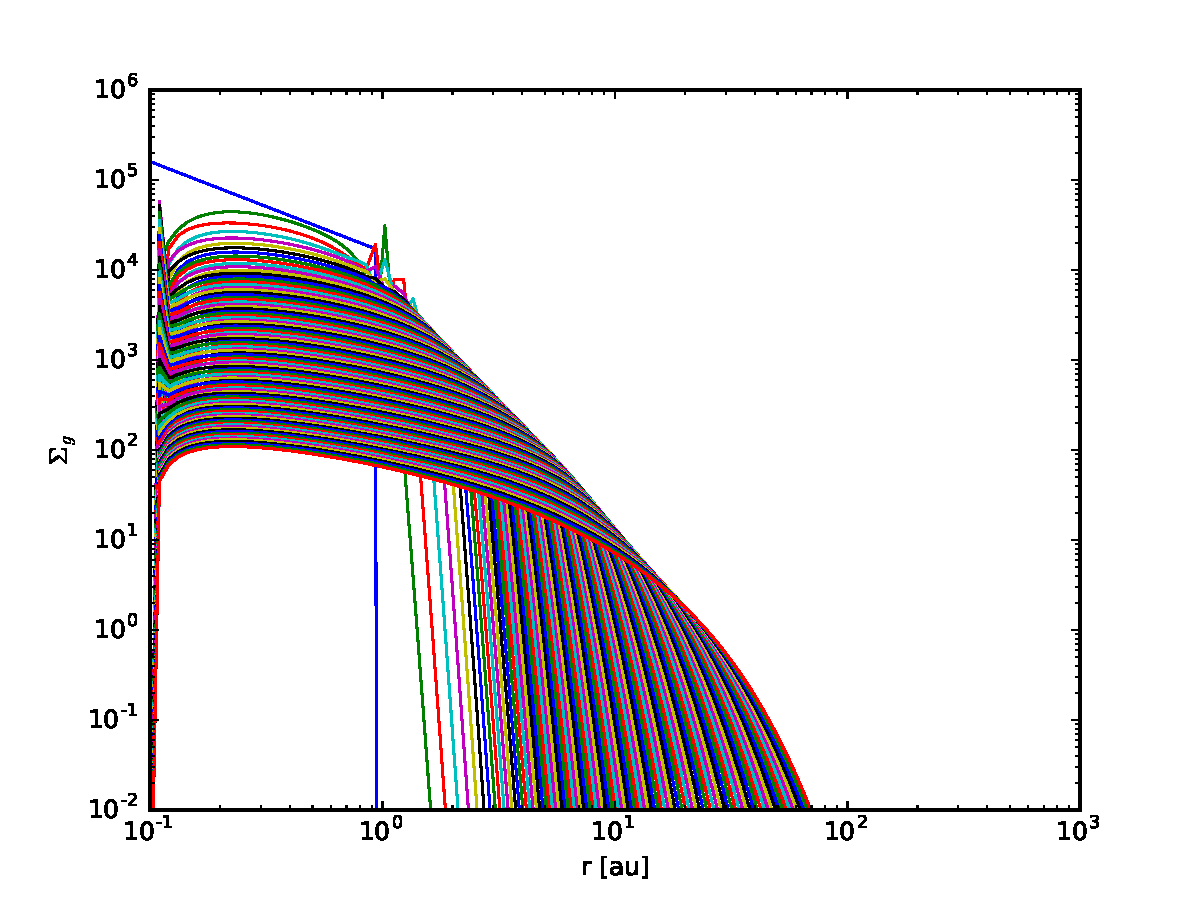
\includegraphics[width=0.45\textwidth]{../snippets/fig_snippet_viscdiskevol_4_1.pdf}
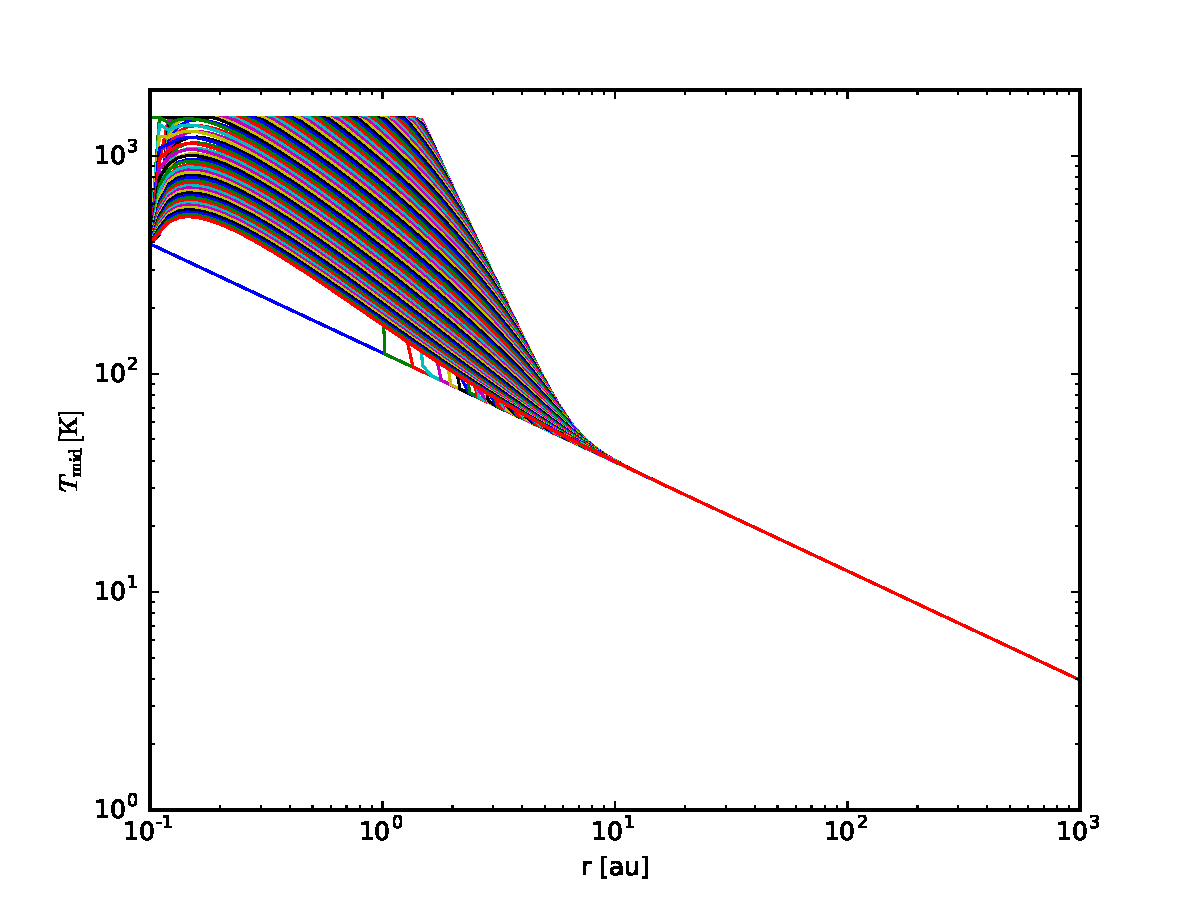
\includegraphics[width=0.45\textwidth]{../snippets/fig_snippet_viscdiskevol_4_2.pdf}}

One can see that initially the temperature near the inner edge saturates
at 1500 K. As time progresses the temperature drops. The numerical wiggles
early on are because the initial disk was taken to have an abrupt outer
edge. As the disk becomes smoother this problem disappears.

{\em Important:} In this example we set the inner boundary condition in a
different way than before: we fixed the surface density to some arbitrary low
value. This is necessary because the default self-adjusting boundary condition
causes an instability for this example. The fixed inner boundary is set using
the keyword \code{sigma\_innerbc}.



\section{Computation of $\dot M$ and $v_r$ for viscous accretion}
\label{sec-comp-mdot-vr}
Whether or not one uses the time-dependent viscous disk integration capability
or not, it can sometimes be useful to compute the accretion rate $\dot M(r)$
and/or the radial velocity of the gas $v_r(r)$ of the disk model. In principle
one could use the formula Eq.~(\ref{eq-viscdisk-vr}) for the radial velocity. But
sometimes it is important to know the values of $\dot M(r)$ and/or $v_r(r)$
exactly, i.e.\ numerically consistent with the time-dependent evolution from
Section \ref{sec-time-dep-visc-disk}. This is necessary, for instance, when
computing the radial transport of dust in the disk: a small numerical mismatch
could jeopardize the dust-to-gas ratio.

So in \code{DiskRadialModel} these values are computed directly from the same
algorithm that advances the disk in time. Note that this also works fine if the
model is not evolved in time. The computation of $\dot M$ and $v_r$ are consistent
with, but not dependent on, the time-evolution method.

The method \code{compute\_mdot\_at\_interfaces()} essentially uses
Eq.~(\ref{eq-mdot-from-sigma-g}), where the derivative is computed numerically
exactly in the same way as in the implicit time evolution.

The method \code{compute\_vr\_at\_interfaces()} first calls the
\code{compute\_mdot\_at\_interfaces()} method to compute $\dot M$ at the
interfaces. Then it divides by $-2\pi r \Sigma_r$ to obtain $v_r$. One can
choose which value of $-2\pi r \Sigma_r$ to take: the average of the values
in the two bordering cells, or the upwind value. This is important if you
use $v_r$ elsewhere for e.g. the advection of a dust species: if you use
upwinding for that, you should also use the upwind method here (which is,
in fact, anyway the default).

Note that both methods return the values {\em at the interfaces}, not at the
cell centers.

The code snippet is
\code{snippet\_compute\_vr\_mdot\_1.py}. In Python run it as:
\begin{codebox}
%run snippet_compute_vr_mdot_1.py
\end{codebox}
Here is the listing:
\lstinputlisting{../snippets/snippet_compute_vr_mdot_1.py}
\centerline{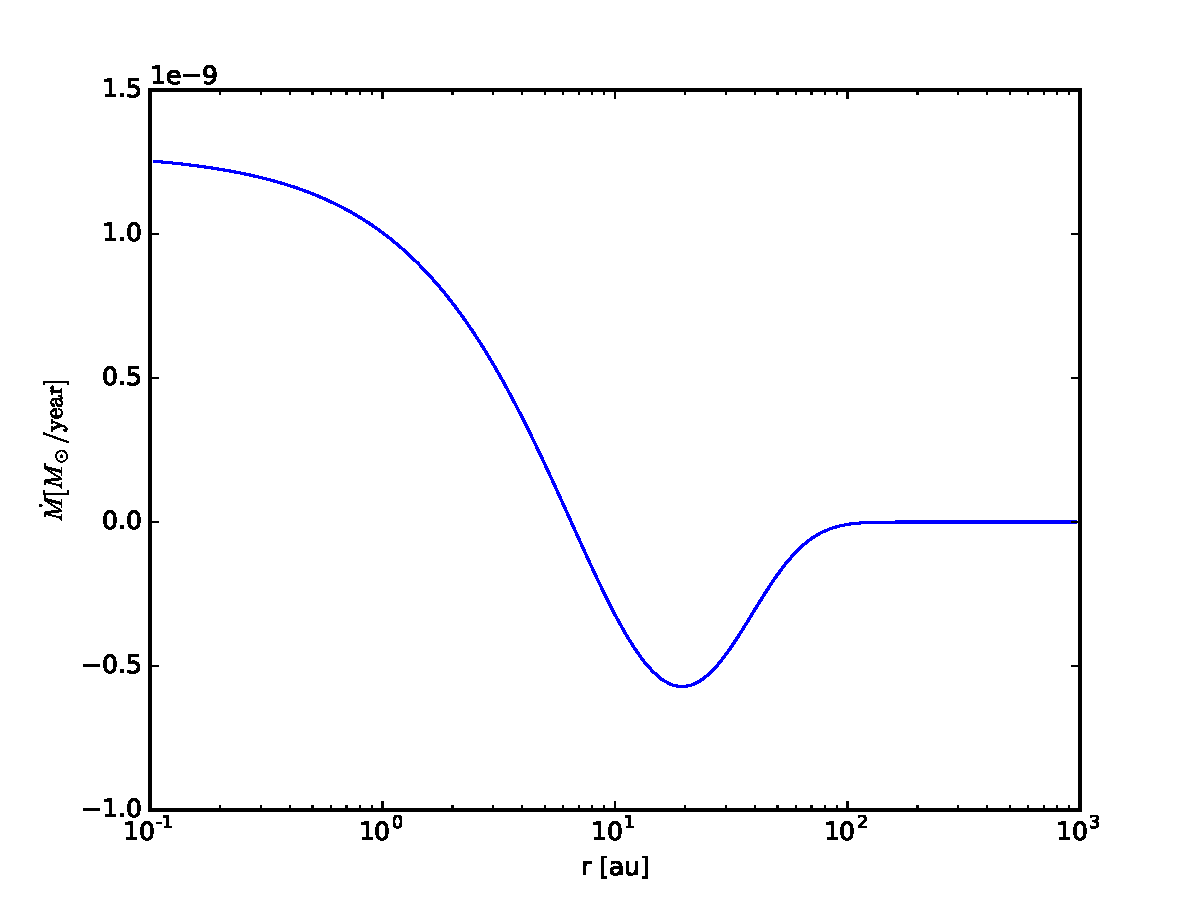
\includegraphics[width=0.5\textwidth]{../snippets/fig_snippet_compute_vr_mdot_1_1.pdf}
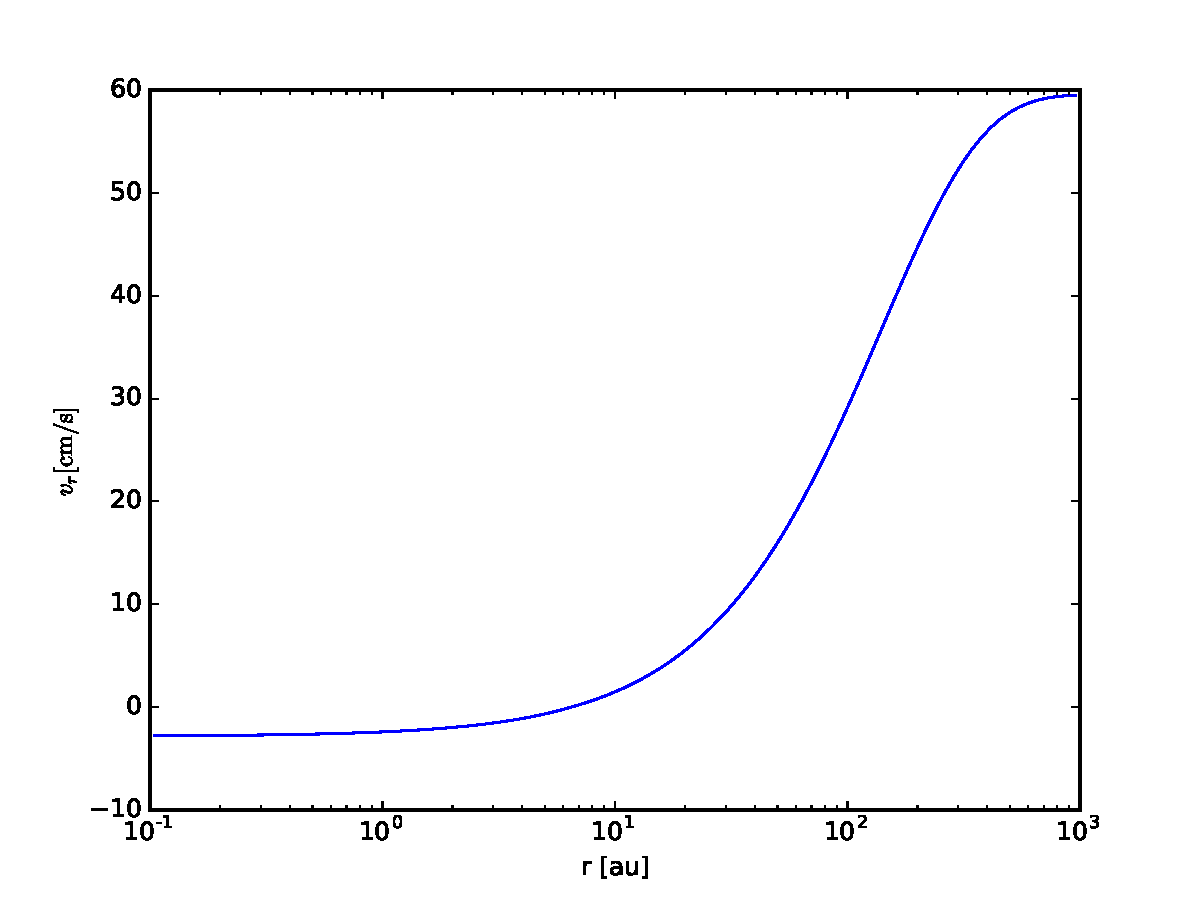
\includegraphics[width=0.5\textwidth]{../snippets/fig_snippet_compute_vr_mdot_1_2.pdf}}
You can see that in the inner disk (inward of about 7 au) the gas flows inward and
the accretion rate is positive (as expected). Beyond about 7 au the gas flows outward,
which is because it absorbs the angular momentum from the inner disk and thus expands
the outer disk. The accretion rate is there negative (outflowing). At very large
radii the $\dot M$ is going back to 0, because there is no material at those
radii.


\section{How to handle gravitational instability}
\label{sec-grav-instab}
%
Under certain conditions a protoplanetary disk can become so massive, that the
Toomre $Q$ parameter (Section \ref{sec-toomre-q}) becomes smaller than 2. This
is in particular to be expected when the disk is still being fed by an infalling
envelope (see Section \ref{sec-time-dep-visc-disk-shu-ulrich}). If this happens,
a gravitational instability (GI) sets in. It is impossible to model the
evolution of the disk when such an instability operates. The GI produces
non-axially symmetric waves in the disk (spiral waves) that strongly
redistribute mass and angular momentum. Since the models in {\sf DISKLAB} are
axially symmetric, a proper treatment of GI is impossible.

It has been suggested in the literature (e.g.~Armitage, Livio \& Pringle 2001,
MNRAS 324, 705) that the GI can be mimicked by an artificially enlarged
$\alpha$-parameter in the region where $Q<2$. Experiments with this method
using {\sf DISKLAB} have yielded violently unstable solutions for the time
step sizes we usually employ.

In {\sf DISKLAB} we therefore use a different method to mimick the effect of
GI. The idea is that we assume that GI will always try to redistribute the mass
in the disk in such a way as to keep $Q\ge 2$: i.e.\ keeping the disk at
marginal stability. We assume that this happens on a time scale faster than the
usual viscous time scale of the disk, i.e.\ basically instantly.

The \code{DiskRadialModel} class of {\sf DISKLAB} therefore offers a method
called \code{gravinstab\_flattening()}. It instantly redistributes the gas
surface density in the disk whereever $Q<2$, such that $Q\ge 2$ is restored
everywhere. The $Q<2$ region thus becomes a $Q=2$ region.  The redistributed
mass is dumped on the inside and outside edges of the $Q<2$ (now $Q=2$) region
in such a way as to increase the local surface density to its maximum, leading
to $Q=2$ there as well. This essentially enlarges the $Q=2$ region. This
redistribution is done in a way as to ensure mass conservation and angular
momentum conservation. The enlarging of the $Q=2$ region on the inside and
outside of the original $Q<2$ region by the dumping of mass is, under the
assumption of mass and angular momentum conservation, uniquely defined.

When calling \code{gravinstab\_flattening()} if the disk has $Q>2$ everywhere,
nothing happens. But if there is a region with $Q<2$, the
\code{gravinstab\_flattening()} method will fix the $Q<2$ issue by generating
instead a region with $Q=2$. This region has an abrupt inner and outer edge,
meaning that the surface density will also have a jump at the inner and outer
edge of the $Q=2$ region. This is not a very realistic effect, but in practice
even a small $\alpha$-viscosity will smooth these edges out a bit.

Note that if the disk has a dust component (see Chapter
\ref{chap-adding-dust-component}), the redistribution of the gas somehow also
has to drag the dust along with it. It would be unphysical to have strong
redistribution of gas, while leaving the dust untouched. After applying
\code{gravinstab\_flattening()} to the gas surface density, you can apply
\code{gravinstab\_apply\_flattening()} to each dust component, to assure that
the dust moves along with the gas during the redistribution.

The idea of using \code{gravinstab\_flattening()} is to apply it (if necessary)
at each time step of a viscous evolution model. Whenever the model tends to
push $Q$ below 2, the \code{gravinstab\_flattening()} will push it back to 2.
In Section \ref{sec-time-dep-visc-disk-shu-ulrich} an example of this is
given.

Here we show an extreme example of a disk that is ``flattened''. 
The code snippet is
\code{snippet\_gravinst\_flattening\_1.py}. In Python run it as:
\begin{codebox}
%run snippet_gravinst_flattening_1.py
\end{codebox}
\centerline{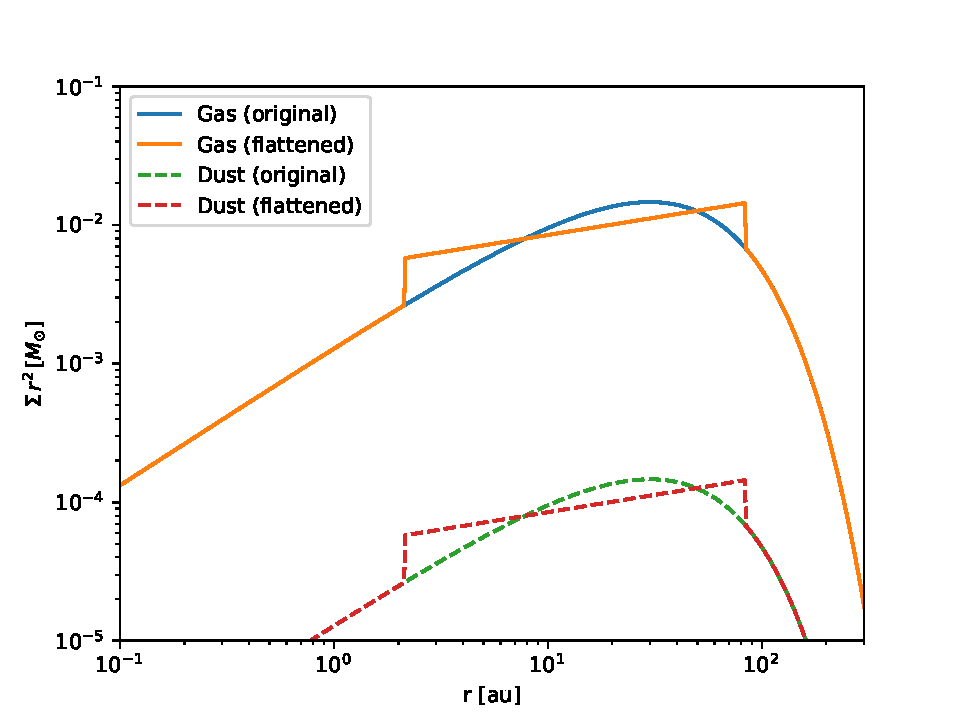
\includegraphics[width=0.5\textwidth]{../snippets/fig_snippet_gravinst_flattening_1_1.pdf}
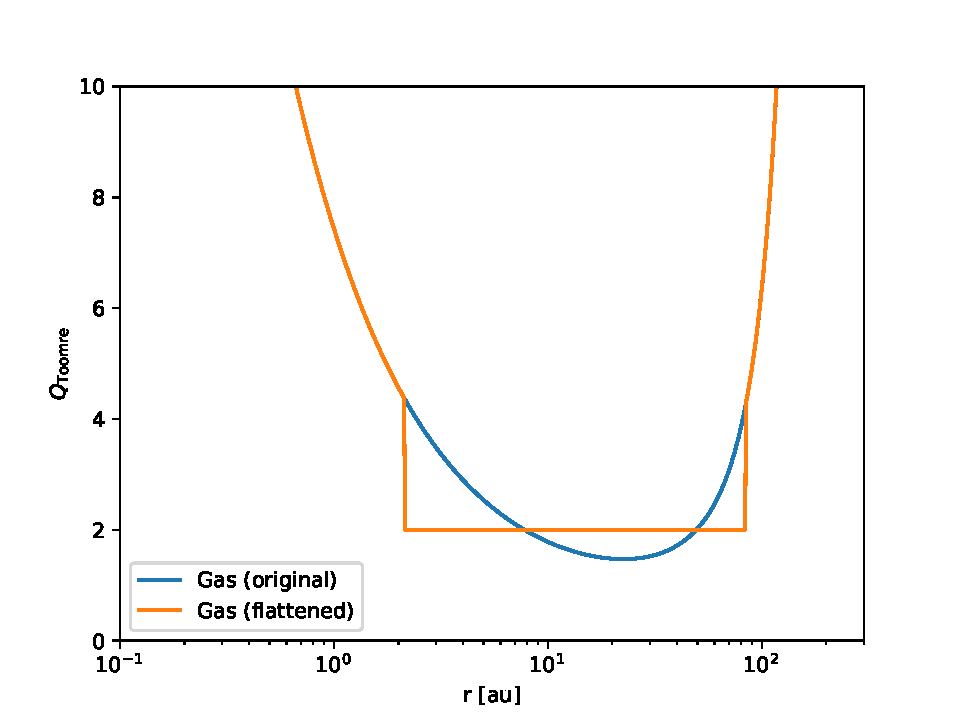
\includegraphics[width=0.5\textwidth]{../snippets/fig_snippet_gravinst_flattening_1_2.pdf}}
Please keep in mind that this example is extreme in the sense that it starts
with a disk that has a region well below $Q=2$, leading to a drastic redistribution
of mass. If the method \code{gravinstab\_flattening()} is applied every time step,
then each such call only redistributes mass moderately.

It can happen that, as a result of the flattening, a lot of mass is collected in
the very innermost radial zone. This is, of course, unphysical. The mass at the
inner zone should be added to the star. To enforce this, you can set the keyword
\code{flushgridedges=True} in the call to \code{gravinstab\_flattening()}. Note
that this option also removes any excessive mass from the outermost zone. But if
mass is accumulated in the outermost zone, it is better to extend the radial
grid outward.

It should be kept in mind that the instant redistribution of mass by the GI is a
pretty strong assumption that may not be correct. If mass loading onto the disk
(see Section \ref{sec-time-dep-visc-disk-shu-ulrich}) is too excessive, the disk
will likely fragment into clumps rather than spread. However, within the context
of {\sf DISKLAB} this is, of course, not possible to model. Also the GI-induced
spiral shock waves will heat the disk. This is, so far, not included in the model.


\section{Viscous disk evolution with Shu-Ulrich infall}
\label{sec-time-dep-visc-disk-shu-ulrich}
%
A protoplanetary disk does not simply get born in its final state. It gets built-up
due to the collapse of a molecular cloud core. This is a complex process that is
presumably not well represented by a simple model. But it is nevertheless very
instructive to include this build-up phase into the viscous disk evolution.

We follow for most part the paper by Hueso \& Guillot (2005) A\&A 442, 703, and
the implementation by Dullemond, Natta \& Testi 2006 A\&A 645, 69 and Dullemond,
Apai \& Walch 2006 A\&A 640, 67. The infall model is that of Shu (1977) ApJ 214,
488, and Ulrich (1976) ApJ 210, 377. These two models are combined where the Shu
model treats the radial infall, while the Ulrich model handles the effect of the
rotation. Without the rotation the disk would not form, so the Ulrich part is
the essential part that creates the disk.

The way we implement the infall is to calculate, at every time step, the
$\dot\Sigma_g(r,t)$ in Eq.~\ref{eq-timedep-viscousdisk}, which is the infall
from the cloud. We do not treat the 3-D effects such as infall onto the outer
edge of the disk.

The computation of $\dot\Sigma_g(r,t)$ is done by the method
\code{compute\_shuulrich\_infall()}.

Let us run such a model. We will reproduce the ``Example 1'' model of
Hueso \& Guillot (2005), were we get the parameters from their Table 4.
The plot of star- and disk-mass as a function of time is their Fig.~5.

The code snippet is
\code{snippet\_infall\_1.py}. In Python run it as:
\begin{codebox}
%run snippet_infall_1.py
\end{codebox}
Here is the listing:
\lstinputlisting{../snippets/snippet_infall_1.py}
Note that this listing has a lot of additional infrastructure to make
useful plots. The actual ``bare'' code that performs the
Hueso\&Guillot-like infall and viscous evolution is only the part inside the time loop.\\
\centerline{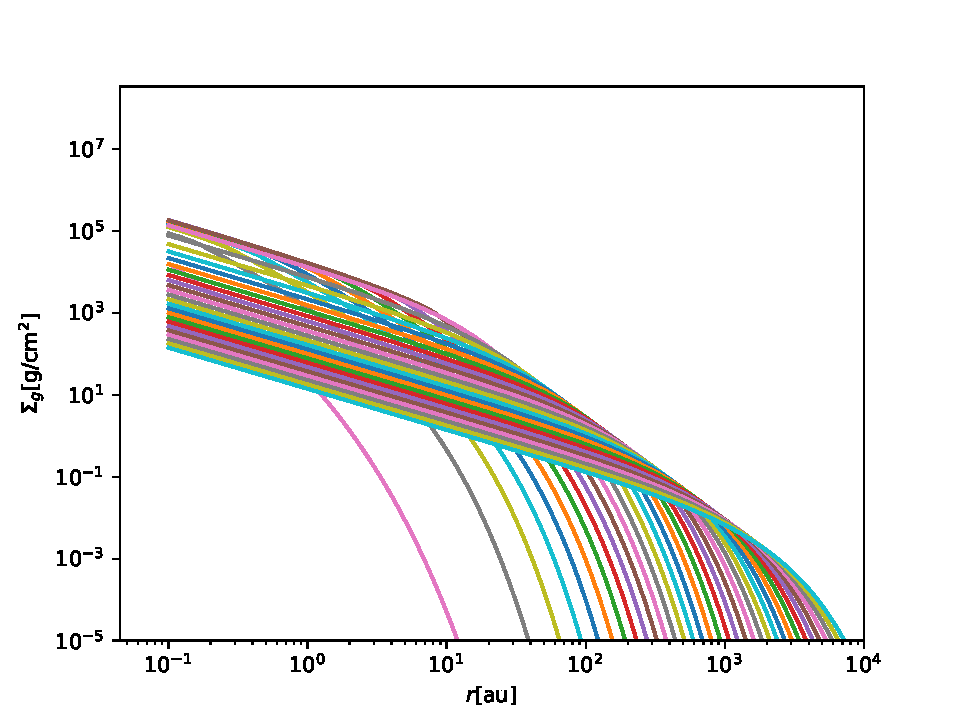
\includegraphics[width=0.5\textwidth]{../snippets/fig_snippet_infall_1_1.pdf}
  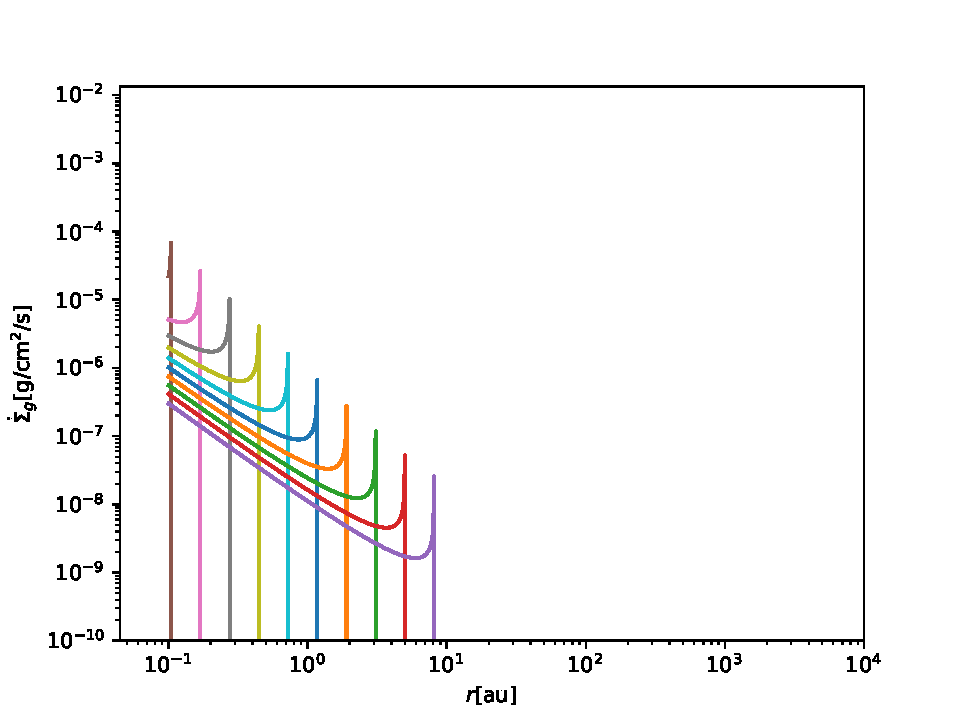
\includegraphics[width=0.5\textwidth]{../snippets/fig_snippet_infall_1_2.pdf}}
Left is the surface density profile $\Sigma_g(r,t)$ for various time snapshots. Right the
$\dot\Sigma_g(r,t)$.\\
\centerline{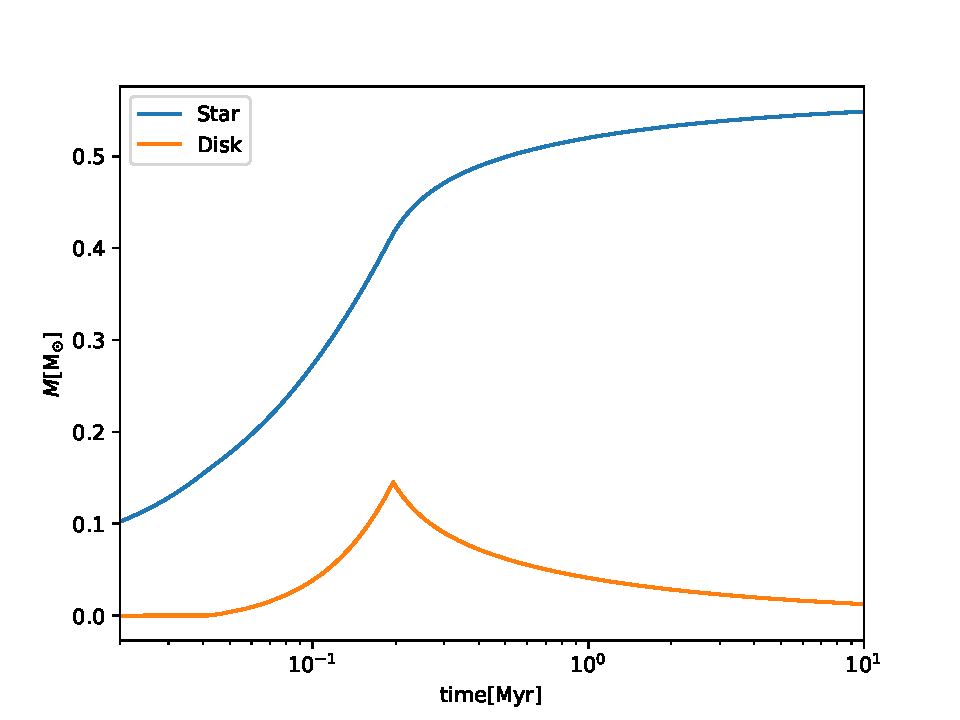
\includegraphics[width=0.7\textwidth]{../snippets/fig_snippet_infall_1_3.pdf}}
The time evolution of stellar and disk mass. Comparing this plot to Hueso \&
Guillot's Fig.\ 5 we see that the match is reasonable. There are some slight
differences, but they are minor. For instance, in their plot the disk only
starts gaining mass after 0.09 Myr, while in our case this happens already at
0.04 Myr because that is about the time when the centrifugal radius of the
infalling material reaches the inner edge of the grid at 0.1 au.  We find that
mass conservation (where the final stellar + disk mass equals the initial
stellar + disk + cloud mass) requires that the first time steps are fairly
small. But since we use, as usual, logarithmically spaced time steps, that is
not a problem. We find 99\% mass conservation.

You can also add a dust component to the infalling gas. A simple example is
to have only 1 grain size of 10 $\mu$m radius with a dust-to-gas ratio of 0.01.
The code snippet is
\code{snippet\_infall\_2.py}. In Python run it as:
\begin{codebox}
%run snippet_infall_2.py
\end{codebox}
The star, disk and dust mass as a function of time is shown here:\\
\centerline{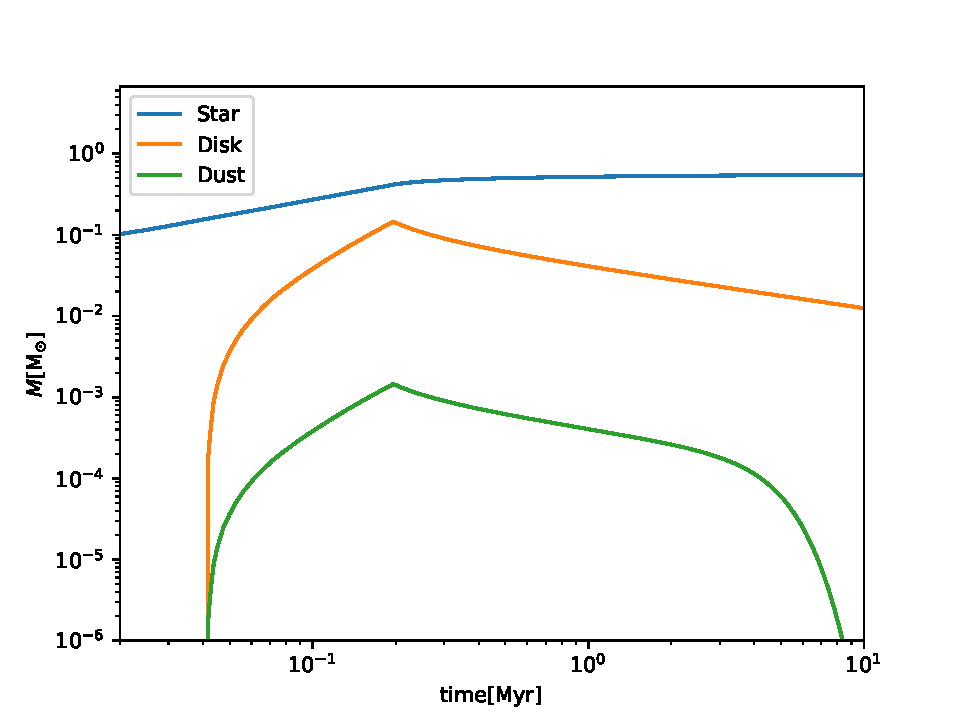
\includegraphics[width=0.7\textwidth]{../snippets/fig_snippet_infall_2_1.pdf}}
The decline of the dust compared to the gas for large times is due to the
dust radial drift.

If we have strong infall and yet low $\alpha$ turbulence, the disk tends to
become so dense, that the Toomre $Q$ value drops below 2. Physically this means
that the disk becomes gravitationally unstable, leading to spiral waves, which
redistribute angular momentum and matter. The normal viscous disk evolution
equations do not handle this properly. In Section \ref{sec-grav-instab} we
discuss a simplified method to deal with this. If we apply this at every time
step during the infall phase, we can prevent unphysically dense disks from
emerging. In other words: we mimic the mass-spreading effect of the
gravitational instability to keep $Q\ge 2$ everywhere.

The code snippet is
\code{snippet\_infall\_3.py}. In Python run it as:
\begin{codebox}
%run snippet_infall_3.py
\end{codebox}
The evolution of the surface density is shown here:\\
\centerline{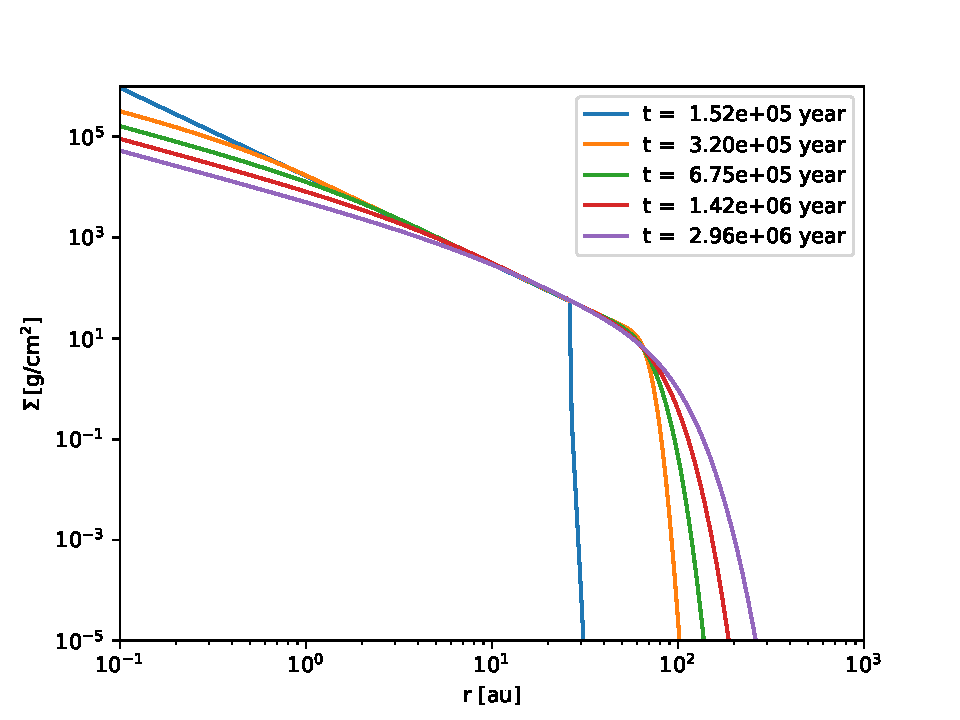
\includegraphics[width=0.7\textwidth]{../snippets/fig_snippet_infall_3_2.pdf}}
and the evolution of the Toomre $Q$ parameter here:\\
\centerline{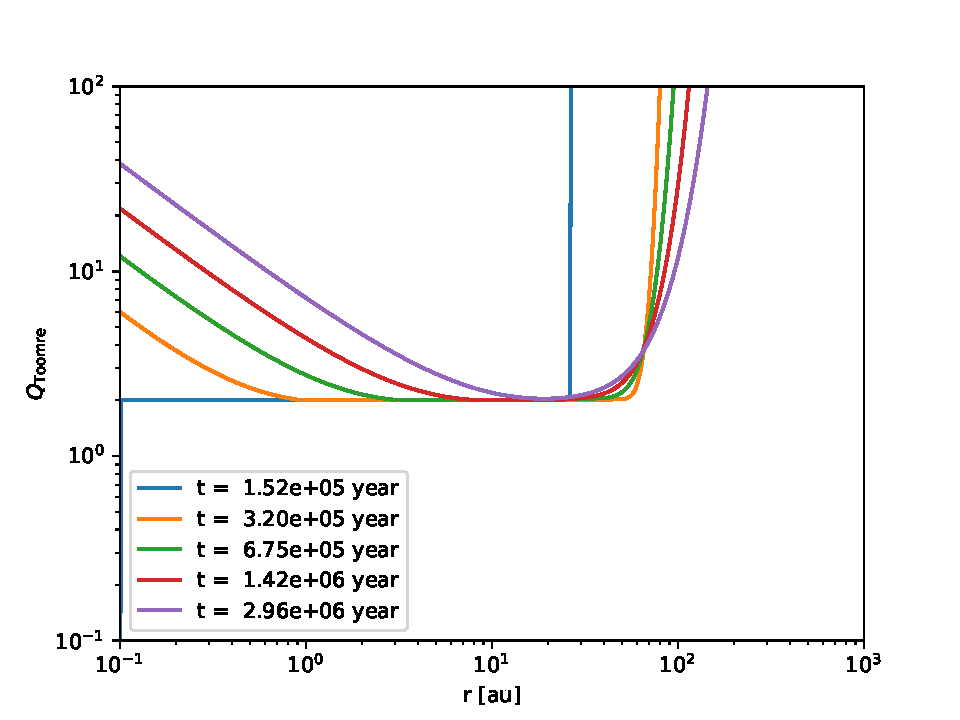
\includegraphics[width=0.7\textwidth]{../snippets/fig_snippet_infall_3_3.pdf}}
One sees that the gravitational instability treatment of
Section \ref{sec-grav-instab}, applied here, keeps the Toomre
$Q$ above 2, and the disk (marginally) stable.

Finally, code snippet \code{snippet\_infall\_4.py} demonstrates that it can save
computational time to start the model only once the centrifugal radius of the
infall reaches the inner edge of the radial grid. This is because at earlier times
there is anyway no disk yet. The initial stellar mass is then simply the infall
rate times the starting time. 

\section{Numerical stability with viscous heating and non-linear opacity model}
\label{sec-numstab-vischeat-opac-evol}
%
The time-dependent integration of the viscous disk equations in {\sf DISKLAB} is
performed using implicit integration (see Section
\ref{sec-standard-diff-eq-solver-onedee}). However, the implicit integration
method is only applied {\em partially}: It is applied to $\Sigma(r)$, keeping
everything else fixed. Under most circumstances this allows us to make
large time steps without risking numerical instability.

However, under special circumstances this approach can fail. It is known to
fail, for instance, when we include viscous heating (for the calculation of
\code{tmid}) using a mean opacity model that includes dust evaporation
``jumps''. The Bell \& Lin opacity model (Section \ref{sec-mean-opac-bellin})
includes this, for instance. For increasing temperature the opacity makes
sudden jumps downward. 

An example of how this fails is given in the following snippet:
\code{snippet\_viscevol\_instability\_1.py}. In Python run it as:
\begin{codebox}
%run snippet_viscevol_instability_1.py
\end{codebox}
The evolution of the surface density is shown
here:\\ \centerline{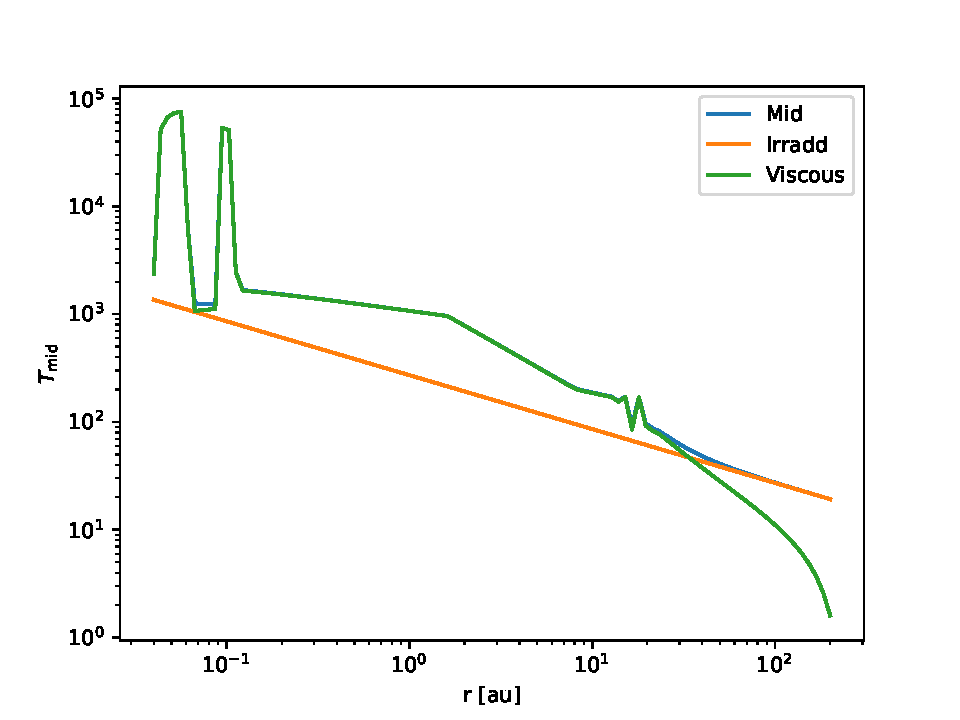
\includegraphics[width=0.7\textwidth]{../snippets/fig_snippet_viscevol_instability_1_1.pdf}}
One can clearly see that the solution is wrong: it contains dramatic wiggles.
In fact, at each time step, the peaks flip back and forth. In fact, also the
surface density $\Sigma$ flips back and forth between two limits.  The product
of $\Sigma$ and $T_{\mathrm{mid}}$, however, stays well-behaved, because $\dot
M\propto \Sigma\,T_{\mathrm{mid}}$, and the implicit viscous disk evolution
algorithm tries to keep the accretion well-behaved.

The solution to this flip-flop instability is to vary $\Sigma \propto
1/T_{\mathrm{mid}}$ while solving for $T_{\mathrm{mid}}$. This can be done by
setting \code{fixmdot=True} in the call to \code{compute\_disktmid()}.
The snippet is: \code{snippet\_viscevol\_instability\_2.py}. In Python run it as:
\begin{codebox}
%run snippet_viscevol_instability_2.py
\end{codebox}
The evolution of the surface density is shown
here:\\ \centerline{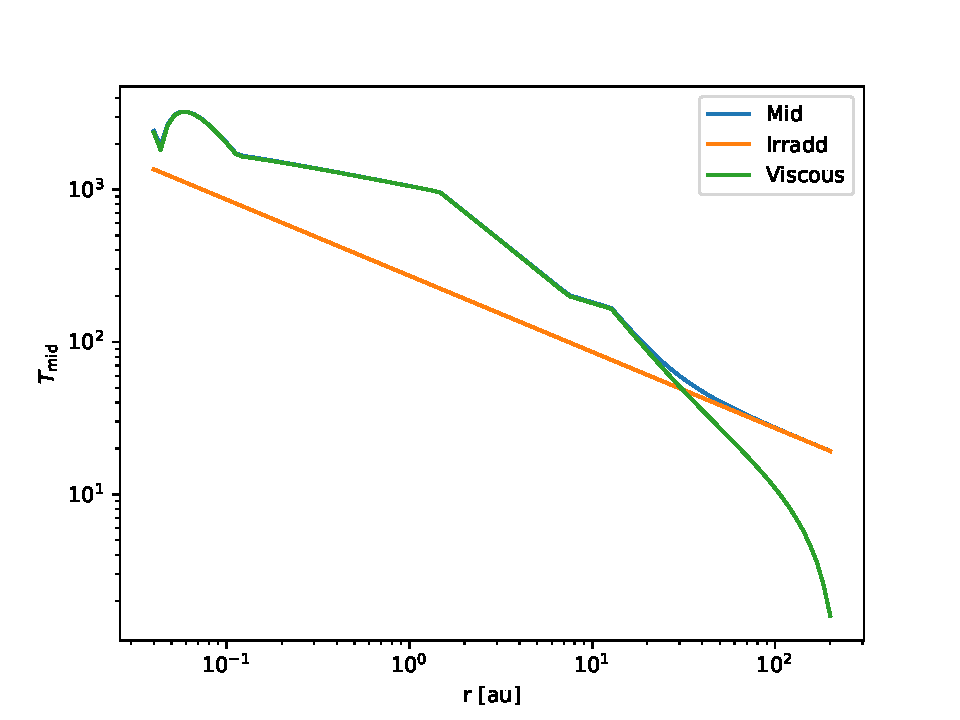
\includegraphics[width=0.7\textwidth]{../snippets/fig_snippet_viscevol_instability_2_1.pdf}}
As one can see: now everything remains well-behaved.



\section{For convenience: the {\tt DiskRadialModel.anim()} method}\label{sec-disk-standard-anim}
Sometimes it is nice to see how the disk (or some quantity of the disk)
evolves time-dependently, in an animation. The \code{DiskRadialModel.anim()}
method provides a simple way to do this.

Here is an example snippet: \code{snippet\_anim\_diskmodel\_1.py}. In Python run
it as:
\begin{codebox}
%run snippet_anim_diskmodel_1.py
\end{codebox}
Here is the listing: \lstinputlisting{../snippets/snippet_anim_diskmodel_1.py}
This should show a simple viscously spreading disk. The time snapshots are
chosen linear in time in this example.

But you can also choose a logarithmic time spacing. And you can animate any other
quantity, for instance the dust surface density (see Chapter
\ref{chap-adding-dust-component}). As a preview of this, you can enjoy the
following animation of dust drift in an evolving disk with two planetary gaps:
\code{snippet\_anim\_diskmodel\_2.py}. In Python run it as:
\begin{codebox}
%run snippet_anim_diskmodel_2.py
\end{codebox}

\section{For convenience: the {\tt viewarr.py} tool}\label{sec-viewarr}
Another way to animate the time-evolution of a model is to use the
\code{viewarr.py} tool, included in {\sf DISKLAB}. This tool makes use of the
\code{interactive\_plot.py} tool, also available in {\sf DISKLAB}.

\code{viewarr.py} is a general-purpose tool to plot 1-D cuts from an
$n$-dimensional array. By storing the intermediate time snapshots into
a 2-D array, you can view the time-evolution using a slider. 

Here is an example snippet: \code{snippet\_anim\_diskmodel\_3.py}. In Python run
it as:
\begin{codebox}
%run snippet_anim_diskmodel_3.py
\end{codebox}

\centerline{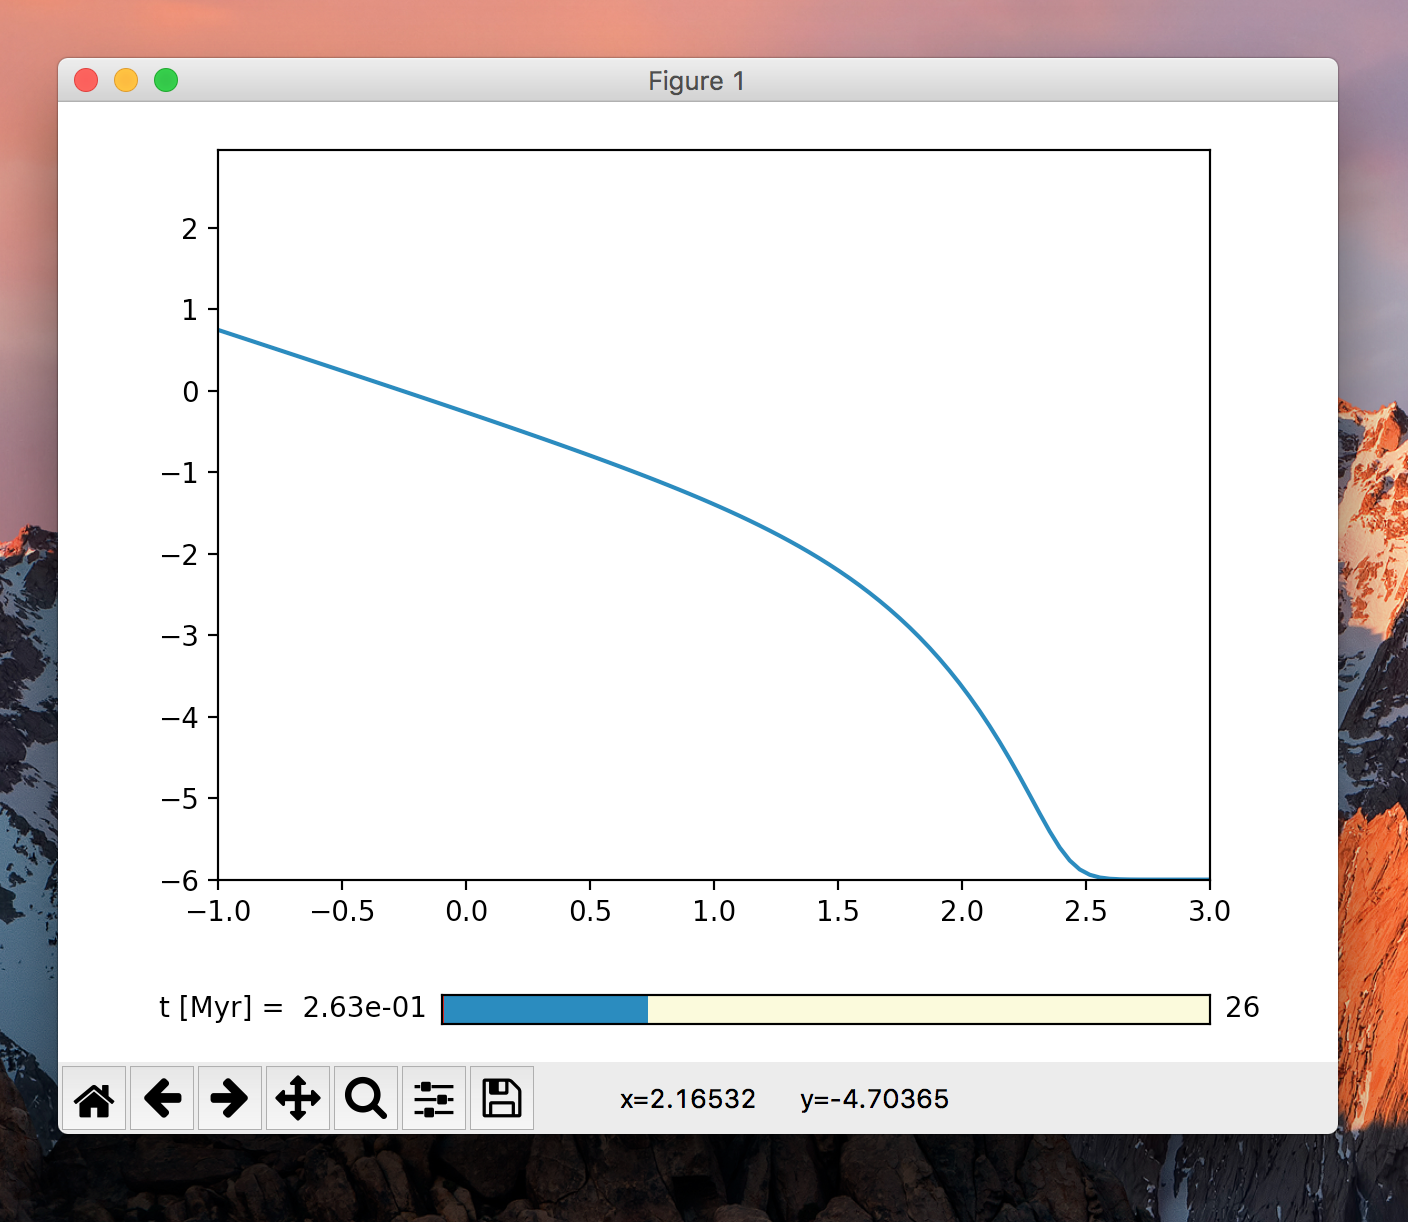
\includegraphics[width=0.7\textwidth]{viewarr_example_1.png}}

\chapter{Adding dust components to the 1-D radial disk model}
\label{chap-adding-dust-component}
\label{chap-dust-drift-mixing}
An essential feature of {\sf DISKLAB} is to include the dynamics of the dust
particles. One can include any number of different kinds of dust particles,
where each kind is a disk component, represented by an object of the class
\code{DiskRadialComponent}.

A disk component can be regarded as a gas or dust species that is part of the
disk model. Mostly we will be concerned with {\em dust} components, which can
have a different velocity and mixing characteristics from the main gas surface
density of the disk (dust drift, for example). But a disk component can also be
a {\em gas} component, for instance the vapor of sublimated ice grains. Both
dust components and gas components are described as a {\em disk} component,
and are described by objects of the class \code{DiskRadialComponent}.

For the remainder of this chapter, we will assume that the disk components
we add are, in fact, dust components.

\section{The {\tt DiskRadialComponent} class}
\label{sec-diskcomponent-class}
\label{sec-add-dust}
A dust component is added to the disk model with the \code{add\_dust()}
method. This will create a dust object from the \code{DiskRadialComponent} class, and
it will add this to a list with the name \code{dust}:
\begin{codebox}
from disklab.diskradial import *
from disklab.natconst import *
d = DiskRadialModel(mdisk=0.01*MS)
d.add_dust(agrain=1e-4,xigrain=3.6,dtg=0.1)
d.dust
Out[]: [<disklab.diskradial.DiskRadialComponent at 0x10c02f690>]
\end{codebox}
The \code{DiskRadialComponent} class is a class like \code{DiskRadialModel} but containing
not the information about the gas, but instead information about the dust (or
another type of disk component such as a chemical species).

Note that d.dust is a {\em list} of dust components. We can add several dust
components:
\begin{codebox}
from disklab.diskradial import *
from disklab.natconst import *
d = DiskRadialModel(mdisk=0.01*MS)
d.add_dust(agrain=1e-4,xigrain=3.6,dtg=0.1)
d.add_dust(agrain=1e-3,xigrain=3.6,dtg=0.1)
d.add_dust(agrain=1e-2,xigrain=3.6,dtg=0.1)
d.dust
Out[]:
[<disklab.diskradial.DiskRadialComponent at 0x10a82eb90>,
 <disklab.diskradial.DiskRadialComponent at 0x1134d67d0>,
 <disklab.diskradial.DiskRadialComponent at 0x1134d6510>]
\end{codebox}
And like any Python list, we can remove items from the list, e.g.
\begin{codebox}
d.dust.pop()
Out[]: <disklab.diskradial.DiskRadialComponent at 0x1134d6510>
d.dust
Out[]:
[<disklab.diskradial.DiskRadialComponent at 0x10a82eb90>,
 <disklab.diskradial.DiskRadialComponent at 0x1134d67d0>]
d.dust.pop(0)
Out[]: <disklab.diskradial.DiskRadialComponent at 0x10a82eb90>
\end{codebox}

The \code{add\_dust()} method is just a shorthand for the following set of
commands:
\begin{codebox}
dust = DiskRadialComponent(d,agrain=1e-4,xigrain=3.6,sigma=d.sigma*0.1)
d.dust.append(dust)
\end{codebox}
What happens here is that we first create an instance of the class
\code{DiskRadialComponent} and call it \code{dust}. As you can see, the first
argument is \code{d} (the disk model): any disk component must know
about its `parent', which is the disk model. This is stored in
\code{dust.diskradialmodel}. But the disk component does not necessarily
know about all its dust components. Only if you append \code{dust} to
the list \code{d.dust} will the disk model \code{d} `know' about this
dust component.

Note that each dust component is just a single dust component, i.e.~a single
grain size or single Stokes number. If you want to include a {\em grain size
  distribution}, then you simply have to add, say, 10 dust components of
increasing sizes, which together represent a 10-point sampling of the size
distribution (see Section \ref{sec-multi-dust-spec}). For now we will focus on a
single species.

For each single dust component it holds that at any given radius the dust grains
have only one size $a$ in units of centimeter (given as \code{agrain}) with
material density $\xi$ in units of gram/cm$^3$ (given as \code{xigrain}).  The
grain mass $m$ is then computes as \code{mgrain} assuming a homogeneous sphere:
\begin{equation}
m=\frac{4\pi}{3}\xi a^3
\end{equation}
There is, however, an exception to this: if you specify the {\em Stokes number}
instead of the grain size, then the grain size will vary with $r$ (see below).

The computation of the {\em properties} of the dust grains are handled by a
separate class: the \code{GrainModel} class (see Chapter
\ref{chap-grain-model}). This class contains all the methods for computing
various properties of the dust and how the grains interact with the gas.
However, the surface density of the dust \code{sigma} is an attribute of the
\code{DiskRadialComponent} class (Section \ref{sec-diskcomponent-class}), not of the
\code{GrainModel} class (Chapter \ref{chap-grain-model}).  The
\code{GrainModel} class is therefore meant only for
computing dust grain properties, and at any given time contains only one single grain
with one set of properties. In other words: The \code{GrainModel} class is
meant only for properies of an {\em individual} dust grain, while the
\code{DiskRadialComponent} class describes the {\em spatial and temporal distribution}
of the dust.

When adding a dust component with the \code{add\_dust()} method, one can {\em
  either} specify the Stokes number (and the grain size will then be calculated
at each radius) {\em or} one specifies the grain size (and the Stokes number is
then calculated at each radius). One can also specify the material density $\xi$
and the dust-to-gas ratio.

Example:
\begin{codebox}
from disklab.diskradial import *
from disklab.natconst import *
d = DiskRadialModel(mdisk=0.01*MS)
d.add_dust(agrain=1e-4,xigrain=3.6,dtg=0.1)
\end{codebox}
This adds a dust component to the disk consisting of $a=1\mu m$ radius
grains with a material density of $\xi=3.6\,\mathrm{g/cm^3}$. The dust is added
at a dust-to-gas ratio of 0.1. The Stokes number at each radius is given by
\code{d.St}. One can also specify \code{St}:
\begin{codebox}
from disklab.diskradial import *
from disklab.natconst import *
d = DiskRadialModel(mdisk=0.01*MS)
d.add_dust(St=1e-2,xigrain=3.6,dtg=0.1)
\end{codebox}
You can inspect the results:
\begin{codebox}
d.dust[0].agrain   # Grain radius in cm
d.dust[0].mgrain   # Grain mass in gram
d.dust[0].tstop    # Stopping time in seconds (at the midplane of the disk)
d.dust[0].St       # Stokes number (at the midplane of the disk)
\end{codebox}
{\em Note:} The \code{[0]} means: the first dust component. In the above example
we added just one component, hence only \code{[0]}. If you add another dust
component, you can also inspect \code{d.dust[1]}.

\section{Frictional stopping time and the Stokes number}
%
The dynamics of dust grains in a protoplanetary disk is entirely
goverened by the {\em stopping time} of the grains.
In \code{DiskRadialModel} the stopping time is automatically computed when the
\code{add\_dust()} method is called. It is, for each disk component
\code{dc}, stored in \code{dc.tstop}.

But if the disk midplane temperature
\code{d.tmid} or the disk gas surface density \code{d.sigma} change, one
has to recompute the stopping time in order to obtain the correct
drift and mixing behavior. This can be done with
\begin{codebox}
for dust in d.dust:
    dust.compute_stokes_from_agrain()
\end{codebox}
The method \code{compute\_stokes\_from\_agrain()}, in fact, uses the
methods of the \code{GrainModel} class to compute the stopping time.
For more details on the {\em stopping time} and the {\em Stokes number},
and how they are computed, please see Section \ref{sec-grain-compute-tstop}.

Given the Stokes number $\mathrm{St}$, the dynamical behavior of the dust particle in
the disk can be calculated. In \code{DiskRadialModel} we always compute $\mathrm{St}$
for the radial drift and mixing from the {\em midplane} gas density and temperature.

In principle the Stokes number is automatically computed by \code{add\_dust()} if
\code{agrain} is specified, and vice versa. But sometimes it can happen that you
do not want to re-call \code{add\_dust()} but you want to re-compute the Stokes
number and stopping time (because, e.g., the disk temperature has changed). You
can do that with\\ \code{compute\_stokes\_from\_agrain()}. The reverse method is
\code{compute\_agrain\_from\_stokes()}.

{\bf Warning:} For large particles and high gas density, the gas drag formulae
will be in the {\em Stokes regime}. In that case, the computation of the
stopping time will depend on the relative velocity between the dust and the gas
$|v_{\mathrm{dust}}-v_{\mathrm{gas}}|$. You must then specify this relative velocity
in your call to \code{dust.compute\_stokes\_from\_agrain()}. There is a numerical
subtlety here: in \code{DiskRadialModel} and \code{DiskRadialComponent} the radial velocity
is specified at the cell interfaces, not at the cell centers. To not complicate
matters too much, we can simply use those (shifting half a cell):
\begin{codebox}
for dust in d.dust:
    dust.compute_stokes_from_agrain(dv=np.hstack((np.abs(d.vr-dust.vr),0.)))
\end{codebox}
And you may need to iterate this with the computation of the radial dust drift
velocity (see Section \ref{sec-comp-vdrift}). So indeed, for large particles
(larger than the molecular mean-free path of the gas), things become a bit
tricky. {\bf Designing a convenient automatic iteration procedure for this is on
  our to-do-list (2018.04.14).}


\section{Computation of radial dust velocity $v_{\mathrm{dust}}$}
\label{sec-comp-vdrift}
The method \code{compute\_dustvr\_at\_interfaces()} computes the dust radial
drift velocity $v_{\mathrm{dust}}$. The method first computes the radial
velocity of the gas $v_r$ (see Subsection \ref{sec-comp-mdot-vr}), which is important,
because the gas flow can drag the dust along with it. It relies on the
already-computed Stokes number of the dust (\code{self.St}, computed as
described in Section \ref{sec-add-dust}). We follow here again Birnstiel,
Dullemond \& Brauer (2010) A\&A 513, 79. Accordingly:
\begin{equation}\label{eq-radial-dust-velocity}
  v_{\mathrm{dust}} = \frac{1}{1+\mathrm{St}^2} \left(v_r +
  \mathrm{St} \frac{c_s^2}{\Omega_Kr}\frac{d\ln p}{d\ln r}\right)
\end{equation}
where $p$ is the gas pressure at the midplane $p=\rho c_s^2$, and $d\ln p/d\ln
r$ is the double-logarithmic derivative of the gas pressure, which is computed
in the method \code{compute\_omega()} (see Section
\ref{sec-compute-omega}).  Note that for $\mathrm{St}\rightarrow 0$ we obtain
$v_{\mathrm{dust}} \rightarrow v_r$, i.e.~the dust is then perfectly coupled to
the gas, moving along with it. Conversely, for $\mathrm{St}\rightarrow \infty$
we obtain $v_{\mathrm{dust}} \rightarrow 0$.

\section{Time-dependent radial dust drift and mixing}
\label{subsec-timedep-dustdriftmix}
The method \code{get\_dust\_radial\_drift\_next\_timestep()} lets the
dust radially drift and mix one time step. Also this method uses implicit
integration and is thus stable even for large time steps. But as with the
disk evolution: large time steps may lead to unreliable results.

We always use the midplane gas density, temperature and pressure to compute the
behavior of the dust. See \ref{sec-add-dust}. We follow Birnstiel, Dullemond \&
Brauer (2010) A\&A 513, 79. The radial drift/mixing equation for the dust
is:
\begin{equation}
  \frac{\partial \Sigma_d}{\partial t}
  + \frac{1}{r}\frac{\partial (r \Sigma_d v_d)}{\partial r}
  - \frac{1}{r}\frac{\partial }{\partial r}\left(r D_d \Sigma_g \frac{\partial }{\partial r}
  \left(\frac{\Sigma_d}{\Sigma_g}\right)\right) = \dot\Sigma_d
\end{equation}
where $v_d$ is the radial dust velocity given by
Eq.~(\ref{eq-radial-dust-velocity}), and the diffusion coefficient $D_d$ is
\begin{equation}
D_d = \frac{1}{\mathrm{Sc}}\,\frac{1}{1+\mathrm{St}^2}\,\nu
\end{equation}
where $\mathrm{Sc}$ is the Schmidt number of the gas defined as the ratio of
gas turbulent viscosity $\nu$ over gas turbulent diffusivity $D_g$:
\begin{equation}
\mathrm{Sc} = \frac{\nu}{D_g}
\end{equation}
The $\mathrm{St}$ is the Stokes number of the particles given by
Eq.~(\ref{eq-define-stokes-number}) and $\nu$ is the turbulent viscosity given
by Eq.~(\ref{eq-ss-alpha-visc}). If the source term $\dot\Sigma_d$ is positive,
then this means that dust is added to the disk. Typically this would simply
accompany infall of gas. One would then expect $\dot\Sigma_d/\dot\Sigma_g$ to
represent the dust-to-gas ratio of the infalling matter.

{\em IMPORTANT NOTE:} If you use this at the same time as the time-dependent
evolution of the gas surface density (see the {\small\tt
  get\_viscous\_evolution\_next\_timestep} method of \code{DiskRadialModel} described
in Subsection \ref{sec-time-dep-visc-disk}), then you have to keep in mind that
small enough time steps have to be made to keep the radial dust drift velocity
consistent with the changing gas. Also note that for a given grain size the
Stokes number changes as the disk evolves.

Example: a fixed gas disk with drifting dust. The code snippet is
\code{snippet\_dustdrift\_1.py}. In Python run it as:
\begin{codebox}
%run snippet_dustdrift_1.py
\end{codebox}
Here is the listing:
\lstinputlisting{../snippets/snippet_dustdrift_1.py}
\centerline{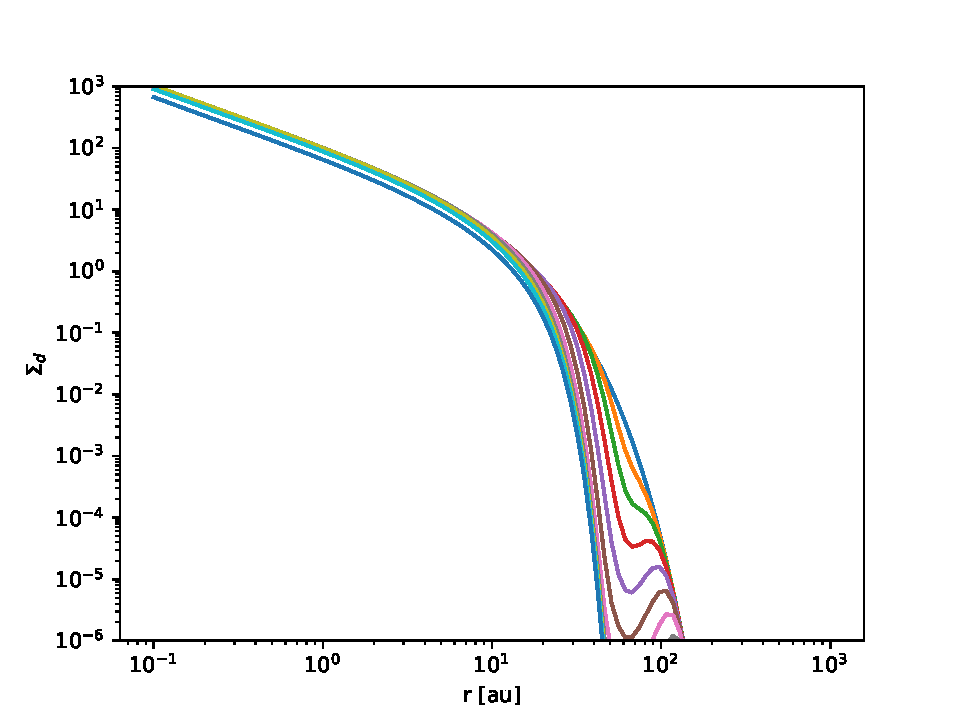
\includegraphics[width=0.7\textwidth]{../snippets/fig_snippet_dustdrift_1_1.pdf}}

Here we gave the argument \code{fixgas=True}, which means that the radial gas
velocity is not included in the dust drift: the gas is assumed to stand
still. This is useful for this example, because we do not viscously evolve the
gas disk here. If we would not include \code{fixgas=True}, then we would get an
inconsistent result: the gas is not moving, but the dust ``thinks'' that the gas
is moving. By setting \code{fixgas=True} the gas is kept fixed ($v_r=0$) (even
if \code{d.vr}$\ne 0$). The print statement gives the dust mass at each of the
time steps. One sees that the dust mass decreases. That is because radial
turbulent mixing transports dust inward where it is lost (while the gas is kept
fixed). If you uncomment the line with \code{d.Sc=1e10} you switch off the
radial mixing. You will then see no decrease of the dust mass.

Now let us do a simultaneous viscous disk evolution and dust drift/mixing
model. The code snippet is
\code{snippet\_dustdrift\_2.py}. In Python run it as:
\begin{codebox}
%run snippet_dustdrift_2.py
\end{codebox}
Here is the listing:
\lstinputlisting{../snippets/snippet_dustdrift_2.py}
\centerline{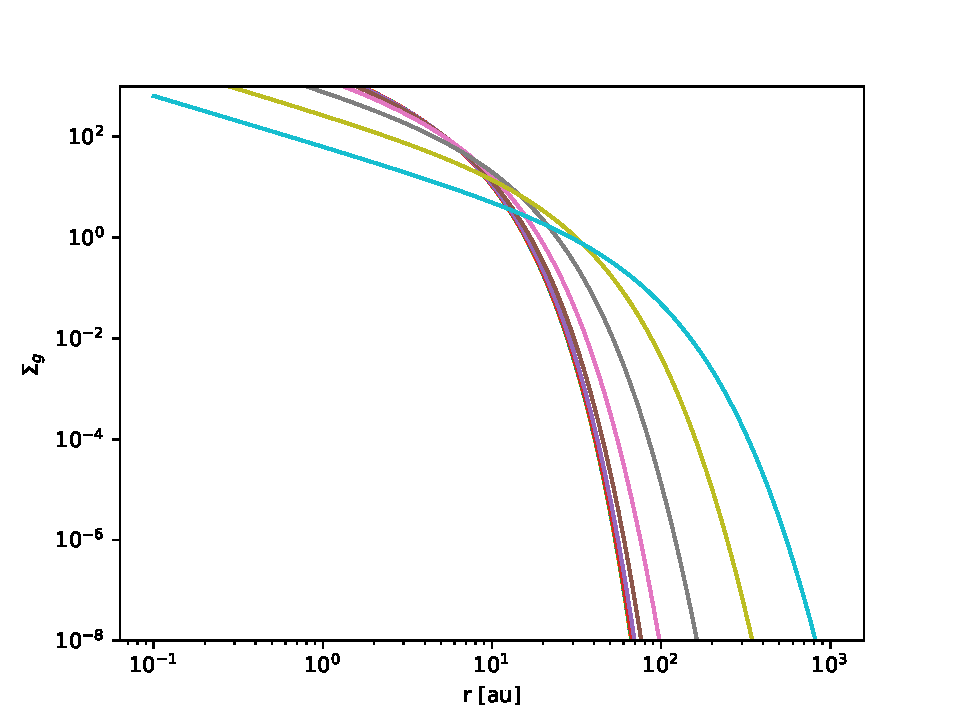
\includegraphics[width=0.5\textwidth]{../snippets/fig_snippet_dustdrift_2_1.pdf}
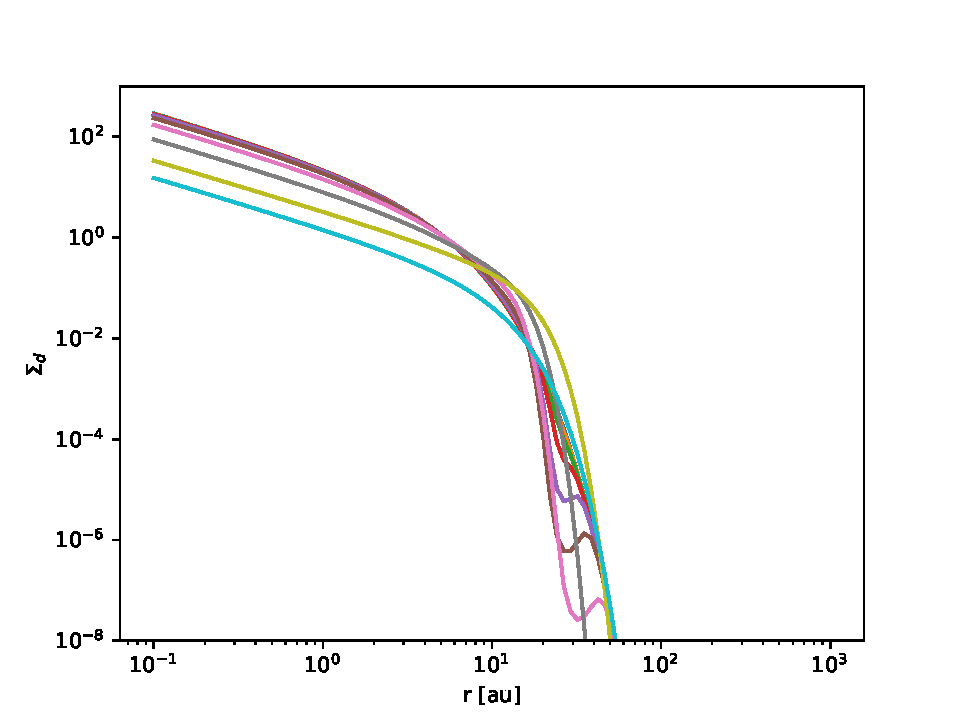
\includegraphics[width=0.5\textwidth]{../snippets/fig_snippet_dustdrift_2_2.pdf}}
Left is the gas evolution, right the dust evolution.
The commented-out command to recompute the disk midplane temperature is
here only to keep in mind that if you improve the model to include
the viscous energy dissipation (which depends on \code{d.sigma} and
\code{d.dust.sigma})
or if the irradiation flux depends on the \code{d.dust.sigma}, you would have to
recompute the midplane temperature. In this simple example this is
not the case, so it is commented-out.

The \code{DiskRadialModel} also has shortcuts for the stuff inside the time
loop. You can, for instance, replace the time loop in the above code
with:
\begin{codebox}
for itime in range(1,ntime+1):
   dt = time[itime]-time[itime-1]
   d.compute_viscous_evolution_next_timestep(dt)
   d.dust[0].compute_dust_radial_drift_next_timestep(dt)
   dlist.append(copy.deepcopy(d))
\end{codebox}
Or even shorter (by combining the viscous and dust steps):
\begin{codebox}
for itime in range(1,ntime+1):
   dt = time[itime]-time[itime-1]
   d.compute_viscous_evolution_and_dust_drift_next_timestep(dt)
   dlist.append(copy.deepcopy(d))
\end{codebox}

Here follows an example where the total dust and gas mass as a function of time
is shown in a plot, and where the dust surface density is animated
as it evolves with time.

The code snippet is
\code{snippet\_dustdrift\_3.py}. In Python run it as:
\begin{codebox}
%run snippet_dustdrift_3.py
\end{codebox}

In the animation you can see in pseudo-real-time how the dust drifts and gets
stuck in a pressure bump (the pressure bump is here ``installed'' by hand in an
ad-hoc way). The total dust mass declines but levels off at some non-zero
value. This is the effect of the dust trapping in the pressure bump. Note that
the trapping is so efficient that at the end of the simulation the dust-to-gas
ratio at the disk midplane is much larger than unity. In a real situation
this very likely would lead to the onset of the streaming instability.

\centerline{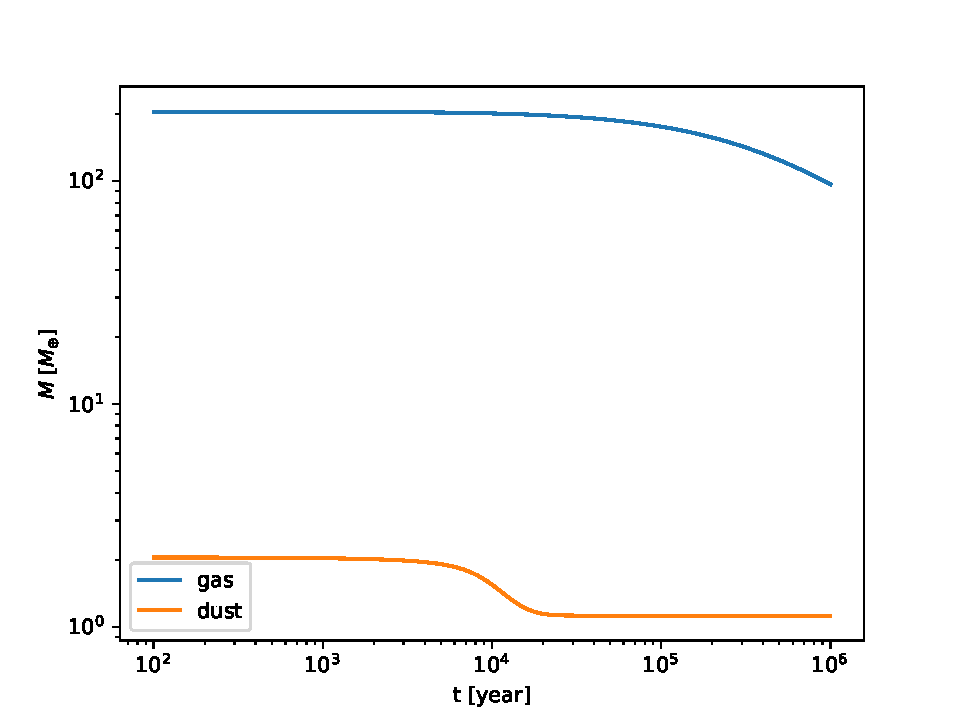
\includegraphics[width=0.5\textwidth]{../snippets/fig_snippet_dustdrift_3_1.pdf}
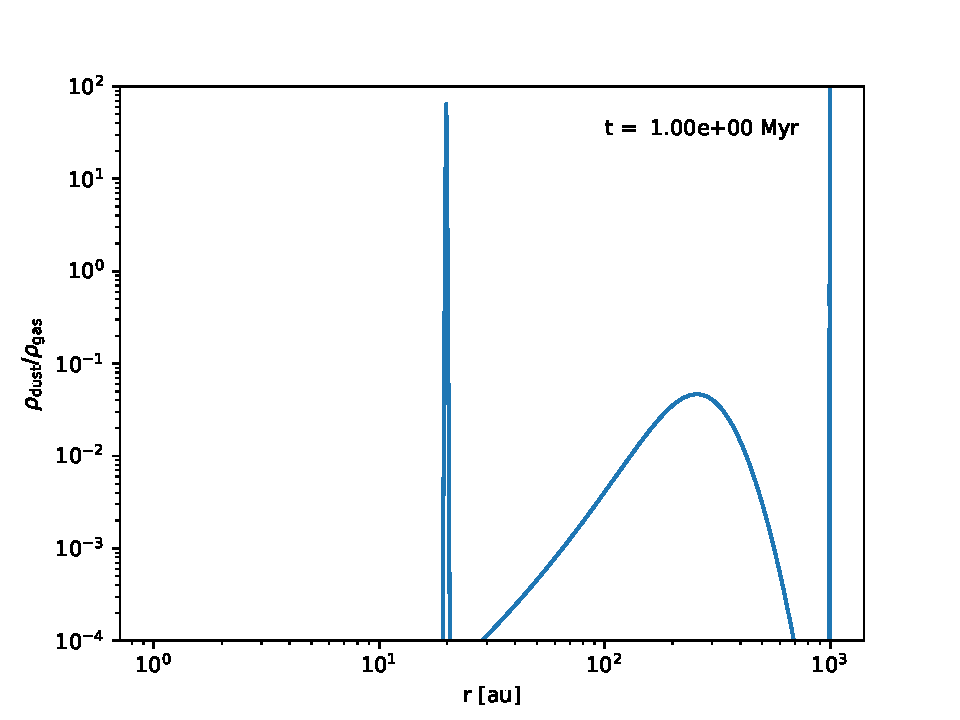
\includegraphics[width=0.5\textwidth]{../snippets/fig_snippet_dustdrift_3_2.pdf}}


\section{Steady-state radial dust drift and mixing solution}
\label{sec-dust-driftmix-steady}
Radial drift of dust is often rather rapid. We may therefore assume that
if there is dust trapping in pressure maxima, the dust is in steady state.
The main parameter is then the dust accretion rate.
The \code{get\_drift\_diffusion\_solution()} method computes this
steady-state for a given dust accretion rate.

Example of a disk with a bump. The code snippet is
\code{snippet\_dustdrift\_stationary\_1.py}. In Python run it as:
\begin{codebox}
%run snippet_dustdrift_stationary_1.py
\end{codebox}
Here is the listing:
\lstinputlisting{../snippets/snippet_dustdrift_stationary_1.py}
\centerline{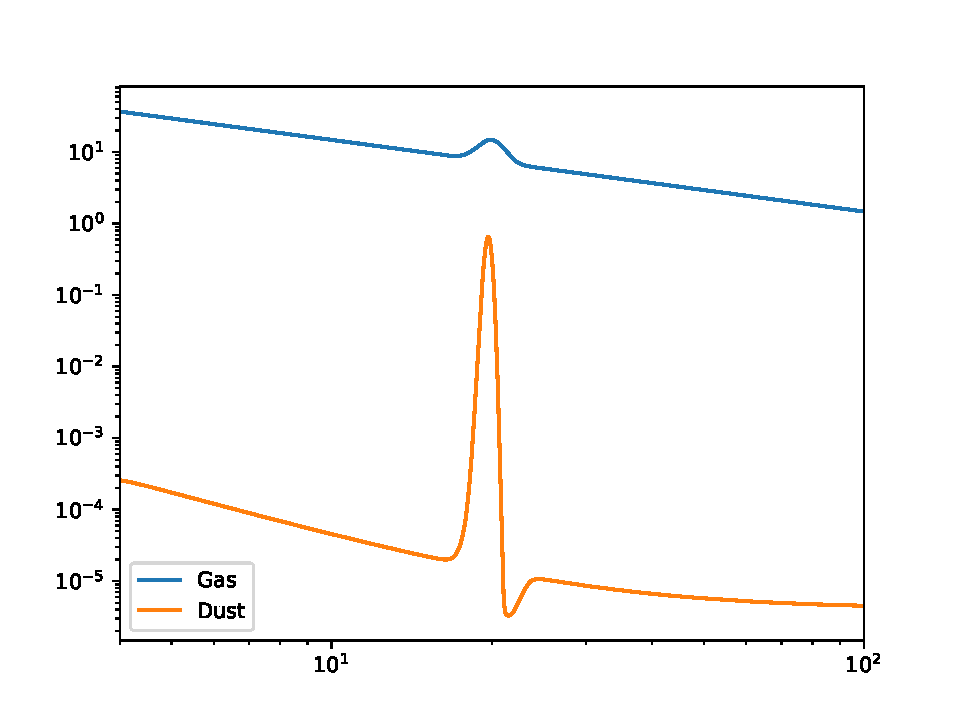
\includegraphics[width=0.7\textwidth]{../snippets/fig_snippet_dustdrift_stationary_1_1.pdf}}
Note how sensitive the result is to the viscous alpha parameter. If you plot it with
only two times weaker alpha you will find a dramatically stronger peak. This is logical
because the dust can only escape the dust trap if there is sufficiently strong mixing.
Since the dust accretion rate is fixed, the peak will then change for changing turbulence.
Note also the dip before the bump: this is because the dust will get accelerated as it
enters the dust trap.


\section{Testing dust trapping against an analytic solution}
\label{sec-dust-trap-test}
%
For very idealized situations one can compute an analytic steady-state solution
for the dust trapping scenario. We consider a narrow gas ring around the star at
radius $r_0$ with a midplane pressure given by
\begin{equation}\label{eq-gaussian-pressure-bump}
p(r) = p_0 \exp\left(-\frac{(r-r_0)^2}{2\sigma^2}\right)
\end{equation}
where $\sigma\ll r_0$ is the parameter setting the width of this gaussian ring.
One can derive that the steady state dust distribution is then:
\begin{equation}\label{eq-analytic-sol-radial-trapping}
\Sigma_{\mathrm{d}}(r) = \Sigma_{\mathrm{d0}} \exp\left(-\frac{(r-r_0)^2}{2\sigma_{\mathrm{d}}^2}\right)
\end{equation}
with
\begin{equation}
  \sigma_{\mathrm{d}} = \sigma \sqrt{\frac{\Omega_KD_{\mathrm{d}}(\mathrm{St}+\mathrm{St}^{-1})}{c_s^2}}
  = \sigma\sqrt{\frac{\alpha_{\mathrm{turb}}}{\mathrm{Sc}\,\mathrm{St}}}
\end{equation}
Note that this is only valid as long as $\alpha_{\mathrm{turb}}\ll \mathrm{Sc}\,\mathrm{St}$.

A more general solution, which is also valid for $\alpha_{\mathrm{turb}}\gtrsim
\mathrm{Sc}\,\mathrm{St}$, can be found if we specify $\mathrm{St}$ at the
peak of the bump, but allow it to rise as the gas density $\rho$ drops,
when we move away from $r_0$. The solution is then the radial version of
the solution by Fromang \& Nelson (2009) A\&A 496, 597 (their Eq.~19):
\begin{equation}\label{eq-analytic-sol-radial-trapping-better}
  \Sigma_{\mathrm{d}}(r) = \Sigma_{\mathrm{d0}} \exp\Bigg[
    -\frac{\mathrm{Sc}\,\mathrm{St}_0}{\alpha_{\mathrm{turb}}}
     \left(\exp\left(\frac{\Delta r^2}{2\sigma^2}\right)-1\right)
    -\frac{\Delta r^2}{2\sigma^2}\Bigg]
\end{equation}
where we defined $\Delta r$ as
\begin{equation}
\Delta r \equiv (r-r_0)
\end{equation}
and $\mathrm{St}_0$ is the value of the Stokes number at the peak of the
pressure bump.  

A test of the code against this analytic solution is
given in snippet \code{snippet\_dustdrift\_traptest\_1.py}.


\section{Some notes on multiple dust species or sizes}
\label{sec-multi-dust-spec}
%
\subsection{How dust species/sizes are associated to a disk model}
As shown above, it is very easy to include multiple dust species in the disk
model. Simply apply \code{add\_dust()} multiple times, and each time you do
this, a new dust component is created and added to the list \code{dust}
(i.e.\ to \code{d.dust}, if \code{d} is an object of class \code{DiskRadialModel}).
To remind you, here is how you can create three independent dust species:
\begin{codebox}
from disklab.diskradial import *
from disklab.natconst import *
d = DiskRadialModel(mdisk=0.01*MS)
d.add_dust(agrain=1e-4,xigrain=3.6,dtg=0.1)   # The first dust component
d.add_dust(agrain=1e-3,xigrain=3.6,dtg=0.02)  # The second dust component
d.add_dust(agrain=1e-2,xigrain=3.6,dtg=0.001) # The third dust component
\end{codebox}
You can, alternatively, also create a new component yourself and add them
to the list by hand:
\begin{codebox}
from disklab.diskradial import *
from disklab.natconst import *
d = DiskRadialModel(mdisk=0.01*MS)
dust1 = DiskRadialComponent(d,agrain=1e-4,xigrain=3.6,sigma=self.sigma*0.1)
dust2 = DiskRadialComponent(d,agrain=1e-3,xigrain=3.6,sigma=self.sigma*0.02)
dust3 = DiskRadialComponent(d,agrain=1e-2,xigrain=3.6,sigma=self.sigma*0.001)
d.dust.append(dust1)
d.dust.append(dust2)
d.dust.append(dust3)
\end{codebox}
This has exactly the same effect.

In fact, strictly speaking, you do not even need to append these components to
\code{d.dust}. If you do not append them to this list, then these components can
still be 'live', but the disk model \code{d} will not 'know' about their
existence. That is no problem, as long as you do not use methods of
\code{DiskRadialModel} that require knowledge of the dust components (such as when
using the one-zone radiative transfer method, see Section
\ref{sec-simple-radtrans}). So the following code would work fine:
\begin{codebox}
from disklab.diskradial import *
from disklab.natconst import *
ntime  = 10
d = DiskRadialModel(mdisk=0.01*MS)
dust1 = DiskRadialComponent(d,agrain=1e-4,xigrain=3.6,sigma=self.sigma*0.1)
dust2 = DiskRadialComponent(d,agrain=1e-3,xigrain=3.6,sigma=self.sigma*0.02)
dust3 = DiskRadialComponent(d,agrain=1e-2,xigrain=3.6,sigma=self.sigma*0.001)
for itime in range(1,ntime+1):
   dust1.sigma=d.dust1.get_dust_radial_drift_next_timestep(time[itime]-time[itime-1],fixgas=True)
   dust2.sigma=d.dust2.get_dust_radial_drift_next_timestep(time[itime]-time[itime-1],fixgas=True)
   dust3.sigma=d.dust3.get_dust_radial_drift_next_timestep(time[itime]-time[itime-1],fixgas=True)
\end{codebox}
Here the dust components are modelled, even though they have not been appended
to the disk model \code{d}.

Nevertheless it is often better to append them to the disk model, because methods such
as \code{d.compute\_viscous\_evolution\_and\_dust\_drift\_next\_timestep()} or
\code{d.compute\_onezone\_intensity()} will take their dust information only from
the list \code{d.dust}.

By the way, an object of the \code{DiskRadialComponent} class always ``knows'' its
master: it knows which object of the \code{DiskRadialModel} class it belongs to. You
can see this from the following example:
\begin{codebox}
from disklab.diskradial import *
from disklab.natconst import *
d = DiskRadialModel(mdisk=0.01*MS,mstar=2*MS)
dusttogasratio = 0.02
myowndust = DiskRadialComponent(d,sigma=dusttogasratio*d.sigma,agrain=1e-2)
print('Star mass is: {} Msun'.format(myowndust.diskradialmodel.mstar/MS))
\end{codebox}
But conversely: an object of the \code{DiskRadialModel} class does not necessarily
know all the dust components it owns, unless they are all added to the list
\code{d.dust}. This is automatically the case if they were generated using
\code{d.add\_dust()}.

\subsection{Dust components: from Python list to NumPy array, and back}
\label{sec-convert-dust-list-array}
Sometimes it can be unfavorable that the dust components are in a Python list
rather than a NumPy array. This is, for instance, the case when you have
multiple grain sizes, where each grain size is a dust component. At a given
radius $r$ you may want to analyze the grain size distribution, which is a
function of grain size $a$. We thus want to have a function $\Sigma_\mathrm{d}(a)$,
or in other words: an array \code{sigma[ia]}, where \code{ia} is the index for
grain size. But because the dust components are added to the disk model as a
Python list (instead of a NumPy array), this index \code{ia} is thus a
list index, not an array index. That precludes many of the powerful NumPy
methods for array manipulation.

To ameliorate this, you can simply create your own NumPy array out of the
list:
\begin{codebox}
from disklab.diskradial import *
from disklab.natconst import *
d = DiskRadialModel(mdisk=0.01*MS)
agrains      = np.array([1e-4,1e-3,1e-2,1e-1,1.0])
abundances   = 1e-3*(agrains/1e-1)**(1./6.)
for i in range(len(agrains)):
    d.add_dust(agrain=agrains[i],dtg=abundances[i])
nr = len(d.r)
na = len(agrains)
sigmadust = np.zeros((nr,na))
for ia in range(na):
    sigmadust[:,ia] = d.dust[ia].sigma[:]
\end{codebox}
For convenience {\sf DISKLAB} offers a method for that: You can replace the last
5 lines with:
\begin{codebox}
sigmadust = d.dust[0].join_multi_array(d.dust)
\end{codebox}
And once you manipulated \code{sigmadust} and want to put the results back
into the \code{d.dust} list, you can use:
\begin{codebox}
d.dust[0].return_multi_array(d.dust,sigmadust)
\end{codebox}

\subsection{A note on grain size distributions}
If we have a distribution of grain sizes in our disk, then the drift and mixing
behavior of each of these grain sizes is different. We thus need to sample the
grain size in terms of a discrete set of grain radii $a_i$ with
$i=0,\cdots,n-1$, and equivalently grain masses $m_i$. Here $n$ is the number of
sampling points in grain size.

In {\sf DISKLAB} this is handled by adding $n$ dust components to the disk
model.  Each component can drift and mix independently. Whenever you need to
study the grain size distribution at a given radius, you can use the methods
\code{join\_multi\_array()} and \code{return\_multi\_array()} described in
Section \ref{sec-convert-dust-list-array}.

The precise definition of a {\em grain size distribution} sometimes leads to
confusion, so let us define it here precisely. Suppose we want to model a
powerlaw grain size distribution:
\begin{equation}\label{eq-powerlaw-grain-size-distribution}
N(a) = N_0 (a/a_0)^{\gamma}
\end{equation}
between the sizes $a_\mathrm{min}$ and $a_\mathrm{max}$. The choice of $a_0$ is
arbitrary. For $\gamma=-3.5$ we have the usual Mathis, Rumpl \& Nordsieck (MRN)
distribution.

We have to normalize this distribution (i.e.\ choose $N_0$) such that the total
surface density of dust is $\Sigma_{\mathrm{d}}$ in units of gram per square
centimeter, because this is usually the parameter we wish to set (instead of the
more abstract $N_0$). We thus have
\begin{equation}\label{eq-graindistr-sigmatot}
\Sigma_{\mathrm{d}}=\int_{a_{\mathrm{min}}}^{a_{\mathrm{max}}}N(a)m(a)da
\end{equation}
where $m(a)$ is the grain mass
\begin{equation}
m(a) = \frac{4\pi}{3}\xi\,a^3
\end{equation}
where $\xi$ is the material density of the grain in gram per cubic centimeter.

We now want to sample this grain size distribution using $n$ grain sizes.
Since it is likely that $a_{\mathrm{max}}\gg a_{\mathrm{min}}$, it is best to
use a logarithmic spacing in $a$. Here is a recommended way to divide this
domain up in uniformly logarithmically spaced domains:
\begin{codebox}
import numpy as np
n           = 20
amin        = 1e-5    # 0.1 micron
amax        = 1e-3    # 10 micron
agraini     = amin * (amax/amin)**np.linspace(0.,1.,n+1)
agrain      = 0.5 * ( agraini[1:] + agraini[:-1] )
\end{codebox}
Here \code{agraini} are the interfaces of the `grid cells' in $a$-space, and
\code{agrain} are the cell centers. Mathematically this is often written as
\begin{equation}
a_{i-1/2} = \mathrm{agraini[i]}, \qquad a_{i} = \mathrm{agrain[i]}
\end{equation}
where $a_{i-1/2}$ are the left cell interfaces belonging to cells $i$, and $a_i$
are the cell centers. Note that \code{agrain[0]} is not identical to
\code{amin}, because \code{amin} is the left cell wall of the first cell, not
the cell center (all 'cells' here being in $a$-space, also often called 'grain
size bins'). The corresponding grain masses are:
\begin{codebox}
xi          = 3.6     # Material density of the grain in g/cm^3
mgrain      = (4.*np.pi/3.)*xi*agrain**3
\end{codebox}

A grain size distribution in {\sf DISKLAB} is simply a set of surface densities
$\Sigma_i$, one for each 'grain size bin'. How does this relate to the grain size
distribution of Eq.~(\ref{eq-powerlaw-grain-size-distribution})? To see this, we
have to integrate Eq.~(\ref{eq-powerlaw-grain-size-distribution}) over each cell:
\begin{equation}
\Sigma_{i}=\int_{a_{i-1/2}}^{a_{i+1/2}}N(a)m(a)da
\end{equation}
which is the same as Eq.~(\ref{eq-graindistr-sigmatot}), but now over a single
size bin only. For the powerlaw distribution of Eq.~(\ref{eq-powerlaw-grain-size-distribution})
we obtain
\begin{equation}
  \Sigma_{i} = \frac{4\pi}{3}\frac{N_0\xi}{(\gamma+4)a_0^\gamma}\left[a_{i+1/2}^{\gamma+4}-
    a_{i-1/2}^{\gamma+4}\right]
\end{equation}
However, if the spacing is small enough (i.e.\ $n$ is large enough), then we can
simplify this in the following way:
\begin{equation}
\Sigma_{i}=\int_{a_{i-1/2}}^{a_{i+1/2}}N(a)m(a)da=\int_{\ln a_{i-1/2}}^{\ln a_{i+1/2}}N(a)m(a)a\,d\ln a
\end{equation}
which leads to
\begin{equation}\label{eq-sigmai-from-logspace}
\Sigma_i \simeq \frac{4\pi}{3}\frac{N_0\xi}{a_0^\gamma}a_i^{\gamma+4}\,\Delta\ln a_i
\end{equation}
where
\begin{equation}
\Delta\ln a_i = \ln a_{i+1/2} - \ln a_{i-1/2}
\end{equation}
For a logarithmically equally spaced grid in $a$ we have that $\Delta\ln a_i$ is a
constant with $i$. We therefore conclude that a grain size distribution according
to Eq.~(\ref{eq-powerlaw-grain-size-distribution}) can be represented by a set of
surface densities $\Sigma_i$ such that
\begin{equation}
\Sigma_i = \Sigma_{00} \left(\frac{a_i}{a_0}\right)^{\gamma+4}
\end{equation}
In principle $\Sigma_{00}$ follows from Eq.~(\ref{eq-sigmai-from-logspace}). But given
that Eq.~(\ref{eq-sigmai-from-logspace}) is only approximate, it is better to
determine $\Sigma_{00}$ directly by the normalization:
\begin{equation}
\sum_{i=0}^{n-1} \Sigma_i = \Sigma_{\mathrm{d}}
\end{equation}
where $\Sigma_{\mathrm{d}}$ is the total dust surface density (see also
Eq.~\ref{eq-graindistr-sigmatot}).

And so we recommend the following implementation of a powerlaw size distribution:
\begin{codebox}
gamma   = -3.5    # Here the example of an MRN distribution
abun    = agrain**(gamma+4.)
abun   /= abun.sum()
\end{codebox}
where \code{abun} is the abundance of grain size $i$, normalized such that
the sum of all abundances is 1.

To summarize, here is a snippet that implements an MRN size distribution
into a disk model, and makes a plot of
\begin{equation}
\frac{d\Sigma_{\mathrm{d}}}{d\ln a} = \frac{\Sigma_i}{\Delta \ln a_i}
\end{equation}
The code snippet is
\code{snippet\_grainsize\_distribution\_1.py}. In Python run it as:
\begin{codebox}
%run snippet_grainsize_distribution_1.py
\end{codebox}
Here is the listing:
\lstinputlisting{../snippets/snippet_grainsize_distribution_1.py}
\centerline{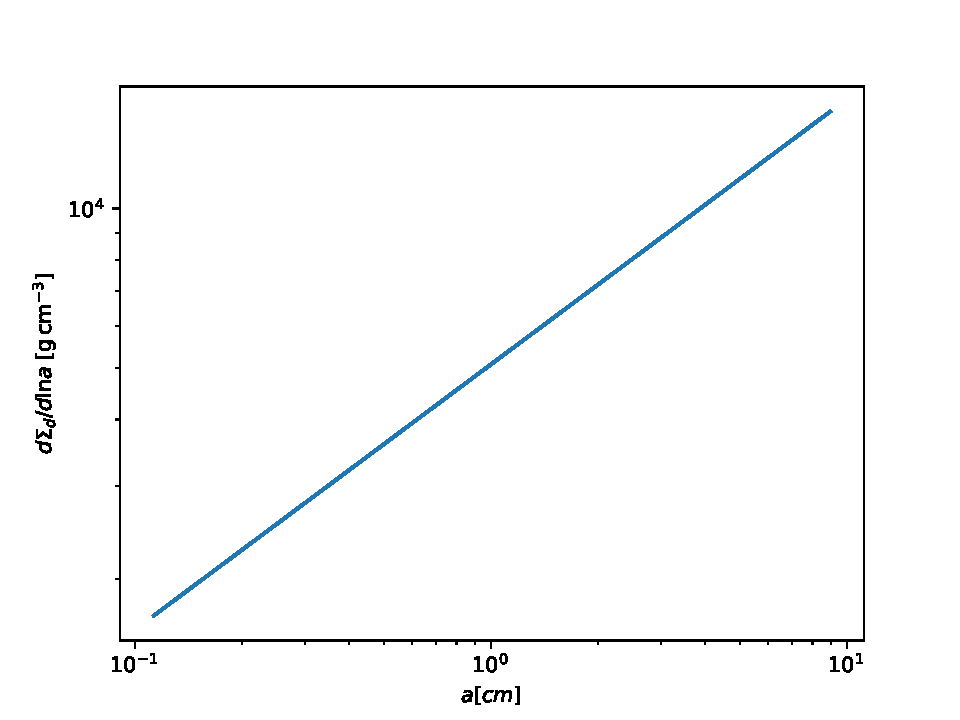
\includegraphics[width=0.7\textwidth]{../snippets/fig_snippet_grainsize_distribution_1_1.pdf}}

Note that the MRN distribution is dominated by the large grains, even though the
powerlaw is -3.5. That is a well-known property of the MRN distribution.


\chapter{Grain properties and wavelength-dependent opacities}
\label{chap-grain-model}
%
\section{The {\tt GrainModel} class}
\label{sec-grainmodel-class}
%
Dust plays a major role in protoplanetary disks. The properties of the dust
grains affect both their dynamics and their appearance (i.e.~opacities). These
grain properties are managed by the \code{GrainModel} class. A \code{GrainModel}
object contains only information about the physical properties of the grains in
question, but not about their location in the disk (which is managed by the
\code{DiskRadialComponent} class).

A \code{DiskRadialComponent} object (let's call it \code{dust}, for example) has -- or at
least should have -- a \code{GrainModel} object:
\begin{codebox}
dust.grain
\end{codebox}
Usually this \code{grain} is automatically created when you call
\code{d.add\_dust(agrain=0.1)}, for instance.

What does this object \code{grain} contain? Here is a list of its contents:
\begin{codebox}
agrain                 # Grain radius in cm (should be same as dust.agrain)
xigrain                # Material density in g/cm^3 (should be same as dust.xigrain)
mgrain                 # Grain mass in g, if computed via grain.compute_mgrain()
tstop                  # Stopping time in s, if computed using grain.compute_tstop()
species                # Name of the dust species, if given e.g. when loading
                       # opacity with e.g. grain.load_standard_opacity()
sublimationmodel       # List object specifying if/how this dust species sublimates
                       # (see main text for explaination)
opac_lammic            # (If computed or loaded) Array of wavelength in micron
                       # for opacity table.
opac_kabs              # Likewise: Array of absorption opacity kappa_abs_nu
opac_ksca              # Likewise: Array of scattering opacity kappa_scat_nu
opac_ksca_eff          # As opac_ksca, but now multiplied by (1-g),
                       # with g the forward scattering factor g=<cos(theta)>
meanopactable_tgrid            # (If computed or loaded) Temperature grid for
                               # mean opacitytable
meanopactable_kappa_planck     # Likewise: Planck mean opacity (tabulated)
meanopactable_kappa_rosseland  # Likewise: Rosseland mean opacity (tabulated)
\end{codebox}
In addition to these, the object also contains a set of methods, which we
will learn about in the coming sections.

The \code{opac\_***} attributes represent the tabulated wavelength-dependent
dust opacity for this grain. This table is not present automatically. It has to
be computed or read-in from some file (see Sections \ref{sec-reading-opacity-file}
and \ref{sec-standard-opacities}).

The \code{meanopactable\_***} attributes represent the tabulated Planck- and
Rosseland-mean opacities. Also this table is not present automatically. First
one has to load the wavelength-dependent opacity (see the \code{opac\_***}
attributes), and from these the mean opacity tables are computed (see
Section \ref{sec-grain-computing-mean-opacities}). Most methods
that read or compute the \code{opac\_***} opacity table, also automaticlly
compute the mean opacities on a standard temperature grid and store them
in the \code{meanopactable\_***} arrays.


\section{Computing the stopping time}
\label{sec-grain-compute-tstop}
%
One of the tasks of the \code{GrainModel} class is to compute the
stopping time of the grain, for a given surrounding gas density and
temperature. Here we describe how this is done.
To compute the frictional stopping time of the grain, given a gas volume density
$\rho_g$, temperature $T$ and relative velocity $\Delta v$, one uses the method
\code{compute\_tstop()} from the \code{GrainModel} class.
This subroutine follows Birnstiel, Dullemond \&
Brauer (2010) A\&A 513, 79 and Perets \& Murray-Clay (2011) ApJ 733, 56
to compute the stopping time $\tau_{\mathrm{stop}}$.
We define the thermal velocity of the gas particles $v_{\mathrm{th}}$ as
\begin{equation}
v_{\mathrm{th}} = \sqrt{\frac{8k_BT}{\pi \mu m_p}} = \sqrt{8/\pi}\,c_s
\end{equation}
with $\mu=2.3$ and $m_p$ the proton mass and $k_{\mathrm{B}}$ the Boltzmann
constant\footnote{Note that in Birnstiel, Dullemond \& Brauer (2010) the formula
  for $\bar u$ (which is their symbol for $v_{\mathrm{th}}$) uses $\bar
  u=\sqrt{\pi/8}c_s$, which is erroneous; it should be $\bar
  u=\sqrt{8/\pi}c_s$. It was correctly implemented in the code belonging to that
  paper.}. For a grain with radius $a$ and material density $\xi$ the Reynolds
number is
\begin{equation}
\mathrm{Re} = \frac{2a\Delta v}{\nu_{\mathrm{mol}}}
\end{equation}
The molecular viscosity $\nu_{\mathrm{mol}}$ is
\begin{equation}
\nu_{\mathrm{mol}} = \frac{1}{2}v_{\mathrm{th}}\lambda_{\mathrm{mfp}}
\end{equation}
where $\lambda_{\mathrm{mfp}}$ is the mean free path of the H$_2$ molecules
given by
\begin{equation}
\lambda_{\mathrm{mfp}} = \frac{1}{n_{\mathrm{gas}}\sigma_{H_{2}}}
\end{equation}
with $\sigma_{H_{2}}=2\times 10^{-15}\,\mathrm{cm}^2$ and $n$ the number density
of the gas given by
\begin{equation}
n_{\mathrm{gas}} = \frac{\rho_{\mathrm{gas}}}{\mu m_p}
\end{equation}
Note that we, for simplicity, assumed here that all particles are H$_2$, i.e.~we
ignored the He atoms.

Now the stopping time is given by Eq.~(10) of Birnstiel et al.~(2010). For small
particles ($\lambda_{\mathrm{mfp}}/a>4/9$) the Epstein regime holds:
\begin{equation}
  \tau_{\mathrm{stop}} = \frac{\xi a}{\rho_{\mathrm{gas}}v_{\mathrm{th}}}\qquad (\hbox{iff}\; \lambda_{\mathrm{mfp}}/a>4/9)
\end{equation}
For the Stokes regime (i.e.~when $\lambda_{\mathrm{mfp}}/a\le 4/9$) we refer to
Eq.~(10) of Birnstiel et al.~(2010). But for the intermediate Stokes regime
($1<\mathrm{Re}<800$) we take instead the Perets \& Murray-Clay formulae
(their Eqs. 6 and 7), which behave better. In all other regimes the two papers
are mutually consistent.

Given the stopping time, we can compute the Stokes number:
\begin{equation}\label{eq-define-stokes-number}
\mathrm{St} = \Omega_K\tau_{\mathrm{stop}}
\end{equation}
Note that in accretion disks the largest turbulent eddies have a turnover time scale
which is the same as the orbital time scale. This means that particles with $\mathrm{St}=1$
have the stopping time equal to the largest eddie time scale.

Here is an example how one can use the \code{graimmodel} class to compute
all these quantities:
\begin{codebox}
from disklab.grainmodel import *
g = GrainModel(agrain=0.1*1e-4,xigrain=2.0)  # Grain a=0.1 mum and xi=2 gram/cm^3
rhogas = 1e-10        # Gas density in g/cm^3
tgas   = 40.          # Gas temperature in K
dv     = 10.          # Velocity between dust and gas in cm/s
g.compute_tstop(rhogas,tgas,dv)
print(g.tstop)        # This gives the stopping time in seconds
\end{codebox}
which gives a number of about 3.3 seconds for this example.

The \code{DiskRadialComponent} class calls the \code{compute\_tstop()} method to compute
the stopping time and, from that, the Stokes number.

\section{Reading opacity table from file}
\label{sec-reading-opacity-file}
%
Another main task of the \code{GrainModel} class is to take care of the
wavelength-dependent dust opacities. One way to load such an opacity table
into {\sf DISKLAB} is to use the \code{grain.read\_opacity()} method. This
method simply reads an opacity table directly from a file.

There are {\em two possible opacity file formats}:
\begin{itemize}
\item The standard {\sf RADMC-3D} opacity files
  \code{dustkappa\_***.inp}, valid only for a single
  grain size. The user must be sure that the grain size
  for which this opacity file was created matches that of
  the grain model (i.e.\ matches \code{grain.agrain}). This
  is not automatically verified.
\item The {\sf DISKLAB} opacity files \code{dustkappa\_***.npz},
  which are much more flexible than the {\sf RADMC-3D} format.
  It generally contains the opacity table for a series of different
  grain sizes, so that the \code{grain.read\_opacity()} method can
  automatically find (and linearly interpolate in \code{agrain})
  the opacity wavelength-dependent opacity table.
\end{itemize}
where \code{***} can be any name of a dust compositional species
(e.g.~\code{dustkappa\_mydust.inp}).

The simplest of the two formats is the
standard {\sf RADMC-3D} opacity file format
(\code{dustkappa\_***.inp}), which is an ascii (plain
text) file. The most common form is:
\begin{codebox}
iformat                     <== This example is for iformat==3
nlam
lambda[1]        kappa_abs[1]       kappa_scat[1]      g[1]
   .                  .                  .              .
   .                  .                  .              .
lambda[nlam]    kappa_abs[nlam]   kappa_scat[nlam]    g[nlam]
\end{codebox}
That is: the first line should contain a 3, the second line the number of
wavelength points, and then a table with four columns: wavelength in micrometer,
absorption opacity in cm$^2$/gram-of-dust, scattering opacity in same units, and
the forward-scattering factor $g$ defined as the expectation value of the cosine
of the scattering angle $\theta$. See Chapter \ref{app-opacities} for
information how to create these opacity files from optical constants.
Note that the {\sf RADMC-3D} opacity file format also allows a three-column
version, in which the $g$ column is not present (first line contains 2,
i.e. \code{iformat=2}), or even a two-column version, in which also the
scattering opacity is omitted (first line contains 1, i.e. \code{iformat=1}).

The other format, i.e.\ the \code{dustkappa\_***.npz} format employs the
standard zip-compressed \code{numpy} file format. The
\code{grain.read\_opacity()} reader, when it reads an opacity file with
\code{.npz} extension, will read this file in using the standard
\code{numpy.load()} method. If you are curious as to the content of this
file, you can have a look inside:
\begin{codebox}
import numpy as np
data = np.load('dustkappa_mydust.npz')
\end{codebox}
(assuming you have created, or copied, a file of that kind, see
Chapter \ref{app-opacities}). You can then see that
the file contains a 1-D array of wavelengths in cm
called \code{lam} and another 1-D array of grain radii in cm called \code{a},
and the corresponding 2-D arrays \code{k\_abs[:,:]}, \code{k\_scat[:,:]} and
optionally \code{g[:,:]}, all three of size \code{[len(a),len(lam)]}. The
material density is given by \code{rho\_s}. When
\code{grain.read\_opacity()} reads such a file, it automatically linearly
interpolates \code{grain.agrain} in the array \code{a} of the opacity
file, and correspondingly extracts the linearly interpolated opacity
values. See Chapter \ref{app-opacities} for information how
to create these opacity files from optical constants.

Here is an example how to read and plot a {\sf DISKLAB} dust opacity file. The
standard opacity files can be found in the directory
\code{disklab/opacity/precalculated/}.

{\bf [FINISH THIS PART]}

% an opacity file. In the directory \code{opacity/}
% you will find an example opacity file called
% \code{dustkappa\_silicate.inp}. Copy this into your model directory. You can
% now use this opacity file in the following way:
% \begin{codebox}
% from disklab.diskradial import *
% from disklab.natconst import *
% d = DiskRadialModel(mdisk=0.01*MS)
% d.add_dust(agrain=0.1*1e-4,xigrain=3.6)
% d.dust[0].grain.read_opacity('dustkappa_silicate.inp')
% \end{codebox}

This will not only read the opacity table, it will also automatically calculate
the Planck- and Rosseland-mean opacities (without accounting for sublimation)
for this opacity table (see Section \ref{sec-grain-computing-mean-opacities} as
well as Chapter \ref{chap-mean-opacities}). The wavelength-dependent opacity
tables are stored in the \code{d.dust[0].grain.opac\_***} arrays.  The
precalculated mean opacities are stored in
\code{d.dust[0].grain.meanopactable\_***} (see Section
\ref{sec-grainmodel-class} and Section
\ref{sec-grain-computing-mean-opacities}).

Note that \code{dustkappa\_astrosilicate.npz} is just an example dust opacity
(the famous `astronomical silicate' model of Bruce Draine).
We discuss in Appendix \ref{app-opacities} how to create your own
opacity tables. For now we will stick with \code{dustkappa\_astrosilicate.inp}.

It is useful to inspect what the opacity looks like. So let us plot the opacity
table.

The code snippet is
\code{snippet\_plot\_dustopac\_1.py}. In Python run it as:
\begin{codebox}
%run snippet_plot_dustopac_1.py
\end{codebox}
Here is the listing:
\lstinputlisting{../snippets/snippet_plot_dustopac_1.py}
\centerline{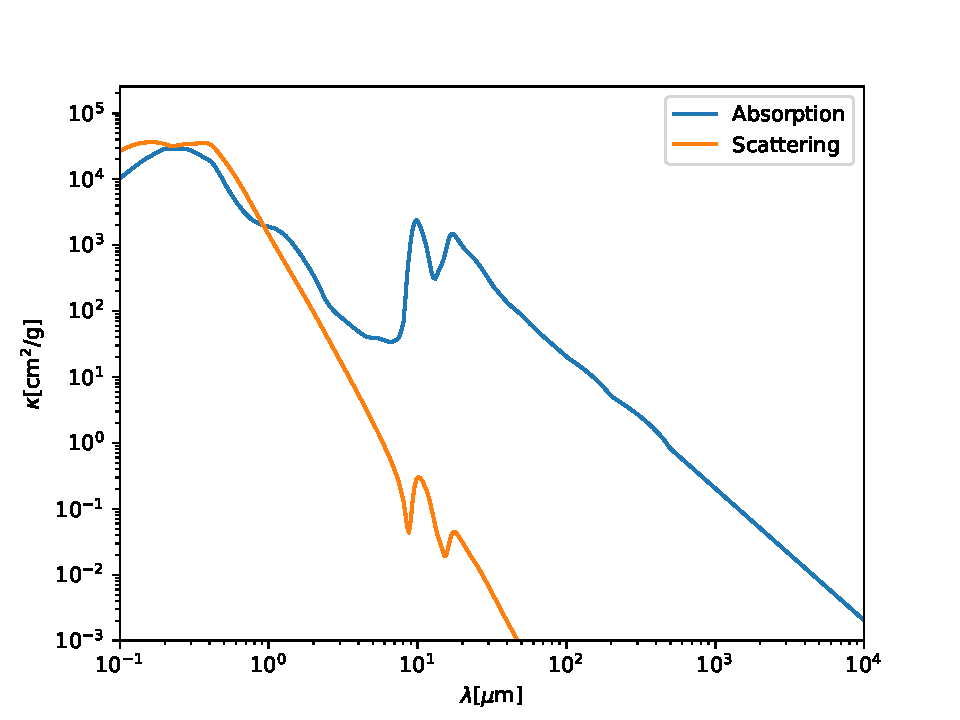
\includegraphics[width=0.7\textwidth]{../snippets/fig_snippet_plot_dustopac_1_1.pdf}}

One simple way to get the opacity at the wavelength you need is
to use numpy's \code{interp} routine:
\begin{codebox}
lammic = 1300.    # Wavelength of observation in micron
kabs   = np.interp(lammic,o.opac_lammic,o.opac_kabs)
kabs
Out: 0.12125583143387224
\end{codebox}

{\bf [MODIFY SNIPPET AND OUTPUT VALUE]}


\section{Standard precomputed opacities}
\label{sec-standard-opacities}
%
You are encouraged to create your own \code{dustkappa\_***.inp}
opacity files using a Mie code and to use these for the {\sf DISKLAB}
modeling. But very often you want to simple make some
{\em quick-n-dirty} models with some standard opacities, without
having to think hard about which opacities you really want to
compute (and how).

{\sf DISKLAB} offers a set of standard opacities for this
purpose, and a special method to read these standard opacities
in. This method is \code{load\_standard\_opacity()}.
This method is nothing fancy: it in fact uses
\code{read\_opacity()} to read in the standard opacities.
The only 'special' thing about \code{load\_standard\_opacity()} is
that you do not have to worry about {\em where} these standard
opacity files reside (FYI: they reside in the directory
\code{disklab/disklab/opacities/precalculated/}, but you do not need to know).
Note also that these precomputed standard opacities each
have their \code{.info} file containing information about
the grain radius and material density, which will automatically
be read by the method \code{load\_standard\_opacity()} as well.

Example: The code snippet is
\code{snippet\_plot\_dustopac\_3.py}. In Python run it as:
\begin{codebox}
%run snippet_plot_dustopac_3.py
\end{codebox}
Here is the listing:
\lstinputlisting{../snippets/snippet_plot_dustopac_3.py}
\centerline{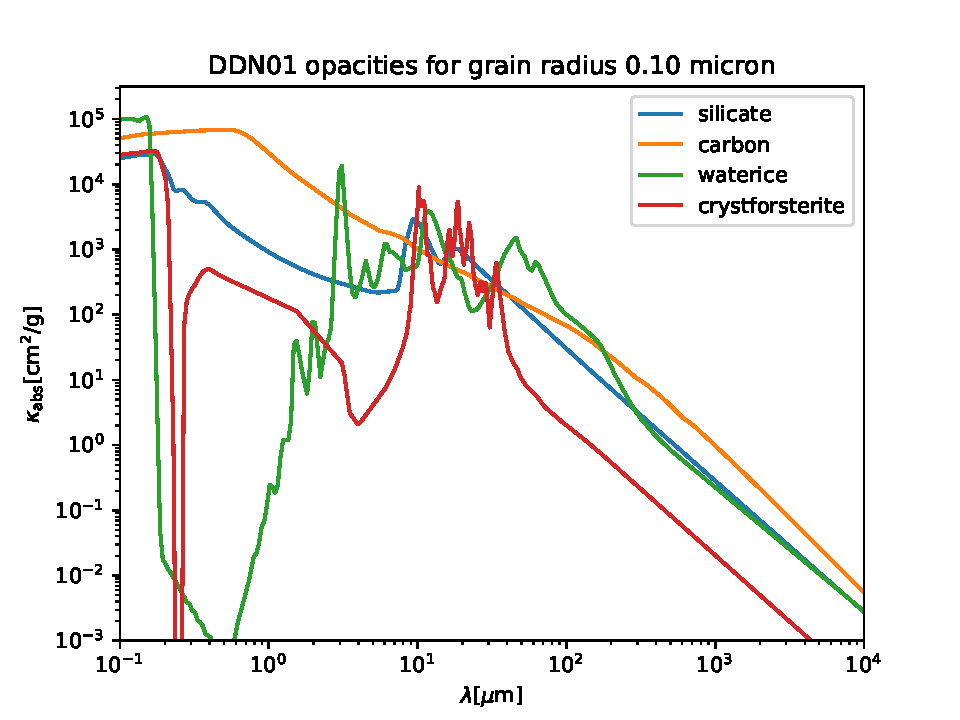
\includegraphics[width=0.7\textwidth]{../snippets/fig_snippet_plot_dustopac_3_1.pdf}}

Currently the following standard dust opacities are
built in:
\begin{center}
\begin{tabular}{ccccccc}
  Series & Name & Chem & Cryst & $\xi [\mathrm{g}/\mathrm{cm}^3]$ & $a [\mu\mathrm{m}]$ & Reference \\
  \hline
  ddn01  & silicate & MgFeSiO$_4$ & amorph & 3.6 & 0.1 & Laor \& Draine (1993) ApJ 402, 441 \\
  ddn01  & carbon   & C &  amorph & 1.8 & 0.1 & Preibisch et al.\ (1993) A\&A 279, 577 \\
  ddn01  & waterice & H$_2$O &  amorph & 1.0 & 0.1 & Warren S.G.\ (1984), Appl.Opt.\ 23, 1206 \\
  ddn01  & crystforsterite & Mg$_2$SiO$_4$ &  cryst & 3.275 & 0.1 & Servoin \& Piriou (1973) Phys.Stat.Sol.\ 55\\
\end{tabular}
\end{center}
where $\xi$ is the material density (specific weight) in gram/cm$^2$, and
$a$ is the grain radius in $\mu$m.

{\bf [REWRITE THIS SECTION]}

\section{A simple opacity model with grain-size dependence}
\label{sec-dummy-opacity-ivezic}
%
Sometimes it can be useful to use a much simpler dust opacity, in particular for
testing purposes. The method \code{grain.compute\_simple\_opacity()} computes the
simple dust opacity model of the Ivezic et al.~(1997) MNRAS 291, 121.
This simple model is:
\begin{equation}
  \kappa_\nu^{\mathrm{abs}} = \frac{\pi a^2}{m} \left\{
  \begin{matrix}
    1 & \hbox{for}\; \lambda < 2\pi a\\
    2\pi a/\lambda & \hbox{for}\; \lambda > 2\pi a
  \end{matrix}
  \right.
\end{equation}
We do not include the scattering part of the opacity of Ivezic et al., simply
because scattering is not really included in the physics of {\sf DISKLAB}.

One main advantage of this simple opacity model over the standard pre-computed
opacity tables of Section \ref{sec-standard-opacities} is that you can specify
any grain size and material density. The disadvantage is, of course, that it is
{\em highly} approximative. It does, however, obey two of the most basic
properties of dust grain opacities: that for wavelengths $\lambda\gg a$ the
absorption opacity is `by volume' (and therefore, for a given amount of dust,
does not change with grain size $a$), while for $\lambda\ll a$ the opacity is `by
surface area' (and therefore, for a given amount of dust, drops proportional to
$1/a$).

The code snippet is
\code{snippet\_plot\_dustopac\_4.py}. In Python run it as:
\begin{codebox}
%run snippet_plot_dustopac_4.py
\end{codebox}
Here is the listing:
\lstinputlisting{../snippets/snippet_plot_dustopac_4.py}
\centerline{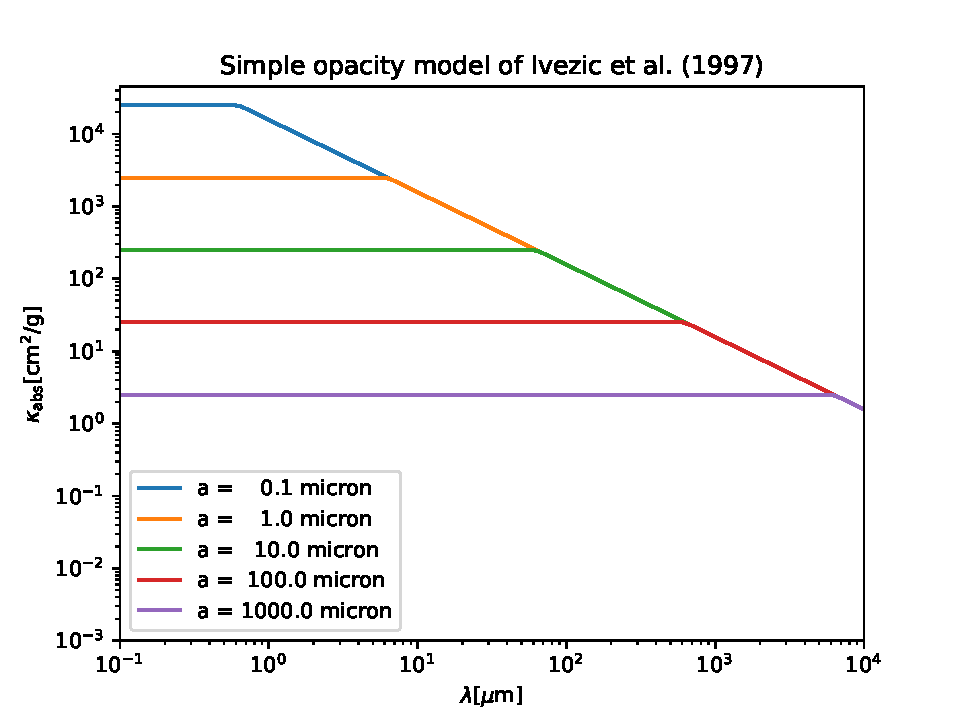
\includegraphics[width=0.7\textwidth]{../snippets/fig_snippet_plot_dustopac_4_1.pdf}}

{\bf [REWRITE THIS SECTION: IN READ STANDARD OPACITY]}

\section{Sublimation and freeze-out ('ice lines')}
\label{sec-sublimation-and-freezeout}
%
Dust grains (in particular volatile ones such as those made of ice) can only survive up to
some temperature. Above that they sublimate and disappear. Including dust opacities in
a disk model without accounting for sublimation means that the disk model will only be valid
as long as the temperatures remain below this sublimation temperature.

However, the \code{GrainModel} class provides methods to automatically reduce (or put to
zero) the abundance of a given grain species under a given set of pressure and temperature
conditions. The main method is\\ \code{GrainModel.abundance\_after\_sublimation()}. We will
discuss this method in Subsection \ref{subsec-abundance-after-sublimation}.

But first we have to tell {\sf DISKLAB} {\em how} to sublimate the dust.

\subsection{The sublimation models}
%
In the literature there are various ways and formulae to compute the temperature
of sublimation and/or the degree of sublimation for a given temperature. The
physics is complex and involves partial pressures of vapor (or vapor
components), the Hertz-Knudsen equation, and equilibrium vapor pressures
calculated from Gibbs free energy considerations. Often much of this complexity
is simplified using an effective formula for the equilibrium vapor pressure.
Different papers use different formula-types. Some papers only compute the
sublimation temperature and assume all solids of that type to be gone for
higher temperature. {\sf DISKLAB} implements sublimation in a flexible way,
allowing various recipes to be used.

Sublimation of dust can also cause {\em numerical} complications. Consider the
case of a disk with internal viscous heating. The higher the optical depth, the
hotter the midplane temperature becomes. This may cause part of the dust to
sublimate and vanish, thus reducing the opacity. A reduced opacity lowers the
midplane temperature, meaning that the dust can recondense. A flip-flop
can occur that does not converge. Physically the problem is solved because
there is a temperature domain in which not all dust instantly sublimates.
But numerically this temperature range may be too narrow to cause convergence.
A simple ``dirty trick'' that is often applied is to ``soften'' the transition
from full-dust to no-dust with a powerlaw. This method is, for instance,
used in the famous Bell \& Lin opacity model to handle the sublimation of
water ice and of silicate dust. {\sf DISKLAB} allows you to include such
a smoothed sublimation.

Which of the many sublimation models you wish to use is set by
a list called \code{sublimationmodel}. The \code{GrainModel} class
has this as a standard attribute. For instance for a standard
disk component:
\begin{codebox}
d.dust[0].grain.sublimationmodel
\end{codebox}
We will learn in the next paragraphs how to set \code{sublimationmodel}
to specify a particular sublimation model.

The simplest implementation of sublimation is \code{'tsub'} where you
simply set the sublimation temperature to a given value:
\begin{codebox}
grain.sublimationmodel = ['tsub',{'tsub':1500.}]
\end{codebox}
where this dust species will simply sublimate entirely for temperatures
above 1500 Kelvin. If you also specify \code{'plaw'}, then you can
smooth the sublimation with a powerlaw, as discussed above, to avoid
numerical problems:
\begin{codebox}
grain.sublimationmodel = ['tsub',{'tsub':1500.,'plaw':-10}]
\end{codebox}

A more sophisticated method is to provide an analytical formula for
the equilibrium vapor pressure. This model is called \code{'peq'}.
The typical formula is:
\begin{equation}
p^{\mathrm{eq}}_{\mathrm{vap}} = \exp\left(-\frac{a}{T}+b\right)
\end{equation}
where $T$ is in Kelvin and $p^{\mathrm{eq}}_{\mathrm{vap}}$ is in units of
dyne/cm$^2$. You can specify this like this:
\begin{codebox}
grain.sublimationmodel = ['peq',{'peq_a':6070.,'peq_b':30.86,'mu':18}]
\end{codebox}
where \code{'peq\_a'} stands for $a$ and \code{'peq\_b'} stands for $b$.  The
\code{'mu'} is the molecular weight of the vapor particle in units of proton
mass. This example is, by the way, the sublimation curve for water ice (Bauer et
al.\ 1997).

Some papers specify, instead, the equilibrium vapor {\em density}:
\begin{equation}
\rho^{\mathrm{eq}}_{\mathrm{vap}} = \frac{1}{T}\exp\left(-\frac{a}{T}+b\right)
\end{equation}
You can specify this like this:
\begin{codebox}
grain.sublimationmodel = ['peq',{'rhoeq_a':28030.,'rhoeq_b':12.471,'mu':24}]
\end{codebox}
where \code{'rhoeq\_a'} stands for $a$ and \code{'rhoeq\_b'} stands for $b$.  This
example is, by the way, the sublimation curve for amorphous olivine.  The
\code{'mu'} molecular weight is here just an estimate of the average molecular
weight, because the sublimation of olivine involves not just a single vapor
species, but multiple. But this does not matter, because the \code{'mu'} drops
out of the equations anyway.

In {\sf DISKLAB} we have collected a set of standard vapor curves. You can
specify this as:
\begin{codebox}
grain.sublimationmodel = ['peq',{'species':'H2O'}]
\end{codebox}
for water ice. Included species are \code{'H2O', 'NH3', 'CO2', 'H2S', 'C2H6', 'CH4',
'CO', 'MgFeSiO4', 'Mg2SiO4', 'MgSiO3', 'Fe', 'Al2O3', 'SiO2', 'FeS'}. More may
follow.


\subsection{Using the sublimation model to compute the degree of sublimation}
\label{subsec-abundance-after-sublimation}
%
Now let us see how we can actually use the sublimation model to sublimate
dust. Suppose we have a \code{GrainModel} object called \code{grain}, and the
abundance of this dust at some point in the disk {\em would} be \code{abun0} if
the grains would not sublimate (where \code{abun0} is by mass, i.e.\ it is
$\rho_{\mathrm{dust}}/\rho_{\mathrm{gas}}$).  The method
\code{abundance\_after\_sublimation()} can now be invoked to compute how much of
this grain material is still left after letting it sublimate:
\begin{codebox}
abun = grain.abundance_after_sublimation(abun0,rhogas,temp)
\end{codebox}
You can experiment with different values of \code{rhogas} (in
gram/cm$^3$) and \code{temp} (in K). Note that if the temperature is low, you
will see that \code{adun} will be equal to the original \code{abun0}, because
nothing has sublimated. For very high temperatures, you will see that
\code{abun} becomes 0. Only close to the sublimation temperature you will get a
reduced-but-not-zero abundance.

{\em How} you now use this reduced abundance in your model remains up to you.
In the mean opacity models of Chapter \ref{chap-mean-opacities} the method
\code{abundance\_after\_sublimation()} is used to automatically implement the
sublimation, assuming that the disk component surface density is the {\em
  non-sublimated} dust surface density.



\section{Computing the dust opacity for a given grain size}
\label{sec-compute-dust-opacity-from-agrain-xigrain}
%

{\bf [THIS SECTION HAS TO BE RECONSIDERED]}


\section{Planck- and Rosseland mean opacities without sublimation}
\label{sec-grain-computing-mean-opacities}
%
If you have read in a dust opacity table into a \code{GrainModel}
object, then you may be also interested in the {\em mean} opacities
resulting from this table.

The {\em Planck mean opacity} is the wavelength-averaged opacity
weighted by the Planck function:
\begin{equation}
\kappa_P^{\mathrm{abs}}(T) \equiv
\frac{\int_0^\infty \kappa^{\mathrm{abs}}_\nu B_\nu(T)d\nu}{\int_0^\infty B_\nu(T)d\nu}
\end{equation}
It is a function of temperature $T$ even though the dust opacity itself is not a
function of temperature (apart from sublimation, but let us ignore this for
now). The Planck mean opacity is particularly useful for computing the energy
balance of dust grains irradiated by a source of radiation.

The {\em Rosseland mean opacity} is anothe form of wavelength-averaged opacity,
but with a different weighting and averaging:
\begin{equation}
\kappa_{\mathrm{Ross}}(T) =
\frac{\int_0^\infty (\partial B_\nu(T)/\partial T)\,d\nu}
{\int_0^\infty (1/\kappa_\nu)(\partial B_\nu(T)/\partial T)\,d\nu}
\end{equation}
The Rosseland mean opacities are particularly useful for computing the diffusion
of thermal radiation through an optically thick medium.

{\em Note:} The Rosseland mean opacity has, formally, only true meaning for
the {\em sum} of all opacities involved (when we have a mixture of materials).
So if our disk has 3 disk components, each representing a different dust species,
then the Rosseland mean opacity of each individual species is (formally speaking)
not meaningful. Only the Rosseland mean of the total opacity (of all three
components combined) has formal meaning. Nevertheless, it turns out that often
you can still approximate the true Rosseland mean opacity of the mixture of
components from a suitable average of the individual Rosseland means.
See Section \ref{sec-mean-opac-from-dust-opac} for more information.

You can compute the Planck- and Rosseland-mean opacities for a given
temperature $T$ using the following methods:
\begin{codebox}
temp = 30.     # Temperature at which you want to compute the Rosseland mean opacity
kapross = grain.rosselandmean(temp)
kapross
Out: 7.6048813273354812
\end{codebox}
Likewise you can compute the Planck mean opacity:
\begin{codebox}
temp = 30.     # Temperature at which you want to compute the Planck mean opacity
kappl = grain.planckmean(temp)
kappl
Out: 17.255704615914848
\end{codebox}

Let's plot the Rosseland and Planck mean opacities as a function of
temperature.\\ The code snippet is
\code{snippet\_plot\_dustopac\_2.py}. In Python run it as:
\begin{codebox}
%run snippet_plot_dustopac_2.py
\end{codebox}
\centerline{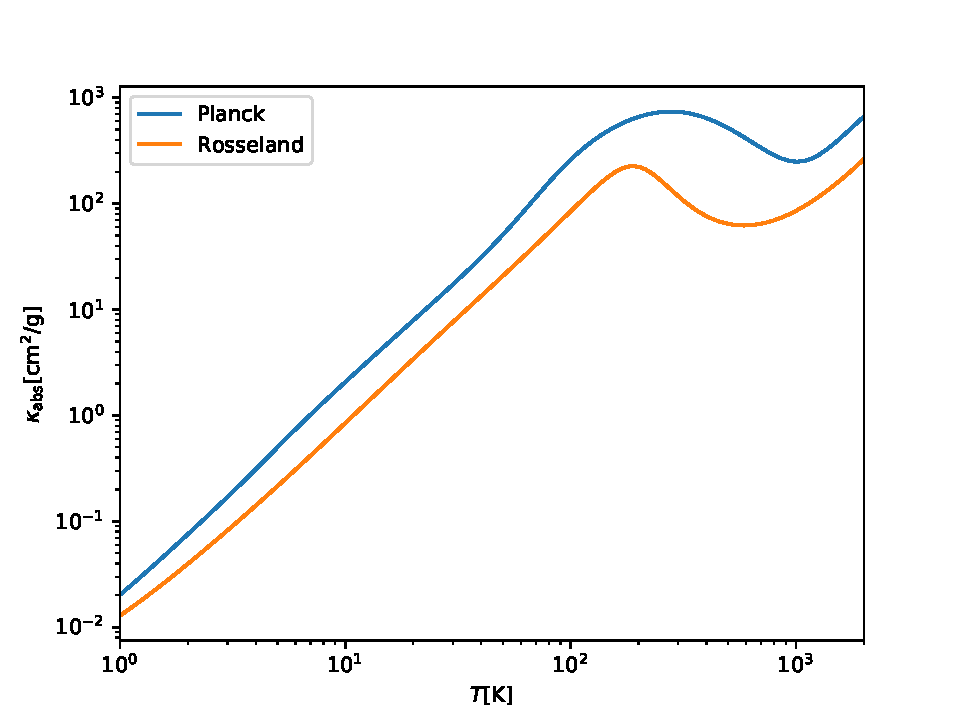
\includegraphics[width=0.7\textwidth]{../snippets/fig_snippet_plot_dustopac_2_1.pdf}}

{\em NOTE:} The dust opacity is the opacity {\em per gram of dust},
not per gram of gas+dust. So you have to beware of the proper
dust-to-gas ratio factor when using it in combination with the gas.

The computation of these mean opacities on run-time can be making
the code very slow. Therefore they are pre-computed and tabulated. This
is done by the method\\
\code{grain.tabulate\_mean\_opacities\_without\_sublimation()}. The
opacity reading methods \code{grain.read\_opacity()} and
\code{grain.load\_standard\_opacity()} both automatically call
this pre-computation method, so you do not have to call it yourself.
These pre-computed mean opacities are stored in the
\code{grain.meanopactable\_***} arrays.

The pre-computation of these tables is time-costly at startup. That is why the
first time you read in an opacity table, it will take a bit of time.  However,
{\sf DISKLAB} will write the table to file. The next time you read the opacity
file, the mean opacities will also be read from the previously computed
file. {\sf DISKLAB} will check if the tabulated mean opacities in this file are
still up-to-date with the wavelength-dependent opacity file from which it was
created. This is done using a hashing function SHA1 on the opacity file. Hence,
the second line of the file \code{dustkappa\_silicate.meanopac} is a hash, which
is the hash of the file \code{dustkappa\_silicate.inp}. If the hashes do not
match, the mean opacity table is recomputed.

Note that the mean opacities computed here are {\em without} sublimation.
Sublimation should be included by the appropriate reduction of the abundance
of this dust species. Some methods (such as the mean opacity methods of
Chapter \ref{chap-mean-opacities}) can do this automatically, but not all.




\chapter{Mean opacities for the disk model}
\label{chap-mean-opacities}
%
For computing the midplane temperature of the disk it is necessary to know the
Rosseland mean opacity and Planck mean opacity of the material of the disk.

{\bf Important:} In {\sf DISKLAB} the mean opacity and the frequency-dependent
opacity are (algorithmically speaking) independent from each other. The mean
opacities are only required for computing the disk interior (midplane)
temperature, and all the quantities that depend on that. The frequency-dependent
opacity is only used for computing the appearance of the disk at a given
frequency or wavelength. One {\em can} (and perhaps {\em should}) compute the
mean opacities from the wavelength-dependent ones, but from the perspective of
the {\sf DISKLAB} architecture, they are in principle independent, and serve
different purposes.

This chapter discusses the {\em mean} opacities.

The Rosseland- and Planck mean opacities are functions of gas density and
temperature, but not of wavelength or frequency (hence they are called {\em
  mean} opacities). For dust opacities they are only a function of temperature,
except when dust sublimation comes into play. Details about how one can
compute the mean opacities from the wavelength-dependent dust opacities
follow in Section \ref{sec-mean-opac-from-dust-opac}.

The mean opacities can vary from location to location. Not only because the
composition of the disk may vary from place to place (for instance, when
different dust grain components drift at different speeds), but also because of
the temperature and density dependence of the mean opacities themselves. At
radii $r$ close to the star, i.e.~in the hot regions of the disk, the mean
opacity of silicate dust will be very different from the mean opacity of the
same silicate dust in the disk cold outer regions (see Section
\ref{sec-mean-opac-from-dust-opac}).

A simple, yet flexible, implementation of the mean opacities is therefore not
trivial. The solution we have chosen in {\sf DISKLAB} is described in
Section \ref{sec-mean-opac-basic-architecture}. Various ways to compute
these opacities are described in the following sections.


\section{Basic architecture of mean opacity implementation}
\label{sec-mean-opac-basic-architecture}
%
At any moment in time, the Rosseland mean opacity as a function of
radius $r$ is (or better: should be) stored in the array
\begin{codebox}
d.mean_opacity_rosseland[:]
\end{codebox}
where \code{d} is the \code{DiskRadialModel} object. This is an array with the same
size as \code{d.r}, and it represents $\kappa_R$ at each of these
points. Likewise the Planck mean opacity $\kappa_P$ is stored in the array
\begin{codebox}
d.mean_opacity_planck[:]
\end{codebox}
As you can see: these values are given only as a function of $r$. The density
and temperature dependency is not explicitly stored here.

When \code{DiskRadialModel} needs $\kappa_P$ or $\kappa_R$ at a given radius $r$ (for
instance, to compute the midplane temperature, see Section
\ref{sec-irradiation-flaring-viscous-heating}), it will obtain these values from
\code{d.mean\_opacity\_planck[:]} and \code{d.mean\_opacity\_rosseland[:]}.

{\bf Important:} {\em You} (the user) will have to give \code{DiskRadialModel} the
command \code{compute\_mean\_opacity()} to compute the values of
\code{d.mean\_opacity\_planck[:]} and \code{d.mean\_opacity\_rosseland[:]}
according to some recipe. And you have to {\em re-}do this whenever the local
conditions in the disk change, which is, for instance, the case when you
viscously evolve the disk.

There are several ways by which \code{DiskRadialModel.compute\_mean\_opacity()} can
compute these values. To be more precise: {\sf DISKLAB} offers several {\em
  mean opacity models}:
\begin{itemize}
\item {\bf 'supersimple'} The simplest opacity model available: you simply specify
  a value to be used. See Section \ref{sec-mean-opac-supersimple}.
\item {\bf 'dustcomponents'} Self-consistently compute the mean opacities from
  the available dust components in the \code{d.dust} list. See Section
  \ref{sec-mean-opac-from-dust-opac}.
\item {\bf 'tabulated'} A user-provided 2-D table of $\kappa_R(\rho_g,T)$
  and $\kappa_P(\rho_g,T)$ values, for a discrete set of values of the
  gas density $\rho_g$ and temperature $T$.
\item {\bf 'belllin'} The famous Bell \& Lin (1994) opacity model.
\end{itemize}

The way to do this is to first set the \code{meanopacitymodel} variable of your
\code{DiskRadialModel} object. Let us take the \code{'supersimple'} model as an
example:
\begin{codebox}
from disklab.diskradial import *
from disklab.natconst import *
d=DiskRadialModel(mdisk=0.01*MS)
d.meanopacitymodel=['supersimple',{'dusttogas':0.01,'kappadust':1e3}]
d.compute_mean_opacity()
\end{codebox}
As you can see, the \code{d.meanopacitymodel} is a list. Its first element is
the name of the mean opacity model. The second element is a Python dictionary
with parameters for that mean opacity model.  All mean opacity models follow
this scheme (first element is name, second element is dictionary with
parameters).

For this 'supersimple' mean opacity model the values will be constant, independent
of the local conditions in the disk. However, for the other mean opacity models this
is not the case: whenever the disk changes (for instance, because it is viscously
evolving or photoevaporating or you name it), the mean opacities have to be
recalculated. This is done simply with
\begin{codebox}
d.compute_mean_opacity()
\end{codebox}

{\bf Important:} If you evolve the disk but forget to call \code{d.compute\_mean\_opacity()},
you are likely to get wrong results, especially if your model relies on proper values
of the mean opacities.

{\em Note:} In contrast to the dust opacities, the mean opacities for a disk
model are {\em cross-section per gram of gas}. For a gas+dust mixture, the
opacity is caused primarily by the dust, but the weighting is normalized to the
gas surface density. The reason for this is simple: if we are interested in
computing the midplane temperature, we are only interested in the vertical
optical depth, no matter if this is caused by dust or gas. Given that the disk
has only one gas component (\code{DiskRadialModel.sigma[:]}) but possibly multiple
dust components (\code{DiskRadialModel.dust[:].sigma[:]}), it makes life easier to
simply normalize the opacity to the gas surface density.


\section{The super-simple mean opacity model}
\label{sec-mean-opac-supersimple}
%
The super-simple mean opacity is simply a way to set the value of the mean
opacity to a number given by you. The simplest way is:
\begin{codebox}
d.meanopacitymodel = ['supersimple',{'kappagas':1e0}]
d.compute_mean_opacity()
\end{codebox}
You can also specify a hypothetical dust opacity, and a dust-to-gas
ratio:
\begin{codebox}
d.meanopacitymodel = ['supersimple',{'dusttogas':0.01,'kappadust':1e2}]
d.compute_mean_opacity()
\end{codebox}
(note that both examples give the same result).

You can also use this model to specify a r-dependent opacity,
simply by giving an array instead of a value:
\begin{codebox}
kappaarray         = np.ones_like(d.sigma)
d.meanopacitymodel = ['supersimple',{'kappagas':kappaarray}]
d.compute_mean_opacity()
\end{codebox}
where of course you set \code{kappaarray} to some more useful
array than just \code{np.ones\_like(d.rhogas)}, as long as it
has the same number of elements as \code{d.rhogas}.

The super-simple opacity model is, in fact, so simple, that you
could also do it by hand, without calling\\ \code{d.compute\_mean\_opacity()}:
\begin{codebox}
kappa = 0.01*1e3    # Dust-to-gas ratio 0.01 and dust kappa 1000
mean_opacity_planck[:] = kappa
mean_opacity_rosseland[:] = kappa
\end{codebox}

\section{Computing the mean opacities self-consistently from the dust opacities}
\label{sec-mean-opac-from-dust-opac}
%
\subsection{Basic method}
You can construct the mean opacity arrays from the available dust components in
the disk (or, instead, from the dust components you explicitly give as arguments
to this method). As usual, the \code{d.meanopacitymodel} consists of a list of
two elements, the first being \code{'dustcomponents'}, the second being a
dictionary with settings. The most important dictionary element is 'method'. It
can have the following values:
\begin{itemize}
\item {\bf 'fullcalculation':} Compute the mean opacities from the full
  frequency-dependent opacities of the dust components.  This model is very
  time-consuming, because it will recalculate the integrals over the full
  frequency grids.  For fast calculations of disk models, this is not ideal.
  But there can be circumstances by which this is the better method: if
  different dust species mix/drift in different ways, so that the composition of
  the dust mixture is different at different times.
\item {\bf 'simplemixing':} Use mean opacities from each of the dust species
  individually, and average them weighted by abundance.  For a single dust
  species this is of course exact.  For multiple dust species this is not quite
  correct, but it is fast. The reason why it is not quite correct is that the
  Rosseland mean of the mixed frequency dependent opacity is not equal to the
  average of the Rosseland mean of the individual dust opacities. It is only
  correct if the frequency- dependent opacities are 'correlated'. In atmospheric
  radiative transfer physics they call this the 'correlated k assumption'. It is
  the method of choice if one wants to allow time- and space- varying dust
  abundances, while avoiding the time- consuming 'fullcalculation' method.
\end{itemize}
Example:
\begin{codebox}
from disklab.diskradial import *
from disklab.natconst import *
d=DiskRadialModel(mdisk=0.01*MS)
d.add_dust(agrain=0.1,xigrain=2.0,dtg=0.005)
d.add_dust(agrain=0.01,xigrain=2.0,dtg=0.005)
for dust in d.dust:
   dust.grain.compute_simple_opacity()
d.meanopacitymodel = ['dustcomponents',{'method':'simplemixing'}]
d.compute_mean_opacity()
\end{codebox}
The call to \code{dust.grain.compute\_simple\_opacity()} computes the
simple dust opacity model of the Ivezic et al.~(1997) MNRAS 291, 121 paper,
and also (as a kind of 'bonus') computes a table of Planck and Rosseland
mean opacities for this single dust grain. The \code{'simplemixing'}
mean opacity method simply uses these tables to compute the mean opacities
for the full opacity model (i.e.~that of the dust mixture).

See Chapter \ref{chap-grain-model} for more information about dust opacities.

Let us do a more complex (and realistic) example: that of two standard grain
models: the 'astronomical silicate' model of Laor \& Draine (1993) ApJ 402, 441,
and 'amorphous carbon' measurements of Preibisch et al.\ (1993) A\&A 279, 577.
These are two of the opacity models from the disk modeling paper of Dullemond,
Dominik \& Natta (2001) ApJ 560, 957, hence the name \code{ddn01}.
\begin{codebox}
from disklab.diskradial import *
from disklab.natconst import *
d=DiskRadialModel(mdisk=0.01*MS)
d.add_dust(agrain=0.1e-4,xigrain=3.6,dtg=0.005)
d.add_dust(agrain=0.1e-4,xigrain=1.8,dtg=0.005)
d.dust[0].grain.load_standard_opacity('ddn01','silicate')
d.dust[1].grain.load_standard_opacity('ddn01','carbon')
for dust in d.dust:
   assert dust.grain.agrain==dust.agrain.max()
   assert dust.grain.xigrain==dust.xigrain.max()
d.meanopacitymodel = ['dustcomponents',{'method':'simplemixing'}]
d.compute_mean_opacity()
\end{codebox}
The \code{assert} statements are meant to make sure that the \code{agrain} and
\code{xigrain} we specify for the disk components are the same as those of the
precalculated standard dust opacities. This is because the
precalculated standard dust opacities have a fixed grain size and material
density. Using these opacities for a dust component with different grain size
or material density would be physically inconsistent. In the above example
these \code{assert} statements are, of course, passed succesfully.

The \code{'fullcalculation'} method can be compared to the \code{'simplemixing'}
\begin{codebox}
kapros_simple = d.mean_opacity_rosseland.copy()
d.meanopacitymodel = ['dustcomponents',{'method':'fullcalculation'}]
d.compute_mean_opacity()
kapros_full = d.mean_opacity_rosseland.copy()
\end{codebox}
These two are usually not much different, showing that in most cases
the \code{'simplemixing'} method is accurate enough.

\subsection{Including sublimation physics}
When including dust species that can easily sublimate (e.g.\ ices), it is
imperative to include the sublimation physics. The location where this phase
transition occurs is often called the 'ice line'. In fact, even silicate or
carbon dust will sublimate at high enough temperatures. Simply computing the
mean opacities without taking into account this sublimation would yield
unphysical mean opacities.

The sublimation and freeze-out physics is included in the \code{GrainModel}
class and is described in Section \ref{sec-sublimation-and-freezeout}.  By
default this is not included in the computation of the mean opacities.  If you
wish to include the sublimation and freeze-out in the computation of the mean
opacities, you have to explicitly activate this. Either you reduce the dust
component surface densities youself according to the methods described in
Section \ref{sec-sublimation-and-freezeout} (this requires a bit of
tinkering on your side), or you can let \code{compute\_mean\_opacity()} do
it automatically for you, which is done with the \code{'autosublim'}, as in:
\begin{codebox}
d.meanopacitymodel = ['dustcomponents',{'method':'simplemixing','autosublim':True}]
\end{codebox}
{\em Note:} If you use the \code{'autosublim':True}, then
\code{d.compute\_mean\_opacity()} interprets the dust component surface
densities \code{d.dust[:].sigma} as the {\em combined dust+vapor surface
  density}. So it depends on your modeling goals whether you use the easy-to-use
automatic \code{'autosublim':True} method, or whether you instead handle the
dust and vapor as separate dust components and implement the sublimation physics
directly as a source/sink exchange term between these components using the
sublimation physics routines of Section \ref{sec-sublimation-and-freezeout}.

\subsection{When all the dust is gone: Gas opacity model of Bell \& Lin}
For very hot regions of the disk, all dust will be sublimated. When we
compute the mean opacities from the dust components in the disk, this
would mean that the mean opacity will drop to zero. This can cause
problems for the model, and is also not very realistic. To ameliorate
this, you can ask the mean opacity model to add the {\em gas-opacity part}
of the Bell \& Lin (1997) opacities (see Section \ref{sec-mean-opac-bellin})
to be added. When the dust is gone, the gas opacities remain. This can
be done by adding \code{'gasbelllin':True} like this:
\begin{codebox}
d.meanopacitymodel = ['dustcomponents',{'method':'simplemixing', \
                      'autosublim':True,'gasbelllin':True}]
\end{codebox}

\subsection{Let us plot some of these mean opacity models}\label{sec-opacity-models}
Let us give a few examples of how these mean opacities look. Let us make a disk
model around a Herbig star with $M_{*}=2*M_{\odot}$, $T_{*}=10^4$ K, and
$L_{*}=30*L_{\odot}$, including olivine and water ice dust, and plot the various
approximations of the mean opacities. We also overplot the full Bell \& Lin
opacity of Section \ref{sec-mean-opac-bellin}.

The code snippet is
\code{snippet\_plot\_dustopac\_5.py}. In Python run it as:
\begin{codebox}
%run snippet_plot_dustopac_5.py
\end{codebox}
Here is the listing:
\lstinputlisting{../snippets/snippet_plot_dustopac_5.py}
\centerline{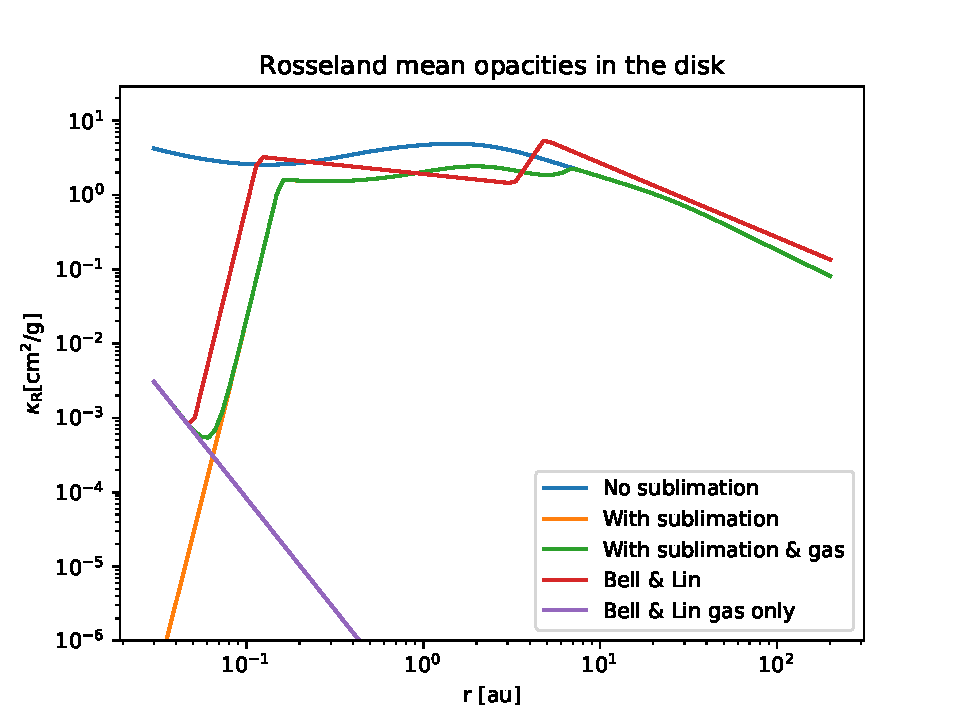
\includegraphics[width=0.7\textwidth]{../snippets/fig_snippet_plot_dustopac_5_1.pdf}}

Here we have chosen a powerlaw smoothing of the olivine sublimation front of
$-24$, consistent with the Bell \& Lin opacity. For the water snow line
(the H$_2$O sublimation) we have chosen the powerlaw less steep (more smooth):
$-10$, which accounts for the gentle opacity transition near the snow line
around 7 au. Remember that more gentle snow line phase transitions are
easier for a numerical code to handle.

{\em Note:} This disk model does {\em not} include the ``dust inner rim'' (see
Dullemond, Dominik \& Natta 2001 ApJ 560, 957). See Section
\ref{sec-dust-inner-rim} for some notes about the dust inner rim.  In the above
model the dust sublimation radius is around 0.1 au.  If we would include the
inner rim physics, then the sublimation of dust would probably move to a larger
radius (see Dullemond, Dominik \& Natta 2001 ApJ 560, 957).

Perhaps it would be nicer to plot the mean opacities as a function of
temperature. Let us do this here, for a gas density of
$\rho_{\mathrm{gas}}=10^{-10}\,\mathrm{g}/\mathrm{cm}^3$. We can make
direct use of the routines in \code{meanopacity.py} (which are used
by \code{diskradial.py}).

The code snippet is
\code{snippet\_plot\_dustopac\_6.py}. In Python run it as:
\begin{codebox}
%run snippet_plot_dustopac_6.py
\end{codebox}
\centerline{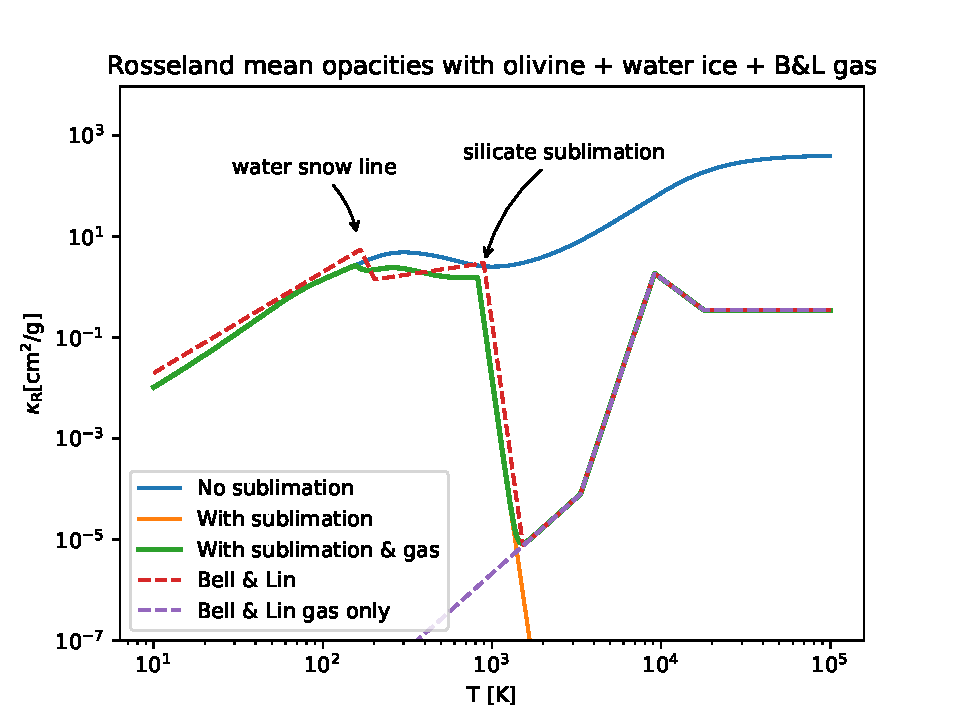
\includegraphics[width=0.7\textwidth]{../snippets/fig_snippet_plot_dustopac_6_1.pdf}}

You can see that the opacity jump at the water snow line is much weaker than
for the Bell \& Lin opacity model. This is because Bell \& Lin chose
a water ice abundance that is much higher than the 50\% by mass that
we take in our calculations.


\section{Tabulated mean opacities}
\label{sec-mean-opac-tabulated}
%
{\sf DISKLAB} allows the user not only to include mean opacities from prescribed
mean opacity models, but also allows the user to provide a completely
user-defined table of mean opacities. The user should provide a table of
$\kappa_P(\rho_{g},T)$ and $\kappa_R(\rho_{g},T)$ for a rectangular grid in the
variables $\rho_g$ and $T$.

Here is an example. Suppose we wish to implement Kramer's free-free opacity law:
\begin{equation}
\kappa_{\mathrm{ff}} = 3.68\times 10^{22}g_{\mathrm{ff}}(1-Z)(1+X)\rho_{g}T^{-7/2}
\end{equation}
which is the Rosseland mean. We take it, for convenience, also for
the Planck mean. Here is how we implement it:
\begin{codebox}
from disklab.diskradial import *
from disklab.natconst import *
d       = DiskRadialModel(mdisk=0.01*MS)
rhogas0 = 1e-20
rhogas1 = 1e-5
nrhogas = 5
rhogas  = rhogas0 * (rhogas1/rhogas0)**np.linspace(0.,1.,nrhogas)
temp0   = 1.e3
temp1   = 1.e6
ntemp   = 5
temp    = temp0 * (temp1/temp0)**np.linspace(0.,1.,ntemp)
rhog2d, temp2d = np.meshgrid(rhogas, temp, indexing='ij')
Z       = 0.
X       = 1.
gff     = 1.
kappa   = 3.68e22*gff*(1.-Z)*(1.+X)*rhog2d*temp2d**(-7./2.)
ln_kappa= np.log(kappa)
method  = 'linear'
d.meanopacitymodel = ['tabulated',{'rhogrid':rhogas,'tempgrid':temp, \
                                   'ln_kappa_planck':ln_kappa,       \
                                   'ln_kappa_rosseland':ln_kappa,    \
                                   'method':method}]
d.compute_mean_opacity()
\end{codebox}
The code until and including \code{kappa} is creating the 2-D table of mean
opacity according to the Kramer's formula. We use here only a very coarse grid:
5 points in density and 5 points in temperature.  If we would use linear
interpolation in such a table, given that Kramer's opacity is very strongly
dependent on temperature, we would get very bad interpolated values. However, by
specifying \code{'ln\_kappa\_planck'} and \code{'ln\_kappa\_rosseland'} instead
of \code{'kappa\_planck'} and \code{'kappa\_rosseland'} (which we could have
done as well), we tell \code{compute\_mean\_opacity()} to do the interpolation
with the logarithm of the values instead of with the actual values. Such
log-interpolation is much more robust for functions that vary over many
orders of magnitude. Hence we use this here.

Do not forget to call \code{d.compute\_mean\_opacity()} again, every
time that \code{d.tmid[:]} or \code{d.sigma} changes. And if
\code{d.sigma} changes, you must recompute \code{d.rhomid} using
\code{d.compute\_rhomid\_from\_sigma()}, because it is \code{d.rhomid}
(together with \code{d.tmid}) that enter into the opacity calculation.

{\em Note:} The phrasing ``tabulated mean opacity'' is used in different
contexts. In Chapter \ref{chap-grain-model}, where the wavelength-dependent
opacities of dust grains are discussed, the mean opacities are computed
self-consistently (see also Section \ref{sec-mean-opac-from-dust-opac}), and --
for speed -- are also precalculated, tabulated and even written to a file. In
contrast, the ``tabulated mean opacity'' used in this section are meant mostly
for user-specified tables of mean opacities.


\section{Bell \& Lin mean opacities}
\label{sec-mean-opac-bellin}
%
Among disk radiation hydrodynamics modellers the opacity model of Bell \& Lin
(1994) ApJ 427, 987 is very popular. It is a simple analytic opacity model
consisting of several powerlaw segments stitched together.  It is valid for high
temperatures, when the dust has vanished through sublimation, as well as for
lower temperatures, where dust is present.

Using this opacity model as Planck- and Rosseland-mean opacity in {\sf
  DISKLAB} is easy:
\begin{codebox}
from disklab.diskradial import *
from disklab.natconst import *
d=DiskRadialModel(mdisk=0.01*MS)
d.meanopacitymodel = ['belllin']
d.compute_mean_opacity()
\end{codebox}
Do not forget to call \code{d.compute\_mean\_opacity()} again, every
time that \code{d.tmid[:]} or \code{d.sigma} changes. And if
\code{d.sigma} changes, you must recompute \code{d.rhomid} using
\code{d.compute\_rhomid\_from\_sigma()}, because it is \code{d.rhomid}
(together with \code{d.tmid}) that enter into the opacity calculation.

Note that the Bell \& Lin opacity table includes a gas-part and a dust-part.
The dust part is valid only for the dust and ice abundances assumed by
the Bell \& Lin paper. It may not be consistent with the dust abundances
you have in your model! You can choose the gas-only part by setting
\begin{codebox}
d.meanopacitymodel = ['belllin',{'onlygas':True}]
\end{codebox}
Or if you wish to simply reduce the dust content, you can do this
by setting
\begin{codebox}
d.meanopacitymodel = ['belllin',{'dustfactor':0.02}]
\end{codebox}
which reduces the dust content by a factor of 50 in this example.
An example of Bell \& Lin opacities with reduced dust content is
given by snippet
\code{snippet\_plot\_meanopac\_belllin\_1.py}. In Python run it as:
\begin{codebox}
%run snippet_plot_meanopac_belllin_1.py
\end{codebox}
\centerline{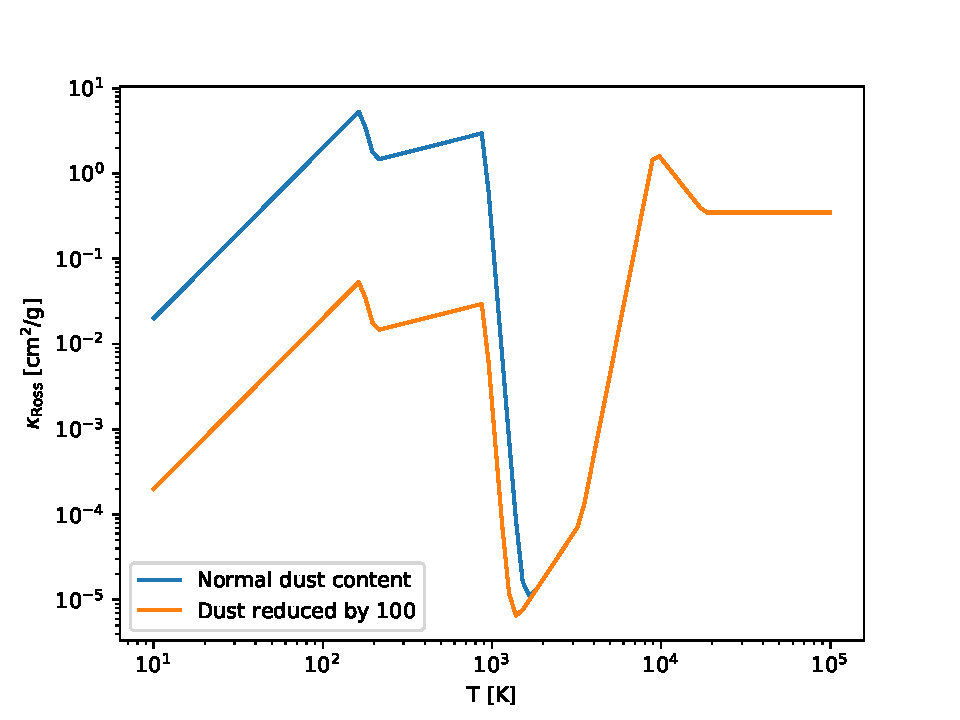
\includegraphics[width=0.7\textwidth]{../snippets/fig_snippet_plot_meanopac_belllin_1_1.pdf}}


{\em Note:} The Bell \& Lin dust opacity in this model is, however, very
simplified. And there is no wavelength-dependent version of these
opacities. That means that any post-processing of these models with
wavelength-dependent radiative transfer (for instance, the RADMC-3D code) to
obtain synthesized observations, will be difficult with the Bell \& Lin
model. Some modellers take radiation-hydrodynamics models made with the Bell \&
Lin opacities, and then post-process these with entirely different dust
opacities for comparison to observations. This can be problematic. It is
therefore perhaps more self-consistent to use the actual dust opacities (see
Section \ref{sec-mean-opac-from-dust-opac} and Chapter \ref{chap-grain-model}).
It is even possible to add the gas-only part of the Bell \& Lin opacities
to those dust opacities, to get more self-consistency.


\section{Application of the mean opacities}
%
This chapter dealt with the {\em mean} opacities of the disk. When are they
necessary? They are necessary primarily for the computation of the disk thermal
structure. The thermal structure, in turn, affects the disk vertical structure
as well as the viscous evolution, though in both cases the effects are only
moderate. The vertical scale height of the disk is ``only'' dependent on the
square-root of the temperature, and the viscous evolution depends ``only''
linearly on temperature.

But let us experiment with the effect of such ``realistic'' mean opacities
on the disk flaring and midplane temperature.






{\bf TO BE DONE: Flaring 1D, viscous heating.}







\chapter{Simple radiative transfer model for computing (sub-)millimeter appearance}
To compute how a protoplanetary disk looks at different wavelengths is a rather
complex problem. It requires, in general, a full-fledged radiative transfer code
such as the \code{RADMC-3D} code or similar codes (see Chapter
\ref{chap-links-to-external-codes}).

However, for some cases one can make simple estimates without having to resort
to the full-scale radiative transfer computation. This is, for instance, the
case for thermal emission calculations in the millimeter wavelength regime. As
long as the wavelength is long enough to be in the Rayleigh-Jeans regime of the
Planck spectrum for the given disk midplane temperature, the resulting emission
is not too sensitive to inaccuracies in the radiative transfer algorithm.

Let us make a simple estimate: Let us assume that the lowest temperature in the
disk midplane is 10 K. The peak of the Planck curve is at about $\nu\simeq
3k_BT/h$, which is is about 625 GHz, or 0.5 millimeter wavelength. That means
that for ALMA band 6 ($\lambda\simeq 1.3\,\mathrm{mm}$) we are moderately in the
Rayleigh-Jeans regime.  The difference between $B_\nu(T)$ at $T=10\,\mathrm{K}$
and $T=20\,\mathrm{K}$ at this wavelength is a factor of 2.7, meaning that an
error of a factor of 2 in our estimate of the temperature leads ``only'' to an
error of a factor or 2.7 in the thermal emission. However, for ALMA band 9
($\lambda\simeq 0.4\,\mathrm{mm}$), the difference between $B_\nu(T)$ at
$T=10\,\mathrm{K}$ and $T=20\,\mathrm{K}$ is a factor of 6.4, meaning that an
error of a factor of 2 in our estimate of the temperature now leads to an
error of a factor or 6.4 in the thermal emission.

What should we conclude from this? It means that when we study protoplanetary
disks with longer wavelengths than about 1 mm (e.g.\ with the VLA), we are safe
with the simple one-zone radiative transfer models that we will describe in this
section. Also for ALMA bands it is ok, although for ALMA's higher-frequency
bands we are on the border of the reliability of such simple radiative transfer
models. For shorter wavelengths (far-infrared all the way down to the optical),
however, there is no reliable simple radiative transfer recipe, and we are
forced to use full radiative transfer tools such as \code{RADMC-3D}.

In the present section we will therefore describe a simple one-zone radiative
transfer model that can be used for ALMA and VLA (and similar radio telescopes),
but not for shorter wavelengths.


\section{Specifying the wavelength-dependent dust opacity}
\label{sec-simple-dust-opacity}
For computing thermal dust emission from a disk we first need to have a model
of the wavelength-dependent dust opacity. Such dust opacities are handled by
the \code{GrainModel} class (see Chapter \ref{chap-grain-model}). Each dust
component of the disk (\code{d.dust[0]}, \code{d.dust[1]}, ..., depending how
many dust components you have added to the disk model \code{d}) should have
its own grain model. You can check this:
\begin{codebox}
from disklab.diskradial import *
from disklab.natconst import *
d = DiskRadialModel(mdisk=0.01*MS)
d.add_dust(agrain=1e-4,xigrain=3.6,dtg=0.1)
d.dust[0].grain
Out[]: <disklab.grainmodel.GrainModel at 0x10a82eb10>
\end{codebox}
In this example, since we specified \code{agrain} when calling
\code{d.add\_dust()}, such a grain model was automatically added to the dust
component. If you specify, instead of \code{agrain}, the Stokes number
\code{St}, then such a grain model will not be automatically added:
\begin{codebox}
from disklab.diskradial import *
from disklab.natconst import *
d = DiskRadialModel(mdisk=0.01*MS)
d.add_dust(St=0.1)
d.dust[0].grain
---------------------------------------------------------------------------
AttributeError                            Traceback (most recent call last)
<ipython-input-6-8227c413dfd4> in <module>()
      3 d = DiskRadialModel(mdisk=0.01*MS)
      4 d.add_dust(St=0.1)
----> 5 d.dust[0].grain

AttributeError: 'DiskRadialComponent' object has no attribute 'grain'
\end{codebox}
The reason is simply that in this case there is no single grain size associated
to this dust component, so no single grain model can be associated with it.

But let us go back to the first example, where we set \code{agrain=1e-4} (i.e.\ we
specified the grain radius to be 1 $\mu$m), and a grain model is automatically
associated to the dust component.

We can now ask the grain model object \code{d.dust[0].grain} to produce a simple
analytic dust opacity for us.
We do this by calling the method \code{grain.compute\_simple\_opacity()} and
specify a wavelength:
\begin{codebox}
lam = 0.13     # Wavelength 1.3 mm, which lies within band 6 of ALMA
d.dust[0].grain.compute_simple_opacity(lam)
\end{codebox}
This produces the following data:
\begin{codebox}
d.dust[0].grain.opac_lammic
Out[]: array([ 1300.])
d.dust[0].grain.opac_kabs
Out[]: array([ 10.06920722])
\end{codebox}
which means that the dust opacity has been calculated to be
$\kappa_{\mathrm{abs},\nu}=10.069\,\mathrm{cm}^2/\mathrm{g}$, which is {\em per gram
  of dust}. The optical depth of the disk is defined as
\begin{equation}
  \tau_\nu(r) = \Sigma_{\mathrm{dust}}(r) \kappa_\nu^{\mathrm{abs}}
\end{equation}
So for our model (assuming that \code{d.dust[0]} is the only
dust component) this would then be:
\begin{codebox}
taudisk = d.dust[0].sigma * d.dust[0].grain.opac_kabs[0]
\end{codebox}
If you have multiple dust components:
\begin{codebox}
lam = 0.13     # Wavelength 1.3 mm, which lies within band 6 of ALMA
tau = np.zeros_like(d.sigma)
for dust in d.dust:
   dust.grain.compute_simple_opacity(lam)
   tau += dust.sigma * dust.grain.opac_kabs[0]
\end{codebox}

\section{One-zone radiative transfer model for dust emission}
\label{sec-simple-radtrans}
Once a dust opacity is set, you can compute the emerging intensity from the disk,
assuming face-on inclination, and assuming a one-zone model (i.e.\ no ``warm
surface layer''). This is computed using the method\\ \code{compute\_onezone\_intensity()}:
\begin{equation}
I_\nu(r) = \left(1-\exp(-\tau_\nu(r))\right)\,B_\nu(T)
\end{equation}
where $B_\nu(T)$ is the Planck function in the usual CGS units of
erg/cm$^2$/s/Hz/ster.  This is stored in \code{intensity}. One can also express
the intensity as a brightness temperature using
\code{compute\_tbright\_from\_intensity()}.

Example. The code snippet is
\code{snippet\_simple\_rt\_2.py}. In Python run it as:
\begin{codebox}
%run snippet_simple_rt_2.py
\end{codebox}
Here is the listing:
\lstinputlisting{../snippets/snippet_simple_rt_2.py}
\centerline{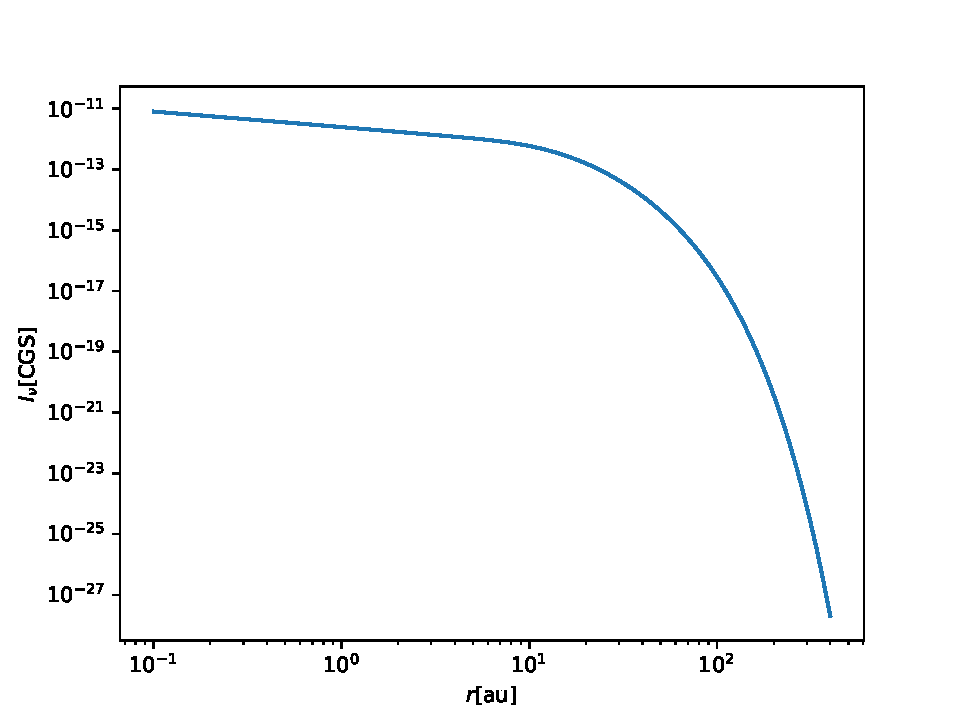
\includegraphics[width=0.5\textwidth]{../snippets/fig_snippet_simple_rt_2_1.pdf}
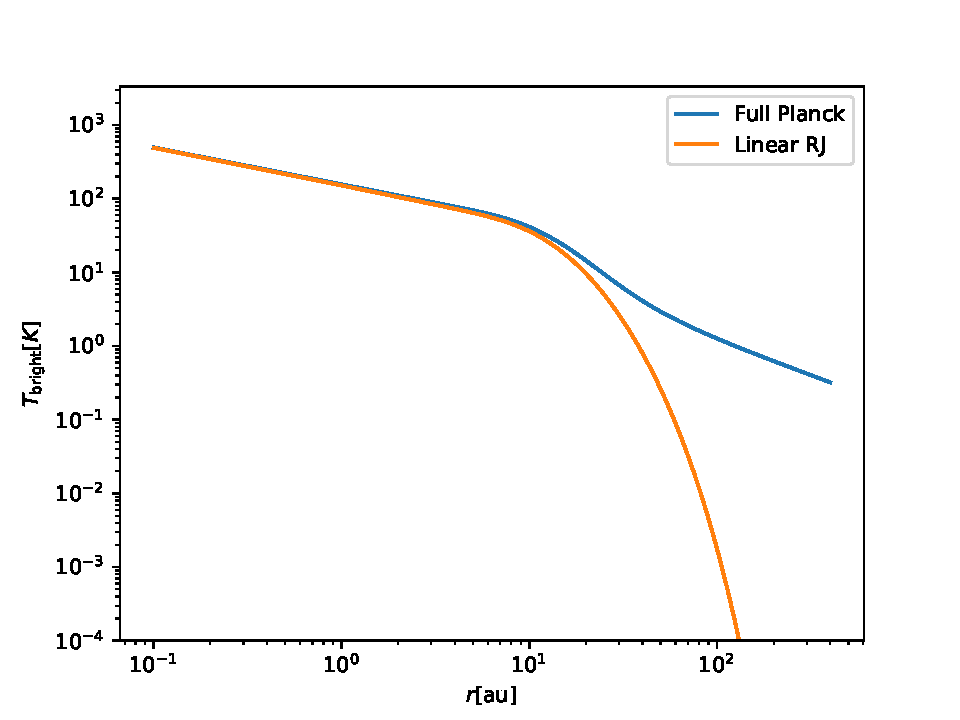
\includegraphics[width=0.5\textwidth]{../snippets/fig_snippet_simple_rt_2_2.pdf}}

\section{Including ``real'' dust opacities}\label{sec-incl-real-dust-opac}



{\bf [TIL: WILL YOU WORK ON THE REAL OPACITY MODEL?]}



So far we simply ``guessed'' the dust opacity. But the \code{GrainModel}
class has methods for
reading dust opacity data. In the \code{opacity/} directory there is
a file called \code{dustkappa\_silicate.inp} (a copy of which is also
in the \code{snippets/} directory).





{\bf MOVE THIS STUFF}












{\bf INCLUDE HOW TO INCLUDE SUBLIMATION}




\chapter{Advanced applications of the DiskRadialModel class}
Here we give a few more sophisticated examples of how the \code{DiskRadialModel} class
can be used to solve problems in astrophysics. All these models are stand-alone
code snippet files that can be run from within Python using the \code{\%run}
command with the snippet file name. Or you can directly call Python from the
command line with the code snippet file name added.

\section{Radial mixing of crystalline silicates}
A model of full disk evolution with a massless dust component passively moving
along, but continously set to the dust-to-gas ratio inward of the point where the
temperature is higher than the crystallization temperature. The code snippet is
\code{snippet\_radialmix\_crystals\_1.py}. In Python run it as:
\begin{codebox}
%run snippet_radialmix_crystals_1.py
\end{codebox}
Here is the listing:
\lstinputlisting{../snippets/snippet_radialmix_crystals_1.py}
\centerline{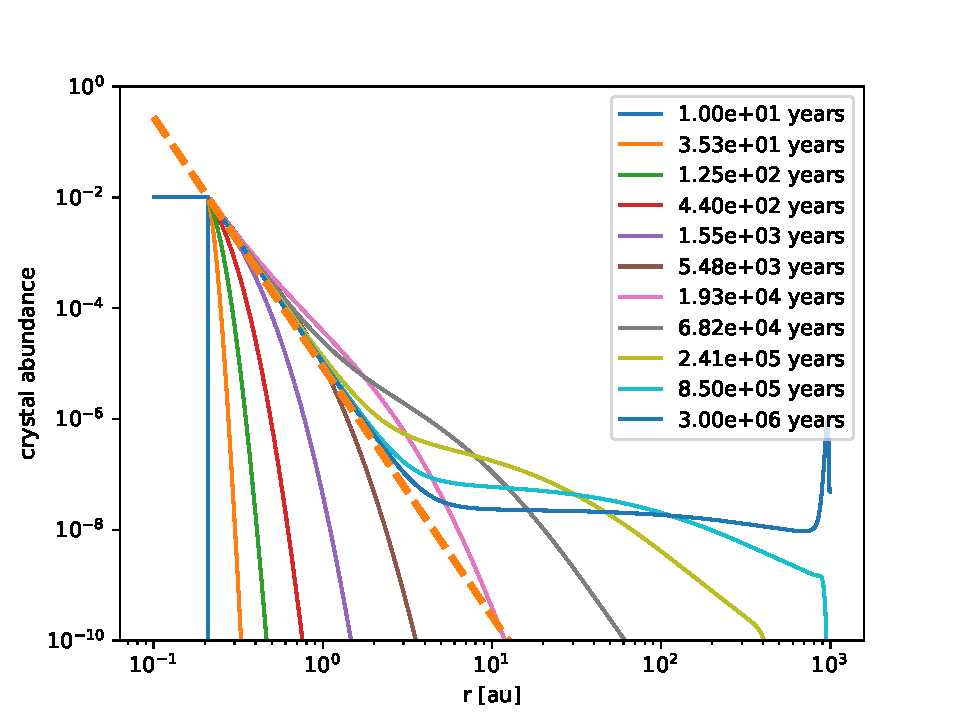
\includegraphics[width=0.7\textwidth]{../snippets/fig_snippet_radialmix_crystals_1_1.pdf}}
The different lines are different time snapshots, with logarithmic time intervals.

The crystallization is implemented directly inside the implicit differencing code.
We make use of the ``internal condition'' method, where we replace the differential
equation with a condition similar to a boundary condition. We do this at the largest
radius where the $T>T_{\mathrm{cryst}}$. That is sufficient, because inside of that point
everything has passed through that point (except at the very beginning, which is why
at the start we ``crystallize'' by hand).

Overplotted as a dashed line is the analytic powerlaw from Clarke \& Pringle (1988)
MNRAS 235, 365 (see also Pavlyuchenkov \& Dullemond 2007, A\&A 471, 833). Note that
to obtain the correct powerlaw (as shown in this example), the model requires indeed
about 1000 radial gridpoints (i.e.\ 250 gridpoints per decade in radius). With 100
gridpoints, as you can verify yourself, you will find that the mixing is too strong.

Another thing that can be seen is that there is a period where the mixing outward
appears to be more efficient that the analytic slope. That is because the whole disk
is still expanding in this early phase.

Note that the example of crystalline sillicates mixing here is done with {\em one}
dust species. But this can be also done with the multi-dust-species methods
(see Section \ref{sec-multi-dust-spec}). So let's do {\em exactly the same} but
now with the multi-species method. The code snippet is
\code{snippet\_radialmix\_crystals\_2.py}. In Python run it as:
\begin{codebox}
%run snippet_radialmix_crystals_2.py
\end{codebox}
Here is the listing:
\lstinputlisting{../snippets/snippet_radialmix_crystals_2.py}
We do not show the plot, because it is exactly the same as above. The advantage of
the multi-species version of this code snippet is that this one is easier to
generalize to many-species models. For instance, if you want to do more complex
chemistry of the dust in the disk.

\subsection{Crystallization: Why not use operator-splitting?}
We implemented the crystallization condition inside the implicit differencing
code for the transport (=mixing and drift). Why? Wouldn't it be much more
straightforward to use the method of 'operator splitting'? Operator splitting is
the method in which different processes happening at the same time in reality
are handled one-after-the-other in the numerical scheme. Here we could consider
doing the dust mixing step first, and then make all the dust crystalline where
the temperature is higher than 800 K, and then continue to the next time step,
where we again first to transport, then crystallization. Let us try this out
and see what happens. Let us replace in the above examples the
internal condition with simply setting the dust to crystalline in the inner
(hot) regions. The code snippet is \code{snippet\_radialmix\_crystals\_3.py}. In
Python run it as:
\begin{codebox}
%run snippet_radialmix_crystals_3.py
\end{codebox}
Here is the listing:
\lstinputlisting{../snippets/snippet_radialmix_crystals_3.py}
\centerline{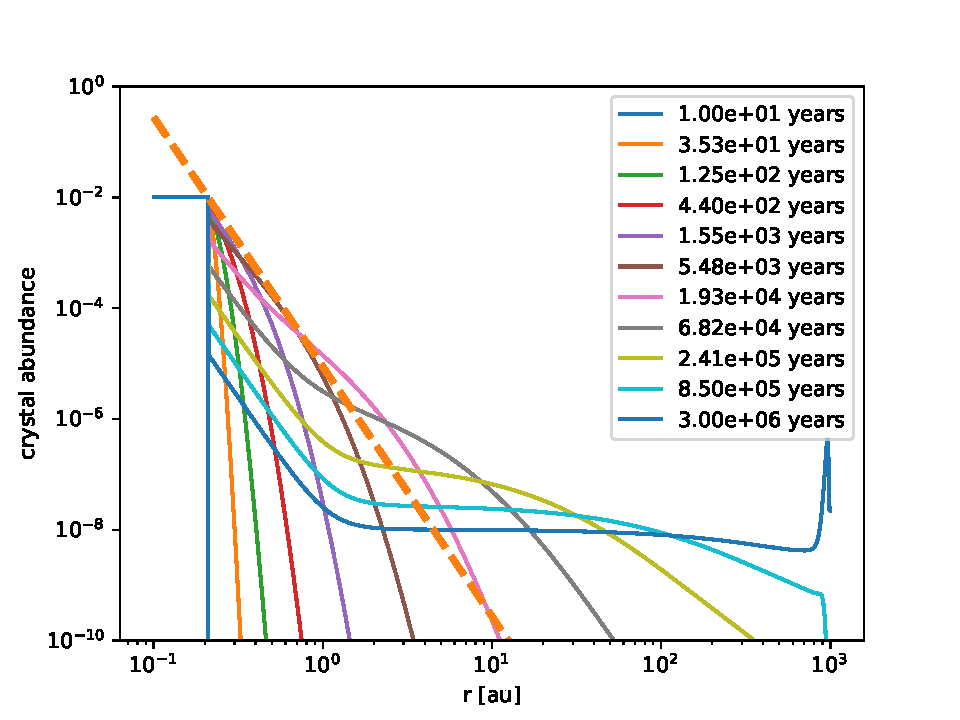
\includegraphics[width=0.7\textwidth]{../snippets/fig_snippet_radialmix_crystals_3_1.pdf}}
You can see that the results are strange: the crystal-abundance makes a jump
right after the crystallized part. This is clearly not correct. Let us analyze
why.

The operator splitting method would work fine {\em if} we use small enough time
steps. The time step must be small enough that the mixing step does not change
the dust surface density by more than a few tens of percent at most. Or to put
it more scientifically: The time step must obey the Courant-Friedrichs-Lewy
(CFL) condition. Then the transport and the crystallization both modify the dust
only by modest amounts and the results will be reasonably accurate.

However, because we use a super-stable transport scheme (implicit differencing)
we usually take super-large time steps. At the end of the model the time steps
are about a 1000$\times$ larger than the CFL condition at the inner edge of the
disk. If the transport scheme were an explicit differencing scheme, the model
would have already blown up long ago. By virtue of the implicit differencing
the radial drift and mixing method still works stably for these super-large
time steps.

However, if we add new physics (here: crystallization) using the
operator-splitting method (and thus not included in the implicit integration
scheme), then the implicit drift-and-mixing method will not treat this
physics. For the entire time step it thinks that this physics is not
included. Only at the end of the time step, when the crystallization is carried,
the inner disk is re-crystallized. However, by then the implicit differencing
time step has already shifted almost all the crystals into the inner boundary.
This means that the way we calculate the abundance of crystals is no longer
accurate. {\em This is therefore an example of how the radial mixing and drift
  calculations can go wrong if not done carefully}.

One solution (other than using the internal condition) could be to use
very small time steps. But that is of course numerically very costly.

The problem we demonstrate here is a general problem when using an implicitly
differenced transport scheme in combination with another method in an
operator-splitted way (one step transport, one step other method, then one step
transport again and one step other method again etc). One can only take large
time steps if one does {\em all} the processes within a single implicit scheme.

This becomes tricky if you couple radial drift and mixing of a multi-dust-species
problem to chemistry. The chemistry may couple the various dust species to each
other at each location, while the transport will move them around. How can this
be done? Typically it would simply mean that you would have to reduce the time
step enormously (and thus increase the computational cost enormously). If the
chemistry rates are small enough (i.e.\ the chemical time steps are long enough)
then you only have to ensure that the time steps are small enough to handle the
chemistry explicitly. But at any rate: the time steps may become substantially
smaller than we usually use.


\pagebreak
\section{Ring-shaped dust traps}
In the paper by Pinilla, Birnstiel, Ricci, Dullemond, Uribe, Testi, \& Natta
(2012) A\&A 538, 114, a simple bumpy disk model was implemented to see how
the dust could be trapped by these bumps. That model also included the
dust coagulation. Let us here do something similar, but without the dust
growth. First, we want to make a ``sine wave'' with varying wavelength,
such that the local wavelength is always a constant factor $\zeta$ times
the local pressure scale height:
\begin{equation}
\lambda_{\mathrm{wave}}(r) = \zeta H_p(r)
\end{equation}
We can numerically compute the phase $\Phi(r)$ by numerical integration of
the following equation:
\begin{equation}
\frac{d\Phi(r)}{dr} = \frac{2\pi}{\lambda_{\mathrm{wave}}(r)}
\end{equation}
which gives:
\begin{equation}
\Phi(r) = \Phi_0 + \int_{\mathrm{r_0}}^r \frac{2\pi}{\lambda_{\mathrm{wave}}(r')}dr'
\end{equation}
The wave is then the following dimensionless function:
\begin{equation}
w(r) = A \sin\left(\Phi(r)\right)
\end{equation}

We could use this directly for making the surface density profile:
\begin{equation}
\Sigma_g(r) = \Sigma_{g1}(r)\,(1+w(r))
\end{equation}
where $\Sigma_{g1}(r)$ is the unperturbed surface density from one of the
models of Chapter \ref{chap-standard-disk-models}. However, if we then let
the disk viscously evolve, the bumps will quickly disappear again.

Instead we apply the wave to the viscosity. To allow experimentation with large
amplitudes, we apply it in log-space, i.e.\ we add it to $\ln\nu(r)$, or
equivalently to $\ln\alpha(r)$:
\begin{equation}
\ln\alpha(r) = \ln\alpha_1(r) + A \sin\left(\Phi(r)\right)
\end{equation}
where $\alpha_1(r)$ is the unperturbed value of $\alpha$, which is usually
taken to be constant with $r$ but could equally well be $r$-dependent.

Here is a setup example. We use the combined gas and dust evolution method
of \code{DiskRadialModel}. The code snippet is
\code{snippet\_rings\_dusttrap\_1.py}. In Python run it as:
\begin{codebox}
%run snippet_rings_dusttrap_1.py
\end{codebox}
Here is the listing:
\lstinputlisting{../snippets/snippet_rings_dusttrap_1.py}
\centerline{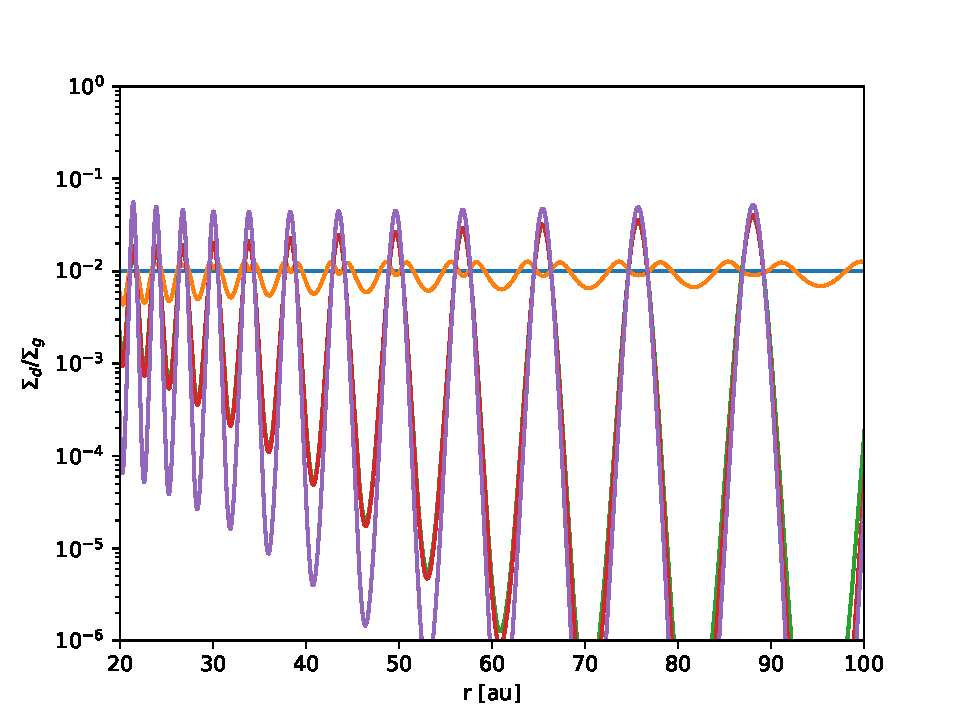
\includegraphics[width=0.5\textwidth]{../snippets/fig_snippet_rings_dusttrap_1_1.pdf}
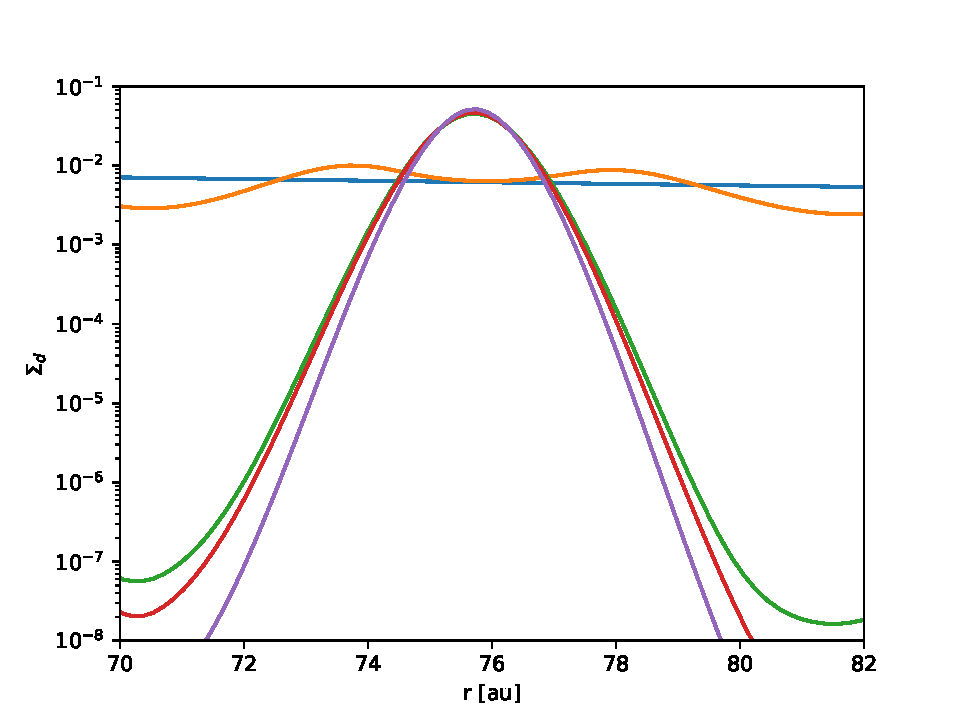
\includegraphics[width=0.5\textwidth]{../snippets/fig_snippet_rings_dusttrap_1_2.pdf}}
In the first figure the dust-to-gas ratio is shown. This model shows how the
dust gets trapped and concentrated in to thin rings. In the second figure a
zoom-in on one of these rings is shown, this time the actual dust surface
density


\pagebreak
\section{Simple planetary gap model with dust drift}
A simple model of a gap produced by a planet is presented by Duffell (2015) ApJL
807, 11. Let us see how the dust drift reacts to that. The code snippet is
in \code{snippet\_planetgap\_dustdrift\_1.py}. In Python run it as:
\begin{codebox}
%run snippet_planetgap_dustdrift_1.py
\end{codebox}
Here is the listing:
\lstinputlisting{../snippets/snippet_planetgap_dustdrift_1.py}
\centerline{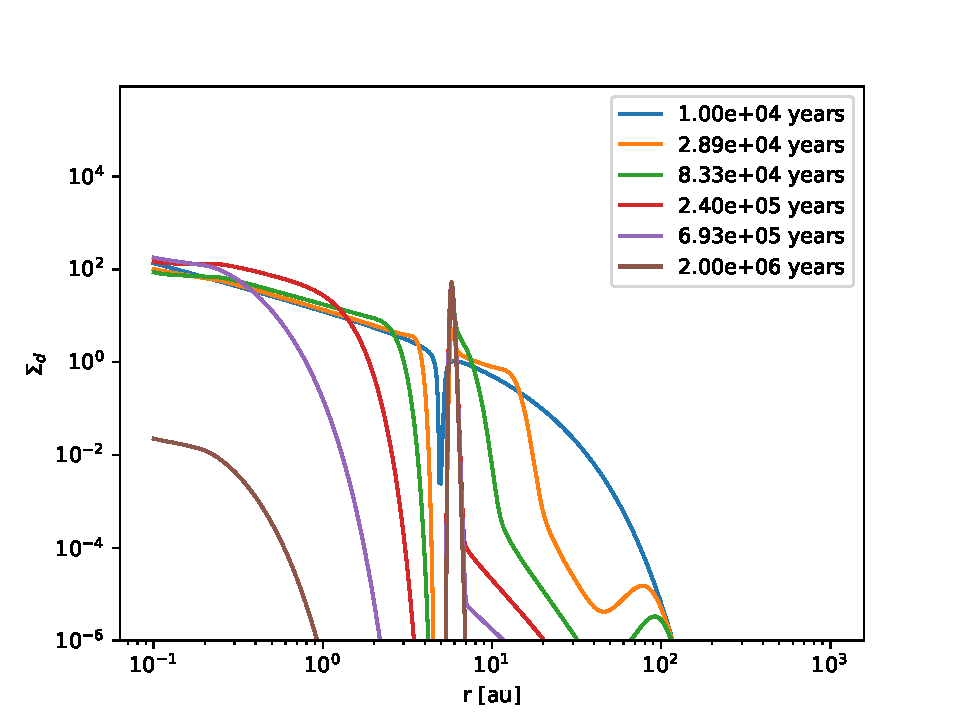
\includegraphics[width=0.7\textwidth]{../snippets/fig_snippet_planetgap_dustdrift_1_1.pdf}}
You see here that the dust rapidly drifts toward the planet gap in the outer disk.
There it gets trapped, as expected. The dust in the inner disk is drifting much
more slowly, because the Stokes number of these grains is much smaller there. The
model has a fixed grain size, so that the grains drift slower and slower as they
get further inward. They eventually just drift with the gas.

It is important to keep in mind that in this model the planetary gap is included
as a change in viscosity parameter $\alpha$. This means that the gas radial
velocity $v_r$ has a strong increase in the gap. This may drag along the
dust. Also, it would mean that the dust mixing coefficient is also increased, which
is not physical. To prevent this, the above listing creates a \code{self.alphamix}
as a copy of \code{self.alpha} {\em before} adding the planetary gap. The
dust drift/mixing method automatically checks if \code{self.alphamix} is present.
If yes, then it will use that value of $\alpha$ instead of the viscous $\alpha$,
for the computation of the mixing coefficient.

Here is another example. We now add two planets, we keep the Stokes number fixed
and tweak a few other parameters. In Python run it as:
\begin{codebox}
%run snippet_planetgap_dustdrift_2.py
\end{codebox}
Here is the listing:
\lstinputlisting{../snippets/snippet_planetgap_dustdrift_2.py}
\centerline{\includegraphics[width=0.7\textwidth]{../snippets/fig_snippet_planetgap_dustdrift_2_1.pdf}}
One can see the dust being trapped at both planetary gaps, and inside of the gaps
the dust disappears entirely. You can now use the technique of Section \ref{sec-simple-radtrans}
to make some radiative transfer maps for ALMA for instance.


\pagebreak
\section{Formation of a dead zone}
Let us make a simple example of a dead zone, but one that ``suddenly appears'':
we start from a normal disk, and set the $\alpha$ parameter to a low value within
a certain region. This is an unphysical starting condition, because the disk does
not suddenly get a dead zone, but it is what is often done in 2-D hydrodynamic disk
models, so let us see what the viscous evolution and dust drift say.

We set up a model with normal $\alpha=10^{-2}$, and deadzone
$\alpha_{\mathrm{dead}}=10^{-4}$ (i.e.\ not so ``dead'' as is often
assumed). The inner edge of the dead zone is taken at 0.4 au and the outer edge
at 5 au (both values are rather arbitrary).

The code snippet is
\code{snippet\_deadzone\_1.py}. In Python run it as:
\begin{codebox}
%run snippet_deadzone_1.py
\end{codebox}
Here is the listing:
\lstinputlisting{../snippets/snippet_deadzone_1.py}
\centerline{\includegraphics[width=0.5\textwidth]{../snippets/fig_snippet_deadzone_1_1.pdf}
  \includegraphics[width=0.5\textwidth]{../snippets/fig_snippet_deadzone_1_2.pdf}}
Note that we took 10$\times$ smaller time steps than in most other examples, to
ensure that the dust trapping behavior is properly modelled at the inner dead
zone edge. That means that the code is 10$\times$ slower in this example, but it
should not take more than a minute.

You can see a number of things in this example: At the start of the simulation
there is a sudden accumulation of gas mass at the outer edge of the dead zone.
This is to be expected, because there is continuous feeding of mass from the
outside, but the deadzone cannot transport this mass as quickly as it is fed.
Then this mass is slowly but gradually transported through the deadzone into
the inner disk. Eventually a (semi-)steady state is reached in which
$\Sigma_g\nu$ is (semi-)constant again, meaning that $\Sigma_g$ is higher in
the deadzone than outside by a factor of $\alpha/\alpha_{\mathrm{dead}}$.

Another interesting thing happens at the inner edge. There there is, initially,
also an accumulation of gas mass. This is because the viscously
active inner disk is transporting mass {\em outward} (as if it were a small
0.4 au size spreading disk). Only later does this bump disappear because
the system wants to achieve (semi-)steady state with $\Sigma_g\nu$ constant.

The dust also behaves interestingly. {\em Note that we took the Stokes number
  fixed to $\mathrm{St}=10^{-2}$. To ensure that the code does not accidently
  update $\mathrm{St}$ from the grain size at each time step and radius, we set
  \code{updatestokes=False}.} What happens is the following: Initially the dust
gets trapped at the outer deadzone edge because the gas bump is occurring
there. Meanwhile the dust in the deadzone itself is drifting inwards (see curves
at around $2.9\times 10^4$ and $8.3\times 10^4$ years). But as this gas bump is
spreading inward, the dust is released (around $2.4\times 10^5$ years) leading
to a sudden pile-up of dust at the inner edge of the dead zone (where there is
a long-lived bump).

Note that these results are for a relatively ``mild'' dead zone. If, however,
the $\alpha_{\mathrm{dead}}=10^{-6}$, the semi-steady state in the deadzone is
never reached. The code snippet
\code{snippet\_deadzone\_2.py} is the same as before, but only with
$\alpha_{\mathrm{dead}}=10^{-6}$. In Python run it as:
\begin{codebox}
%run snippet_deadzone_2.py
\end{codebox}
\centerline{\includegraphics[width=0.5\textwidth]{../snippets/fig_snippet_deadzone_2_1.pdf}
  \includegraphics[width=0.5\textwidth]{../snippets/fig_snippet_deadzone_2_2.pdf}}

Note that in both example models the deadzone edges are ultra-sharp. That is
unrealistic (if the above model is realistic in the first place). One may want
to smooth these edges.

Another, more physical way to implement the deadzone idea is to go back to the
original two-layered disk model of Gammie (1996) ApJ 457, 355. The {\sl DISKLAB}
package does not explicitly include a two-layered accretion model, but there is
a simply way to mimic this: by vertically averaging the $\alpha(r,z)$:
\begin{equation}
  \alpha(r) = \left\{
\begin{matrix}
  \alpha_1 & \qquad & (r<r_{\mathrm{in}}) \\
  \alpha_1 (\Sigma_{\mathrm{active}}/\Sigma_g)& \qquad & (\Sigma_g>\Sigma_{\mathrm{active}}) \\
  \alpha_1 & \qquad & (\Sigma_g\le \Sigma_{\mathrm{active}}) \\
\end{matrix}
  \right.
\end{equation}
where $\alpha_1$ is the normal active alpha value, $r_{\mathrm{in}}$ is the inner edge of
the dead zone (where we assume that the temperature of the disk is high enough
to thermally ionize alkali metals; we simply fix it here to the same value as the
inner deadzone edge radius as in the above examples).

The code snippet is
\code{snippet\_deadzone\_3.py}. In Python run it as:
\begin{codebox}
%run snippet_deadzone_3.py
\end{codebox}
Here is the listing:
\lstinputlisting{../snippets/snippet_deadzone_3.py}
\centerline{\includegraphics[width=0.5\textwidth]{../snippets/fig_snippet_deadzone_3_1.pdf}
  \includegraphics[width=0.5\textwidth]{../snippets/fig_snippet_deadzone_3_2.pdf}}
You can see that the deadzone rapidly shrinks as the disk evolves with time, and
has vanished entirely by the end of the simulation. This is
partly due to the high value of $\alpha_1=10^{-2}$.

If we put the $\alpha_1=10^{-3}$ then the disk evolves slower and the deadzone does
not vanish, but qualitatively the disk behaves much the same.

The code snippet is
\code{snippet\_deadzone\_4.py}. In Python run it as:
\begin{codebox}
%run snippet_deadzone_4.py
\end{codebox}
\centerline{\includegraphics[width=0.5\textwidth]{../snippets/fig_snippet_deadzone_4_1.pdf}
  \includegraphics[width=0.5\textwidth]{../snippets/fig_snippet_deadzone_4_2.pdf}}


%----------------------------------------------------------------------
%                     PART: VERTICAL STRUCTURE
%----------------------------------------------------------------------

\part{Disk Vertical Structure: 1+1D and 2-D}\label{part-vert-struct}

\chapter{Disk vertical structure}
\label{chap-vertical-structure}
The {\sf DISKLAB} code package also includes a model of the disk vertical
structure in a 1-D vertical manner. The \code{diskvertical} module is meant for
this. As usual, this is a class, called \code{DiskVerticalModel}, and it is entirely
{\em independent} of the \code{DiskRadialModel} class.

\section{Basic equations}\label{sec-disk-vert-struct-basic-eqs}
Let us make a simple 1-D vertical disk model at cylindrical radius $r_c$
distance from the star. The model has $z$ as the vertical coordinate, starting
from $z=0$ (midplane) to some value $z=z_{\mathrm{max}}$, which is typically a
few pressure scale heights. We have to make a distinction between {\em cylindrical}
radius $r_c$ and {\em spherical} radius $r_s$:
\begin{equation}
r_s^2 = r_c^2 + z^2
\end{equation}
For $z\ll r_c$ this distinction is usually so small that one can ignore
the difference. But if one is interested in the very upper layers of the
disk, especially at large radii from the star, the difference can become
large enough to be noticable.

\subsection{Hydrostatic equilibrium}\label{sec-vertical-hydrostatic-equil}
Strictly speaking, the hydrostatic equilibrium condition is a 3-D condition: The
force components in all three directions (in the corotating frame) have to add
up to zero. However, for axisymmetric disks without self-gravity, it fortunately
turns out that the pressure equilibrium in vertical direction (along cylinders)
becomes an independent 1-D ordinary differential equation in $z$. 

The gravitational force per unit mass of gas is
\begin{equation}\label{eq-force-grav}
{\bf f}_g = -\frac{GM_{*}}{r_s^3}\left(r_c{\bf e}_{r_c}+z{\bf e}_{z}\right)
\end{equation}
where ${\bf e}_{r_c}$ is the unit vector in cylindrical radial direction
and ${\bf e}_{z}$ the unit vector in vertical direction. The centrifugal force is
\begin{equation}\label{eq-force-cent}
{\bf f}_c = \frac{v_\phi^2}{r_c}{\bf e}_{r_c}
\end{equation}
and the pressure gradient force is
\begin{equation}\label{eq-force-pgrad}
  {\bf f}_p = - \frac{1}{\rho}\frac{\partial p}{\partial r_c}{\bf e}_{r_c}
  - \frac{1}{\rho}\frac{\partial p}{\partial z}{\bf e}_{z}
\end{equation}
where $p=\rho c_s^2$ is the gas pressure, and $c_s$ is the isothermal
sound speed (cf.~Eq.~\ref{eq-isothermal-sound-speed}). Hydrostatic equilibrium means
that all these forces add up to zero:
\begin{equation}
{\bf f}_g+{\bf f}_c+{\bf f}_p=0
\end{equation}
For the ${\bf e}_{z}$ component this leads to the equation
\begin{equation}\label{eq-vert-equil}
\frac{\partial \ln p(r_c,z)}{\partial z} = -\frac{GM_{*}}{(r_c^2+z^2)^{3/2}}\frac{z}{c_s(r_c,z)^2}
\end{equation}
If the temperature structure, and thus $c_s(r_c,z)$, is a {\em given} function
of $r_c$ and $z$ (see Subsection \ref{sec-vertical-temperature-structure}), then
Eq.~(\ref{eq-vert-equil}) can be directly numerically integrated from the
midplane upward, assuming we know the midplane pressure $p(r_c,0)$. This yields
the vertical pressure profile $p(r_c,z)$. By dividing this by the known
$c_s(r_c,z)^2$, we obtain the density profile $\rho(r_c,z)$ and the vertical
density structure has been found.

As promised, the 3-D hydrostatic structure equations have reduced to a simple
1-D ordinary differential equation (Eq.~\ref{eq-vert-equil}) that can be
integrated without knowledge of the density or pressure at other positions in
$r_c$ (or in azimuth). And this is not an approximation: it is exact. It works
because the right-hand-side of Eq.~(\ref{eq-vert-equil}) contains no dependence
on $\rho$ or $p$.

There is one small problem still, but that can be easily solved: Typically we do
not know $p(r_c,0)$ a-priori, but instead we prescribe the radial surface
density profile
\begin{equation}\label{eq-surfdens-def}
\Sigma(r_c) = \int_{-\infty}^{+\infty}\rho(r_c,z)dz
\end{equation}
So how do we find the vertical density profile that is consistent with this
(prescribed) surface density profile? The way we do this is as follows:
Numerically we start the vertical integration of Eq.~(\ref{eq-vert-equil}) with
a trial value of $p(r_c,0)$, integrate Eq.~(\ref{eq-vert-equil}), and rescale
$\rho(r_c,z)$ to match Eq.~(\ref{eq-surfdens-def}). This immediately gives us
the 2-D density structure.

Note that all of this does not work if we include self-gravity of the disk.

Let us now see how this works for the simplest example possible: a vertically
isothermal geometrically thin disk. Vertically isothermal means that
$c_s$ in Eq.~(\ref{eq-vert-equil}) can be considered a given constant. And
in the geometrically thin limit ($z\ll r_c$) we can approximately set
$r_s\simeq r_c$, or in Eq.~(\ref{eq-vert-equil}) set $r_c^2+z^2\simeq r_c^2$.
Under these simplifying conditions the solution to Eq.~(\ref{eq-vert-equil})
becomes:
\begin{equation}\label{eq-vertical-struct-gauss}
  \rho(r_c,z) = \frac{\Sigma_g(r_c)}{\sqrt{2\pi}\,H_p(r_c)}
  \exp\left(-\frac{1}{2}\frac{z^2}{H_p(r_c)^2}\right)
\end{equation}
with $H_p=c_s/\Omega_K$ and $\Omega_K=\sqrt{GM_{*}/r_c^3}$. This is the
Gaussian vertical density structure that implicitly stands at the basis
of the radial structure models of Part \ref{part-radial-disk} of this
tutorial (see e.g.~Equation \ref{eq-vertstr-gauss}).


\subsection{Vertical temperature structure}\label{sec-vertical-temperature-structure}
In Subsection \ref{sec-disk-vert-struct-basic-eqs} we assumed that we {\em know}
what the temperature structure $T(r_c,z)$ of the disk is. However, in general
this has to be calculated using a radiative transfer model.  And here we
encounter the issue of the 3-D geometry again, that we managed to circumvent in
Subsection \ref{sec-vertical-hydrostatic-equil}: The radiative transfer problem
in protoplanetary disks is a 3-D problem (or, with axial symmetry, at least a
2-D problem in the coordinates $r_c$ and $z$). The simplest way to see this is
to imagine how the light from the star (which irradiates and heats the disk) can
easily be shadowed by a vertically extended (``fat'') inner disk: in such a case
the stellar photons get absorbed by the disk regions close to the star (small
$r_c$) and never reach the surface of the disk regions far from the star (large
$r_c$). These outer disk regions will therefore be colder than if this shadowing
did not occur.

Strictly speaking, therefore, there is no accurate way to compute a 1-D vertical
structure model of the temperature of the disk without including the radial
structure as well (and thus making it a 2-D model). This will be dealt with
in Section \ref{sec-fld-rt-model} and Section \ref{sec-connect-radmc-3d}. 

However, as we have seen in Section \ref{sec-compute-tmid}, there are {\em
  approximate} methods to treat the radiative transfer as a local problem in
$r_c$, and thus making it a 1-D problem in $z$. This is what we will do here.

We will start with a simple estimate of the vertical density structure
$\rho(z)$. Let us assume that the stellar irradiation enters the disk under an angle
$\varphi$ called the {\em flaring angle}, which in the code is called
\code{flang}. The optical depth of the disk to the stellar radiation at a given
$z$ is then
\begin{equation}
\tau_{*}(z) = \int_z^\infty \frac{\rho_{\mathrm{d}}(z')\kappa_{\mathrm{P*}}}{\varphi}dz'
\end{equation}
where the dust density $\rho_{\mathrm{d}}$ is the dust density. For now, let us
assume that it is a given fraction of the gas density:
\begin{equation}
\rho_{\mathrm{d}} = \mathrm{dtg}\,\rho_{\mathrm{g}}
\end{equation}
where $\mathrm{dtg}$ is the dust-to-gas ratio, here assumed to be constant with
$z$. The opacity $\kappa_{\mathrm{P*}}$ is the {\em Planck mean opacity} for
stellar wavelengths, which for now we will assume to be a given value, but later
we will show how this can be self-consistently computed. We now can compute the
flux of stellar radiation:
\begin{equation}\label{eq-irrad-flux-flang}
F_{*}(z) = \frac{L_{*}}{4\pi r^2}\,e^{-\tau_{*}(z)}
\end{equation}
We do not take into account the stellar spectrum for now, just the
frequency-integrated stellar flux. The mean intensity of stellar radiation
at each height $z$ in the disk is then
\begin{equation}
J_{*}(z) = \frac{F_{*}(z)}{4\pi}
\end{equation}
The flux is extincted by the dust in the disk. We assume, for now, that the
albedo of the dust is zero, so that all the radiation of the star is absorbed
and re-emitted. The source term of this re-emission in units of $\mathrm{erg}\,\mathrm{cm}^{-3}
\,\mathrm{s}^{-1}$ is then
\begin{equation}
q_{*}(z) = \varphi\,\frac{dF_{*}(z)}{dz}
\end{equation}
One could also write $q_{*}(z)$ in terms of $J_{*}(z)$ and the extinction coefficient,
but we chose the flux-conservative form for numerical accuracy even at low numerical
resolution.

Next we handle the diffuse radiation field given by the mean intensity $J_{\mathrm{diff}}(z)$
and first moment $H_{\mathrm{diff}}(z)$. They obey the equations:
\begin{eqnarray}
  \frac{dH_{\mathrm{diff}}(z)}{dz} &=&  \frac{q(z)}{4\pi} \label{eq-1d-mom1}\\
  \frac{dJ_{\mathrm{diff}}(z)}{dz} &=&  -3\rho_{\mathrm{d}}(z)\kappa_{\mathrm{R}}H_{\mathrm{diff}}(z) \label{eq-1d-mom0}
\end{eqnarray}
where $\kappa_{\mathrm{R}}$ is the {\em Rosseland mean opacity} of the dust, and
$q(z)$ is the source term, which for an irradiation-only model is
$q(z)=q_{*}(z)$. Any viscous heating or other source terms can be included in
$q(z)$ as well by simple addition.  The boundary conditions are
$H_{\mathrm{diff}}(0)=0$ and
$H_{\mathrm{diff}}(z_{\mathrm{max}})=J_{\mathrm{diff}}(z_{\mathrm{max}})/\sqrt{3}$. Given
$q_{*}(z)$ we first integrate $H_{\mathrm{diff}}(z)$ from $z=0$ to
$z=z_{\mathrm{max}}$, starting with $H_{\mathrm{diff}}(0)=0$. Then we impose the
upper boundary condition, giving us $J_{\mathrm{diff}}(z_{\mathrm{max}})$, and
we integrate $J_{\mathrm{diff}}(z)$ back to the midplane.

Once we have the radiation field, we can compute the gas and dust temperature (which we
assume to be the same) according to:
\begin{equation}\label{eq-t-afo-jmean}
T(z) = \left(\frac{\pi}{\sigma_{\mathrm{SB}}}\big(J_{\mathrm{diff}}(z)+\frac{\kappa_{\mathrm{P*}}}{\kappa_{\mathrm{P}}(T)}J_{*}(z)\big)\right)^{1/4}
\end{equation}
where, as usual, $\sigma_{\mathrm{SB}}$ is the Stefan-Boltzmann constant and
$\kappa_{\mathrm{P}}(T)$ is the Planck-mean opacity of the dust for the
temperature $T$.

Once we have this vertical temperature profile, we can solve for the vertical
density profile using the equation of hydrostatic equilibrium, as described in
Section \ref{sec-vertical-hydrostatic-equil}. This will give a new density
profile, and thus the radiative transfer would have to be recomputed. In
practice this requires a few iterations until convergence is reached. We then
have the full vertical density and temperature solution.

\section{Basic setup}\label{sec-vertstruct-basic}
Let us set up a simple vertically isothermal disk model at $r_c=1\,\mathrm{au}$
to begin with. We fix the value of $\varphi$ and estimate the temperature to be
$T=(\tfrac{1}{2}\varphi L_{*}/4\pi r^2\sigma_{\mathrm{SB}})^{0.25}$.  The code
snippet is \code{snippet\_vertstruct\_basic\_1.py}. In Python run it as:
\begin{codebox}
%run snippet_vertstruct_basic_1.py
\end{codebox}
Here is the listing: \lstinputlisting{../snippets/snippet_vertstruct_basic_1.py}
\centerline{\includegraphics[width=0.5\textwidth]{../snippets/fig_snippet_vertstruct_basic_1_1.pdf}
  \includegraphics[width=0.5\textwidth]{../snippets/fig_snippet_vertstruct_basic_1_2.pdf}}
As you can see, the temperature is constant, as we assumed. The density profile
is accordingly almost a perfect Gaussian
(cf.~Eq.~\ref{eq-vertical-struct-gauss}). The slight deviation from Gaussian is
due to the difference between the cylindrical radius $r_c$ and spherical radius
$r_c$, as discussed in Section \ref{sec-vertical-hydrostatic-equil}. This difference
becomes larger for larger $z/r$. Since the ratio $H_p/r_c$ (the dimensionless
pressure scale height) increases with $r_c$, this difference becomes more relevant
at larger $r_c$, i.e.\ in the outer regions of the disk ($\sim 100\,\mathrm{au}$). 

Next let us compute the radiative transfer for this Gaussian vertical density profile.
The code snippet is
\code{snippet\_vertstruct\_basic\_2.py}. In Python run it as:
\begin{codebox}
%run snippet_vertstruct_basic_2.py
\end{codebox}
Here is the listing:
\lstinputlisting{../snippets/snippet_vertstruct_basic_2.py}
\centerline{\includegraphics[width=0.5\textwidth]{../snippets/fig_snippet_vertstruct_basic_2_1.pdf}
  \includegraphics[width=0.5\textwidth]{../snippets/fig_snippet_vertstruct_basic_2_2.pdf}}
The density profile is still a Gaussian, because we have not yet iterated on the vertical
hydrostatic equilibrium. But the temperature profile now clearly shows a transition from
midplane tempearture to (warmer) surface layer temperature, as expected.

Now let us feed this temperature profile back into the hydrostatic equilibrium equation and
do a few iterations. The code snippet is
\code{snippet\_vertstruct\_basic\_3.py}. In Python run it as:
\begin{codebox}
%run snippet_vertstruct_basic_3.py
\end{codebox}
Here is the listing:
\lstinputlisting{../snippets/snippet_vertstruct_basic_3.py}
\centerline{\includegraphics[width=0.5\textwidth]{../snippets/fig_snippet_vertstruct_basic_3_1.pdf}
  \includegraphics[width=0.5\textwidth]{../snippets/fig_snippet_vertstruct_basic_3_2.pdf}}

In practice you do not have to do this iteration by hand. There is a method for that.
The code snippet is
\code{snippet\_vertstruct\_basic\_4.py}. In Python run it as:
\begin{codebox}
%run snippet_vertstruct_basic_4.py
\end{codebox}
Here is the listing:
\lstinputlisting{../snippets/snippet_vertstruct_basic_4.py}
\centerline{\includegraphics[width=0.5\textwidth]{../snippets/fig_snippet_vertstruct_basic_4_1.pdf}
  \includegraphics[width=0.5\textwidth]{../snippets/fig_snippet_vertstruct_basic_4_2.pdf}}

\section{Including viscous heating}
We can include viscous heating using the following formula:
\begin{equation}
q_{\mathrm{visc}}(z) = \frac{9}{4}\Omega_K^2\rho_{\mathrm{gas}}(z)\nu(z)
\end{equation}
with viscosity $\nu$ given by
\begin{equation}
\nu(z) = \alpha(z) \frac{c_s(z)^2}{\Omega_K}
\end{equation}
This source is simply added to the irradiative source, so that the total source
is
\begin{equation}
q(z) = q_{\mathrm{visc}}(z) + q_{\mathrm{*}}(z)
\end{equation}

Let us simply add this to our example: we set $\alpha=10^{-3}$ and see what comes out.
The code snippet is\\
\code{snippet\_vertstruct\_vischeat\_1.py}. In Python run it as:
\begin{codebox}
%run snippet_vertstruct_vischeat_1.py
\end{codebox}
Here is the listing:
\lstinputlisting{../snippets/snippet_vertstruct_vischeat_1.py}
\centerline{\includegraphics[width=0.5\textwidth]{../snippets/fig_snippet_vertstruct_vischeat_1_1.pdf}
  \includegraphics[width=0.5\textwidth]{../snippets/fig_snippet_vertstruct_vischeat_1_2.pdf}}

{\sf DISKLAB} allows $\alpha$ to be $z-$dependent. So if the disk has a dead
zone, this will be included. Let us include such a ``dead zone'' in a simplified way:
we simply set $\alpha=0$ for $z<0.03\,r$. The code snippet is
\code{snippet\_vertstruct\_vischeat\_2.py}. In Python run it as:
\begin{codebox}
%run snippet_vertstruct_vischeat_2.py
\end{codebox}
Here is the listing:
\lstinputlisting{../snippets/snippet_vertstruct_vischeat_2.py}
\centerline{\includegraphics[width=0.5\textwidth]{../snippets/fig_snippet_vertstruct_vischeat_2_1.pdf}
  \includegraphics[width=0.5\textwidth]{../snippets/fig_snippet_vertstruct_vischeat_2_2.pdf}}

\section{Including 1-D vertical self-gravity}
\label{sec-selfgrav1d-vertical}
Self-gravity is a global force, and it is not really possible to treat it in a
localized 1-D vertical manner. But one can approximate the effect of the
vertical squeezing of the disk by its own gravity by employing the 1-D
plane-parallel approximation of the Poisson equation. If we have an infinite
plane surface with mass surface density $\Sigma$, then the vertical downward
gravitational body force of a particle above that plane is $f_z=-2\pi G\Sigma$.
We can now regard our 1-D vertical structure model as a set of 1-D infinite
planes. The body force at any given height $z$ is then
\begin{equation}
f_z(z) = - 4\pi G \int_0^z \rho(z)dz
\end{equation}
The factor 2 comes in because every step downward in $z$-direction means that a
plane of gas no longer attracts downward, but in fact pulls upward. At the midplane
the up- and down-ward forces cancel exactly, as they should. And for $z\infty$ the
force becomes $-2\pi G\Sigma$ as it should. 

Now we add this force to the vertical component of the gravitational force by
the star, and we can thus compute the self-gravity-corrected vertical structure.
This is all automatically handled by the
\code{diskvertical.iterate\_vertical\_structure()} method, with the keyword
\code{iterate\_selfgrav1d=True}.

The code snippet is
\code{snippet\_vertstruct\_selfgrav1d\_1.py}. In Python run it as:
\begin{codebox}
%run snippet_vertstruct_selfgrav1d_1.py
\end{codebox}
\centerline{\includegraphics[width=0.5\textwidth]{../snippets/fig_snippet_vertstruct_selfgrav1d_1_1.pdf}}

One sees that the self-gravity squeezes the vertical structure a bit, but not
much. Already the example above is not far from gravitational instability (it
has $Q\simeq 4$). If the surface density is chosen such that $Q\lesssim 2$, then
the disk would become gravitationally unstable, and the solution is not physical.

{\bf Warning:} Whenever you include self-gravity, you must always check that
the Toomre $Q>2$, otherwise you obtain a solution that, in reality, does not
exist because it is gravitationally unstable!
  
\section{Using more realistic opacities}

{\bf IN PROGRESS}

\section{Time-dependent radiative transfer}
Although the radiation field itself propagates with the speed of light, and is
thus effectively instant, the reaction of the gas temperature to the radiative
cooling takes a certain amount of time. To implement this we follow Kuiper,
Klahr, Dullemond, Kley \& Henning (2010), A\&A 511, 81. In this method the local
gas and dust temperature is assumed to be always in strict equilibrium with the
radiation field according to Eq.~(\ref{eq-t-afo-jmean}). The time-dependent
zeroth moment equation of the radiation field now includes the thermal energy of
the gas and the dust. We assume that the thermal heat capacity of the dust is
negligible compared to that of the gas. The energy conservation equation
then reads
\begin{equation}\label{eq-timedep-rt-ener-eq}
  \frac{\partial(E_{\mathrm{gas}}(z)+E_{\mathrm{diff}}(z))}{\partial t}
  = -\frac{\partial F_{\mathrm{diff}}(z)}{\partial z} + q(z)
\end{equation}
where $E_{\mathrm{diff}}=4\pi J_{\mathrm{diff}}/c$, $F_{\mathrm{diff}}=4\pi
H_{\mathrm{diff}}$ and $E_{\mathrm{gas}}=c_{\mathrm{v}}\rho_{\mathrm{gas}}T$,
where $c_{\mathrm{v}}$ is the specific heat of the gas, given by
\begin{equation}
c_{\mathrm{v}}=\frac{k_B}{(\gamma-1)\mu m_p}
\end{equation}
Since the gas temperature is assumed to be strictly coupled to the
radiation field, we can express $\partial_t E_{\mathrm{gas}}$ in terms of
$\partial_t E_{\mathrm{rad}}$ through
\begin{equation}\label{eq-timederiv-of-egas-in-ediff}
  \frac{\partial E_{\mathrm{gas}}}{\partial t} = c_{\mathrm{v}}\rho_{\mathrm{g}}\frac{\partial T}{\partial t}
  =\frac{c_{\mathrm{v}}\rho_{\mathrm{g}}}{4aT^3}\frac{\partial E_{\mathrm{diff}}}{\partial t}
\end{equation}
where we used the following version of Eq.~(\ref{eq-t-afo-jmean}):
\begin{equation}
aT^4 = E_{\mathrm{diff}} + \frac{\kappa_{\mathrm{P*}}}{\kappa_{\mathrm{P}}(T)}E_{*}
\end{equation}
with $a=4\sigma_{\mathrm{SB}}/c$. {\em For now we ignore the time-derivative of
  $\kappa_{\mathrm{P}}(T)$}, so that Eq.~(\ref{eq-timederiv-of-egas-in-ediff})
follows directly. Now eleminating $E_{\mathrm{gas}}$ in Eq.~(\ref{eq-timedep-rt-ener-eq})
in favor of $E_{\mathrm{diff}}$, we obtain
\begin{equation}
\left(1+\frac{c_{\mathrm{v}}\rho_{\mathrm{g}}}{4aT^3}\right)
  \frac{\partial E_{\mathrm{diff}}(z)}{\partial t}
  = -\frac{\partial F_{\mathrm{diff}}(z)}{\partial z} + q(z)
\end{equation}
This is the 1-D form of the equation 6 from Kuiper et al., who define
$f_c=1/(1+c_{\mathrm{v}}\rho_{\mathrm{g}}/4aT^3)$ to simplify their equation.

In {\sf DISKLAB} we
use $J_{\mathrm{diff}}=cE_{\mathrm{diff}}/4\pi$ and
$H_{\mathrm{diff}}=F_{\mathrm{diff}}/4\pi$. So the equation then becomes
\begin{equation}\label{eq-timedep-diffuse-rt}
\frac{1}{c}\left(1+\frac{c_{\mathrm{v}}\rho_{\mathrm{g}}}{4aT^3}\right)
  \frac{\partial J_{\mathrm{diff}}(z)}{\partial t}
  = -\frac{\partial H_{\mathrm{diff}}(z)}{\partial z} + \frac{q(z)}{4\pi}
\end{equation}
We now integrate Eq.~(\ref{eq-timedep-diffuse-rt}) using an implicit integration
scheme, using the diffusion solver of appendix
\ref{sec-standard-diff-eq-solver-onedee}. Since that solver does not have an
explicit factor before the time-derivative, we simply provide the solver with a
space-dependent time step $\Delta
t(z)=dt/c(1+c_{\mathrm{v}}\rho_{\mathrm{g}}(z)/4aT(z)^3)$.

Now let us experiment with this. We start with an irradiated disk with
$\varphi=0.05$ in full equilibrium. Now we change the flaring angle to
$\varphi=0.07$, and let the time-dependent radiative diffusion change the
temperature. We take a single time step of 100 years.

The code snippet is
\code{snippet\_vertstruct\_timedep\_1.py}. In Python run it as:
\begin{codebox}
%run snippet_vertstruct_timedep_1.py
\end{codebox}
Here is the listing:
\lstinputlisting{../snippets/snippet_vertstruct_timedep_1.py}
\centerline{\includegraphics[width=0.7\textwidth]{../snippets/fig_snippet_vertstruct_timedep_1_1.pdf}}

As you can see the radiative heating takes time to penetrate into the disk. This is
the time-dependent heating from the top. To convince yourself that everything is
self-consistent, you can (as a test) change \code{flang1} to the same value as
\code{flang} (i.e.~0.05). In that case nothing should happen, and you can convince
yourself that that is indeed the case.

Note that we took {\em a single time step} here, for a non-linear problem. That
is of course not quite correct. We should do multiple smaller time steps, because
the factor $f_c$ changes in time.

Note also that we {\em did not change the density structure} during this time
step. So the disk has not reacted to the change in temperature. This is, of
course, not self-consistent.

We should let the disk accomodate hydrostatically to the new temperature. But in
doing so, we have to do this {\em adiabatically}. In other words, we have to fix the
{\em specific entropy} everywhere, and then find a new hydrostatic equilibrium.
The adiabatic equation of state is
\begin{equation}
p_{\mathrm{gas}}(z) \equiv \rho_{\mathrm{gas}}(z)\frac{k_B T(z)}{\mu m_p} = K(z) \rho_{\mathrm{gas}}(z)^\gamma
\end{equation}
The specific entropy is
\begin{equation}
s = s_0 + \frac{k_B}{\mu(\gamma-1)}\ln K
\end{equation}
where we take $s_0=0$. For each gas packet the $s$ should (upon re-computation of
the vertical hydrostatic structure $\rho_{\mathrm{gas}}(z)$) remain the same
{\em in a comoving Lagrangian manner}. So we first map $s(z)$ onto $s(\sigma)$,
where $\sigma(z)$ is the column density:
\begin{equation}
\sigma(z) = \int_z^\infty \rho(z)dz
\end{equation}
with the property $\sigma(0)=\Sigma_{\mathrm{gas}}/2$. We then
compute the new $\rho_{\mathrm{gas}}(z)$ for the given temperature structure
$T(z)$ and recompute the new $\sigma_{\mathrm{new}}(z)$. We now map $s(\sigma)$
onto this new $\sigma_{\mathrm{new}}(z)$ through interpolation (linear interpolation
is usually enough). This gives a new function $s(z)$ from which we can compute
a new temperature $T(z)$. It is important to define the $\sigma(z)$ as the column
density toward $z=+\infty$ instead of between $z=0$ and $z$, because in the very
surface layers the density is so low that one would hit the machine precision limit
if $\sigma(z)$ is defined from the bottom. The interpolation would then go wrong.

Let us try this method out. The code snippet is
\code{snippet\_vertstruct\_timedep\_2.py}. In Python run it as:
\begin{codebox}
%run snippet_vertstruct_timedep_2.py
\end{codebox}
Here is the listing:
\lstinputlisting{../snippets/snippet_vertstruct_timedep_2.py}
\centerline{\includegraphics[width=0.7\textwidth]{../snippets/fig_snippet_vertstruct_timedep_2_1.pdf}}

One sees that due to the higher temperature, the surface of the disk has expanded a
bit, hence the red curve is moving upward again near the surface layers.

What is peculiar is the sudden upward trend of the temperature at the upper
edge. This is because due to the expansion of the disk, while keeping the
$z_{\mathrm{max}}$ fixed, the {\em very} upper layers just below the
$z_{\mathrm{max}}$ have, so to speak, left the upper grid boundary. Although we have
renormlized the total density (and therefore no mass is really lost), the effect
is that the mapping of the entropy onto the new $\sigma$-grid is thus slightly wrong
near the upper boundary. This is a computational / numerical effect caused by
imposing a fixed upper grid boundary at $z=z_{\mathrm{max}}$. When we do another
time step with the time-dependent radiative diffusion, this disappears, but it
will always re-appear after calling the hydrostatic adiabatic solver. If the
time steps are small enough it should be not a major problem, however. It
occurs at such a high location in the surface layers, that the denisty there
is negligbly low.

The solution is simple: just do a tiny time step for radiative transfer and
things are back in equilibrium.

The code snippet is
\code{snippet\_vertstruct\_timedep\_3.py}. In Python run it as:
\begin{codebox}
%run snippet_vertstruct_timedep_3.py
\end{codebox}
Here is the listing:
\lstinputlisting{../snippets/snippet_vertstruct_timedep_3.py}
\centerline{\includegraphics[width=0.7\textwidth]{../snippets/fig_snippet_vertstruct_timedep_3_1.pdf}}


\section{Dust settling and vertical mixing}
The \code{dustvertstruct.py} module also allows for modeling the vertical
settling and vertical mixing of dust species (or of gas chemical species, which
are mathematically equivalent to dust with zero stopping time). Each dust or gas
species is represented by an object of type \code{diskvertcomponent}, in much
the same way as the radial \code{DiskRadialModel} object can be supplemented with
\code{DiskRadialComponent} objects (see Section \ref{sec-multi-dust-spec}).  A
\code{diskvertcomponent} object should be linked to an existing
\code{DiskVerticalModel} object, again in the same way as a \code{DiskRadialComponent} is
linked to a \code{DiskRadialModel} object (see Chapter \ref{chap-dust-drift-mixing}).

The modeling of the vertical settling and mixing goes in a very similar
way as for the radial drift and mixing of Chapter \ref{chap-dust-drift-mixing}.

Here is an example. The code snippet is
\code{snippet\_vertstruct\_dustsett\_1.py}. In Python run it as:
\begin{codebox}
%run snippet_vertstruct_dustsett_1.py
\end{codebox}
Here is the listing:
\lstinputlisting{../snippets/snippet_vertstruct_dustsett_1.py}
\centerline{\includegraphics[width=0.7\textwidth]{../snippets/fig_snippet_vertstruct_dustsett_1_1.pdf}}

Note that this snippet demonstrates both the time-dependent modeling of the
dust settling (using the function \code{timestep\_settling\_mixing()}),
as well as the computation of the steady-state solution
(using the function \code{compute\_settling\_mixing\_equilibrium()}).

\section{Effect of dust weight on vertical structure}
In most cases we can compute the vertical pressure balance solution without
having to worry about the weight of the dust. The reason is that it is generally
the case that the dust-to-gas ratio is much smaller than unity. However, there
could be instances where radial trapping of dust leads to such a strong
accumultation of dust at a given radius, that the vertically integrated
dust-to-gas ratio becomes close to unity. In that case, the weight of the dust
will have a non-negligible effect on the vertical pressure equilibrium of the
disk. Essentially the gas pressure will not only have to support the weight of
the gas, but also that of the dust. For the same disk temperature, the disk will
then become a bit flatter.

The vertical pressure balance equation given by Eq.~(\ref{eq-vert-equil}) then
becomes
\begin{equation}\label{eq-vert-equil-dustload}
  \frac{\partial \ln p(r_c,z)}{\partial z} = -\left(1+
  \frac{\rho_{\mathrm{d}}(r_c,z)}{\rho_{\mathrm{g}}(r_c,z)}\right)
  \frac{GM_{*}}{(r_c^2+z^2)^{3/2}}\frac{z}{c_s(r_c,z)^2}
\end{equation}
where $\rho_{\mathrm{d}}$ is the volume density of all dust species together,
while $\rho_{\mathrm{g}}$ is the volume density of the gas. Note that once
$\rho_{\mathrm{d}}>\rho_{\mathrm{g}}$ we should expect the streaming instability
to operate (Youdin \& Goodman, 2005, ApJ 620, 459). And when
$\rho_{\mathrm{d}}\ll\rho_{\mathrm{g}}$ the effect of dust-loading is negligible.
So the applicability of Eq.~(\ref{eq-vert-equil-dustload}) is limited in
scope. But here is a snippet to model it:
\begin{codebox}
%run snippet_vertstruct_dustload_1.py
\end{codebox}
Here is the listing:
\lstinputlisting{../snippets/snippet_vertstruct_dustload_1.py}
\centerline{\includegraphics[width=0.7\textwidth]{../snippets/fig_snippet_vertstruct_dustload_1_1.pdf}}

One can see that the dust-laden gas is a bit more (though not much) concentrated
toward the midplane. 

\newpage

\chapter{Disk 2D structure}
\label{chap-2d-structure}
Now that we dealt with the 1-D radial disk structure and the 1-D vertical disk
structure, it is time to combine them into a 2-D disk structure. This is done
with the \code{Disk2D} class. The simplest version of a 2-D model is simply a
sequence (i.e.\ a python list) of 1-D vertical structure models, one for each
radial grid point of a 1-D radial disk model. This is called a 1+1D model. The
vertical structure models are then independent of each other. They ``do not
feel'' their neigbors.  Such a model is therefore not really a true 2-D model,
but it often serves its purpose.

The \code{Disk2D} class also contains methods for truly 2-D models, where the
vertical slices do communicate, e.g.\ via radiation or via self-gravity. These
truly 2-D models require truly 2-D arrays, instead of a list of 1-D vertical
models. The \code{Disk2D} class contains methods for mapping the 1+1D ``list of
vertical structures'' to truy 2-D arrays, and backward.

Another issue is that some methods of the \code{Disk2D} class require the
disk model to be in {\em spherical} coordinates. The 1-D vertical structure
models are truly vertical, i.e.\ they are along cylindrical coordinate lines.
The \code{Disk2D} class contains coordinate mappings from cylindrical to
spherical coordinates, and back.

Here is a summary of the three different representations of 2-D models:
\begin{itemize}
\item {\em 1+1D List of vertical structures:}\\
  \parbox{0.6\textwidth}{This is the simplest extension of the vertical structure models of
  Chapter \ref{chap-vertical-structure}. It is simply a python list of
  1-D vertical structure models of the type discussed in 
  Chapter \ref{chap-vertical-structure}. One starts with a 1-D {\em radial}
  model, and for each radial grid point one constructs a 1-D vertical model
  and adds it to the list called \code{Disk2D.verts}. So
  \code{Disk2D.verts[3]} is the 1-D vertical structure model at radius
  \code{Disk2D.r[3]}.}
  \parbox{0.4\textwidth}{\centerline{\includegraphics[width=0.3\textwidth]{disklab_grid_1p1d.pdf}}}
  \newpage
\item {\em 2-D Cylindrical coordinates:}\\
  \parbox{0.6\textwidth}{This is the 2-D version of the 1+1D List of vertical structures.
  You can use \code{Disk2D.convert\_1p1d\_to\_cyl2d()} to map the 
  1+1D List of vertical structures onto the 2-D cylindrical coordinates.
  The $z$-grid points are $r$-dependent, such that for radius \code{Disk2D.r[ir]}
  (with \code{ir} being the radial index, e.g.\ \code{ir=3} for the third
  radial grid point), the vertical grid \code{Disk2D.cyl2d\_zz[ir,:]} corresponds
  to the $z$-grid of vertical structure model \code{Disk2D.verts[ir]}.
  The physical quantities in the 2-D cylindrical model are thus a
  {\em direct copy} of the 1+1D model: no interpolation is needed. The only
  difference with the 1+1D model is that now all the data are available in
  a single 2-D array. For instance, the gas density is then
  \code{Disk2D.cyl2d\_rhogas[:,:]} instead of
  \code{Disk2D.verts[:].rhogas[:]}. Always keep in mind, though, that if
  you manipulate e.g.\ \code{Disk2D.cyl2d\_rhogas[:,:]}, then
  \code{Disk2D.verts[:].rhogas[:]} stays unaffected, until you call
  \code{Disk2D.convert\_cyl2d\_to\_1p1d()} to copy the data back.
  Also keep in mind that \code{Disk2D.convert\_cyl2d\_to\_1p1d()} does
  not copy everything. Please check out the code to see details.}
  \parbox{0.4\textwidth}{\centerline{\includegraphics[width=0.3\textwidth]{disklab_grid_cyl2d.pdf}}}
\item {\em 2-D Spherical coordinates:}\\
  \parbox{0.6\textwidth}{The 2-D spherical coodinates $(r_{\mathrm{sper}},\theta)$ are fundamentally
  different from the previous two. Instead of $z$ we have $\theta$ as the
  ``vertical'' coordinate, and ``vertical'' is now curved along the sphere. Very
  close to the equatorial plane the two coordinate systems become tangent, and
  thus for $z\ll r$ one can {\em approximately} say that
  $z/r\simeq\pi/2-\theta$. It is for this reason that for geometrically thin
  disks one can make a simplfied approximative mapping from cylindrical to
  spherical coordinates by simply ignoring the difference between the
  cylindrical radius $r$ and the spherical radius $r_{\mathrm{spher}}$, and
  by setting $z/r=\pi/2-\theta$. The advantage is that no interpolation is
  needed if the grid points in $z_{ij}$ are chosen linearly proportional to
  cylindrical radius $r_i$ (i.e.\ $z_{ij}/r_i=z_{0j}/r_0$), and the grid
  points in $\theta_j$ are chosen as $\pi/2-z_{0j}/r_{0}$. However, a proper
  mapping between cylindrical and spherical coordinates does require interpolation,
  since the 2-D gridpoints of the two coordinate systems do not match.
  The mapping between the coordinate systems is done with
  \code{Disk2D.coord\_trafo\_cyl2d\_to\_spher2d()} and
  \code{Disk2D.coord\_trafo\_spher2d\_to\_cyl2d()}. Note that for reasons
  related to the multi-D diffusion/Poisson solver, the spherical arrays
  are 3-D arrays, with the right index always 0.}
    \parbox{0.4\textwidth}{\centerline{\includegraphics[width=0.3\textwidth]{disklab_grid_spher2d.pdf}}}
\end{itemize}

\section{1+1D disk models}
The easiest way to make a 2D (radial-vertical) disk model is to simply make a
sequence of 1-D vertical disk models ``next to each other''. This is called a
1+1D model. This is made easy with the \code{Disk2D} class. The idea is to
first make a 1-D {\em radial} disk model with the \code{DiskRadialModel} class (see
Chapter \ref{chap-diskradialmodel-class}), and then make a \code{Disk2D} model
with it.

Here is an example. The code snippet is
\code{snippet\_vertstruct\_1p1d\_1.py}. In Python run it as:
\begin{codebox}
%run snippet_vertstruct_1p1d_1.py
\end{codebox}
Here is the listing:
\lstinputlisting{../snippets/snippet_vertstruct_1p1d_1.py}
\centerline{\includegraphics[width=0.5\textwidth]{../snippets/fig_snippet_vertstruct_1p1d_1_1.pdf}
\includegraphics[width=0.5\textwidth]{../snippets/fig_snippet_vertstruct_1p1d_1_2.pdf}}
%
These figures show the vertical 1-D models at 10 radii logarithmically spaced between
0.1 au and 200 au. One can clearly see that the disk has a flaring geometry and
that the disk at small $r$ is affected by viscous heating near the midplane.

However, when the other regions of the disk become very optically thin,
the 1+1D approach breaks down, and will give the wrong midplane temperature.
Below is an example of such a case. The code snippet is
\code{snippet\_vertstruct\_1p1d\_2.py}. In Python run it as:
\begin{codebox}
%run snippet_vertstruct_1p1d_2.py
\end{codebox}
Here is the listing:
\lstinputlisting{../snippets/snippet_vertstruct_1p1d_2.py}
\centerline{\includegraphics[width=0.5\textwidth]{../snippets/fig_snippet_vertstruct_1p1d_2_1.pdf}}
%
The key difference with the previous example is that we now have a
Lynden-Bell-Pringle-like exponential cut off of the outer disk. The
outer disk thus becomes optically thin. The midplane temperature is
then no longer correctly described by the 1+1D model. 


%{\bf [ADD MODEL WITH ITERATED FLIDX USING THE CHIANG \& GOLDREICH 2001 METHOD]}


\section{A note on the breakdown of 1+1D models at the inner rim}
\label{sec-dust-inner-rim}
%
A key point of 1-D flaring disk models, including their 1+1D extensions, is to
use the relatively flat geometry to simplify the radiative transfer of the
irradiating photons from the star. This simplification breaks down badly at the
``disk inner rim'', whether this be the true inner edge of the disk, or merely
the location where all the dust evaporates, or simply a place where the dust has
been removed by other processes (such as radial drift). The radiative transfer
at such an ``inner rim'' can no longer be approximated with a ``flaring angle
recipe''. It becomes truly 2-D/3-D. As long as you are not interested in the
regions close to such an ``inner rim'', the 1-D and 1+1D models are a reasonable
approximation. But near such ``inner rims'' full 2-D/3-D radiative transfer
becomes necessary. For this, see Section \ref{sec-fld-rt-model} and
Section \ref{sec-connect-radmc-3d}.


\section{Computing the true azimuthal velocity}
\label{sec-true-vphi}
%
In the simplest approximation we can assume that the azimuthal velocity $v_\phi$
equals the local Kepler velocity $v_K=\sqrt{GM_{*}/r}$. In Section
\ref{sec-compute-omega} we have, however, seen that in reality the $v_\phi$
slightly deviates from this Kepler velocity due to the radial pressure
gradient. In that Section we have studied this phenomenon only in the disk
midplane. Above the midplane, however, things become a bit more difficult.

In Section \ref{sec-vertical-hydrostatic-equil} we discussed the force balance,
decomposed in vertical and cylindrical-radial direction. We used only the
vertical component, in order to compute the vertical density structure.  To
obtain an expression for $v_\phi(r_c,z)$ we will now use the cylindrical-radial
component of the force balance. So, adding the ${\bf e}_{r_c}$ components of
Eqs.~(\ref{eq-force-grav}, \ref{eq-force-cent}, \ref{eq-force-pgrad}) together
and demanding this sum to be zero, we obtain
\begin{equation}\label{eq-vphi-full}
  v_\phi^2 = \frac{GM_{*}}{r_s^3}r_c^2 + c_s^2\left.\frac{\partial \ln p}{\partial \ln r_c}\right|_{z=const}
\end{equation}
The double-logarithmic pressure gradient is computed horizontally, keeping $z$
constant. We used $p=\rho c_s^2$ to obtain the above equation. If we
define
\begin{equation}\label{eq-vkep-with-z}
v_K(r_c,z) \equiv \sqrt{\frac{GM_{*}}{r_s^3}r_c^2}
\end{equation}
then we see that the pressure gradient term in Eq.~(\ref{eq-vphi-full})
represents, as expected, the deviation from Kepler. But we also see that the
Kepler velocity (Eq.~\ref{eq-vkep-with-z}) drops with height $z$, approximately
(for small $z$) with a factor $1-1.5\,(z/r_c)^2$. In practice the pressure
gradient will make the disk {\em sub-}kepler close to the midplane, but {\em
  super-}kepler well above the midplane. This is because, as a result of the
increase of the pressure scale height with radius ($dH_p/dr>0$), the radial
pressure gradient will become positive at large $z$, even if it is negative at
$z=0$. In other words: sufficiently above the midplane, the gas pressure
gradient pushes the gas {\em inward}, irrespective of whether the midplane
pressure gradient is negative or positive.

To numerically compute the radial pressure gradient we need a full 2-D or 1+1-D
disk model. We give here an example for the case of a vertically isothermal
disk. 
The code snippet is
\code{snippet\_vertstruct\_vphi\_1.py}. In Python run it as:
\begin{codebox}
%run snippet_vertstruct_vphi_1.py
\end{codebox}
Here is the listing:
\lstinputlisting{../snippets/snippet_vertstruct_vphi_1.py}
\centerline{\includegraphics[width=0.5\textwidth]{../snippets/fig_snippet_vertstruct_vphi_1_1.pdf}
\includegraphics[width=0.5\textwidth]{../snippets/fig_snippet_vertstruct_vphi_1_2.pdf}}
%
The left plot shows the $v_\phi$ (Eq.~\ref{eq-vphi-full}) as a function of $z/r_c$
at $r_c=47\,\mathrm{au}$, in units of the Kepler velocity at $z=0$. Overplotted
is the Kepler velocity without the pressure correction
(Eq.~\ref{eq-vkep-with-z}). At the midplane ($z/r_c=0$) one can see that the
disk rotates indeed with subkepler velocity, as expected due to the negative
radial pressure gradient. But well above the midplane the disk becomes
super-Keplerian. Overall the pressure gradient has the effect of making
$v_\phi(z)$ dropping less fast with $z$ than $v_K(z)$. In the figure we also
overplot the analytic solution of $v_{\phi}(z)$ according to Eq.~(13) of
Nelson, Gressel \& Umurhan (2013) MNRAS 435, 2610.

The right plot shows contour lines of the angular frequency $\Omega(r_c,z)$
(solid lines), the specific angular momentum $l(r_c,z)=\Omega r_c^2$ (dashed lines),
and the kinetic energy $e_{\mathrm{kin}}(r_c,z)=\Omega^2 r_c^2$ (dotted lines). The
contour lines are for midplane $v_\phi$ values of 2.5, 3.0 and 3.5 km/s. This
figure shows that above the midplane the contour lines diverge as a result of the
vertical shear.

We know, however, that disks are not vertically isothermal. So let us redo the
above computation of $v_\phi(z)$ but now for a disk which is irradiated from the
top according to a flaring angle of $\varphi = 0.05$ (see Section
\ref{sec-vertstruct-basic}).
The code snippet is
\code{snippet\_vertstruct\_vphi\_2.py}. In Python run it as:
\begin{codebox}
%run snippet_vertstruct_vphi_2.py
\end{codebox}
Here is the listing:
\lstinputlisting{../snippets/snippet_vertstruct_vphi_2.py}
\centerline{\includegraphics[width=0.7\textwidth]{../snippets/fig_snippet_vertstruct_vphi_2_1.pdf}}
One sees that the velocity becomes more strongly subkepler high above the
midplane. But the overall behavior remains the same as for the vertically
isothermal disk.

\section{1+1D disk models with 2-D approximate radiative transfer}
\label{sec-fld-rt-model}
%
The next level of realism is to replace the 1-D vertical radiative transfer with
2-D radiative transfer. Here we do this still in a simplified (and quick) way,
using the two-stage procedure described in Kuiper, Klahr, Dullemond, Kley \&
Henning (2010), A\&A 511, 81. The idea is to do the same two-stage procedure as
we did in in the 1-D vertical model of Section
\ref{sec-disk-vert-struct-basic-eqs} and following sections, but this time not
just in the 1-D vertical approximation but in 2-D axial symmetry. This elimiates
the need for the awkward guessing of the flaring angle or flaring index, and it
properly allows for radial radiative diffusion in the disk, which can be important
for the proper treatment of shadowed regions. One can also do stage 1 (irradiation)
in a 2-D way and still do stage 2 (diffusive radiative transfer) in a 1-D vertical
way. Strictly speaking one can also do the stage 1 in 1-D flaring angle approach
and stage 2 in 2-D axisymmetry, but it is not clear if that makes sense.

\subsection{2-D method for the irradiation (= stage 1)}
\label{sec-2d-irrad}
The direct irradiation of the disk by the star in a 2-D model is a matter of
ray-tracing along radial rays through the disk. The method
\code{radial\_raytrace()} does this in a simple way. This method requires that
the $z$-grids at the different radii are radially lined up: i.e.\ that the grid
points obey $z_i(r_1)/r_1=z_i(r_2)/r_2$, and that we assume that the star is a
point source.  Then the radial ray-tracing is simply integrating along
$z/r=\mathrm{const}$ lines, i.e.~at fixed vertical grid point. We therefore
define a new, and dimensionless, vertical coordinate
\begin{equation}
  \zeta = \frac{z}{r}
\end{equation}
The equation is then:
\begin{equation}
F_{*}(r,\zeta) = \frac{L_{*}}{4\pi r_{\mathrm{spher}}^2} e^{-\tau_{*}(r,\zeta)}
\end{equation}
where $r_{\mathrm{spher}}=\sqrt{r^2+z^2}$
(compare to Eq.~\ref{eq-irrad-flux-flang}), where $\tau_{*}(r,\zeta)$ is the
radial optical depth at stellar wavelengths
\begin{equation}
\tau_{*}(r,\zeta) = \sqrt{1+\zeta^2}\int_{R_{*}}^r \rho_{\mathrm{gas}}(r',\zeta)\kappa_{*} dr'
\end{equation}
Here the $\sqrt{1+\zeta^2}$ factor accounts for the fact that
$r_{\mathrm{spher}}=\sqrt{r^2+z^2}$, and that, in fact, we integrate along the spherical
$r_{\mathrm{spher}}$ instead of the cylindrical $r$.

Here is an example. We replace the radius-by-radius flaring-angle irradiation method
\code{irradiate\_with\_flaring\_index()} with the 2-D irradiation
method \code{radial\_raytrace()}. The code snippet is
\code{snippet\_vertstruct\_2d\_1.py}. In Python run it as:
\begin{codebox}
%run snippet_vertstruct_2d_1.py
\end{codebox}
Here is the listing:
\lstinputlisting{../snippets/snippet_vertstruct_2d_1.py}
\centerline{\includegraphics[width=0.5\textwidth]{../snippets/fig_snippet_vertstruct_2d_1_1.pdf}
\includegraphics[width=0.5\textwidth]{../snippets/fig_snippet_vertstruct_2d_1_2.pdf}}
%
Here we no not iterate the vertical hydrostatic structure. But the irradiation
is now done self-consistently. The diffuse radiation field is still done in a
1+1D manner, i.e.~thermal energy is still not exchanged between the radii.

Now let us iterate the vertical structure. The code snippet is
\code{snippet\_vertstruct\_2d\_2.py}. In Python run it as:
\begin{codebox}
%run snippet_vertstruct_2d_2.py
\end{codebox}
Here is the listing:
\lstinputlisting{../snippets/snippet_vertstruct_2d_2.py}
\centerline{\includegraphics[width=0.5\textwidth]{../snippets/fig_snippet_vertstruct_2d_2_1.pdf}
\includegraphics[width=0.5\textwidth]{../snippets/fig_snippet_vertstruct_2d_2_2.pdf}}
%
Here the vertical structure is iterated 10 times. We see here a strange effect: the
middle of the disk appears to become dark and cold. This is a shadowing effect. The
inner disk is vertically too extended, casting a shadow over the middle part of the
disk, which accordingly cools and vertically shrinks, exacerbating the shadowing
effect. Is this realistic? One problem is that since the diffuse radiative transfer
is still done in a 1+1D manner, the diffuse radiation field cannot transport any
energy radially through the disk. A shadow is thus {\em absolute}. In reality, the
diffuse radiation field may, however, counteract too strong shadows by ``leaking''
energy from the illuminated parts of the disk into the shadowed part of the disk.
To incorporate this, we need to also replace the 1+1D diffuse radiative transfer
with a true 2-D diffuse radiative transfer, which is the topic of the next subsection.

\subsection{2-D method for the diffusive radiative transfer (= stage 2)}
In Section \ref{sec-disk-vert-struct-basic-eqs} we gave the 1-D equations for
the diffuse radiation transfer step (Eqs.~\ref{eq-1d-mom1}, \ref{eq-1d-mom0}).
Now we wish to replace this with the true 2-D diffusion equation:
\begin{equation}
\vec\nabla \cdot \vec H
\end{equation}
with
\begin{equation}
\vec H = -\frac{f}{3\rho_{\mathrm{d}}\kappa_{\mathrm{Ross}}} \vec\nabla J
\end{equation}
where $f$ is a factor that, for perfect diffusion theory, is $f=1$, but for
Flux-Limited-Diffusion (FLD) is $f=\lambda/3$ with $\lambda$ being the
flux limited from Levermore \& Pomraning (1981).

The most natural coordinate system to solve the FLD equations is the spherical
coordinate system. This is what {\sf DISKLAB} does. However, the 1+1D disk model
is a series of 1-D vertical structure models that are, by assumption, perfectly
vertical. In other words: the 1+1D model is in cylindrical coordinates. So we
need to perform a coordinate mapping from cylindrical to spherical coordinates
before we solve the FLD equations, and then back to map the result back to the
1+1D model.

For very geometrically thin disks the difference between cylindrical coordinates
$(r,z)$ and spherical coordinates $(r_{\mathrm{spher}},\theta)$ is tiny. In
principle one could, without major error, simply use the same grid for
$r_{\mathrm{spher}}$ as for $r$, and simply map each 1-D vertical model to a
spherical shell, with $\theta$ grid equal to $\theta\simeq\pi/2-z/r$. That is
the simplest ``coordinate transformation'' from cylindrical to spherical, where
no interpolation is necessary. The only tricky bit is that the indexing order
of $\theta$ goes from pole to equator, while $z/r$ goes from equator upward.
In Python this is simply done with indexing \code{[::-1]}. This method of
approximate transformation between cylindrical and spherical coordinates is
called the {\em thin-disk approximation}.

However, the proper way is to do a true coordinate transformation between
cylindrical and spherical coordinates (and back), which requires a mapping of
the physical variables such as density and temperature from one coordinate
system to the other. This requires interpolation. In the \code{disk2d} module of
{\sf DISKLAB} this is done using the
\code{disk2d.coord\_trafo\_cyl2d\_to\_spher2d()} and
\code{disk2d.coord\_trafo\_spher2d\_to\_cyl2d()} functions.

Although this full-fledged mapping back and forth between the cylindrical and
spherical coordinates is formally better than using the thin-disk approximation,
it does have some numerical issues. Well above the midplane, there will be
regions of space covered by the spherical grid that are outside of the
cylindrical grid, and vice versa. A back-and-forth mapping will therefore
introduce strong boundary effects if not handled carefully. In the FLD method
these boundary effects are taken care of by employing our knowledge of the
optically thin solution. 

Now let us get to business. We use the irradiation computation from Section
\ref{sec-2d-irrad}. Then we set up a spherical coordinate system. We map the
relevant quantities to the spherical coodinates. Then we call the FLD
solver. The result is then mapped back to the 1+1D model. Most of this
stuff is handled by \code{disk2d.solve\_2d\_rad\_diffusion()}. You can
switch to the simplified thin-disk approximation by setting
\code{simplecoordtrans=True} in that function. By default it is set to
\code{False} (i.e.\ by default the true coordinate mapping is used).

The code snippet is
\code{snippet\_vertstruct\_2d\_3.py}. In Python run it as:
\begin{codebox}
%run snippet_vertstruct_2d_3.py
\end{codebox}
Here is the listing:
\lstinputlisting{../snippets/snippet_vertstruct_2d_3.py}
\centerline{\includegraphics[width=0.5\textwidth]{../snippets/fig_snippet_vertstruct_2d_3_1.pdf}
\includegraphics[width=0.5\textwidth]{../snippets/fig_snippet_vertstruct_2d_3_2.pdf}}

This method can also be iterated with vertical hydrostatic equilibrium.
The code snippet is
\code{snippet\_vertstruct\_2d\_4.py}. In Python run it as:
\begin{codebox}
%run snippet_vertstruct_2d_4.py
\end{codebox}


\section{Self-gravity of the disk in 2D}
\label{sec-selfgravity-2d}
If a disk mass is not small compared to the stellar mass, the effect of self-gravity
kicks in. In extreme cases it can lead to the gravitational instability, in which
case {\sf DISKLAB} can not be used, because that is a time-dependent phenomenon,
and likely also non-axisymmetric.

However, at disk masses below instability (i.e.\ Toomre Parameter $Q>2$),
self-gravity can still affect the structure of the disk, even though it does not
destabilize it.  A stable self-gravitating disk will be slightly flatter, and it
will have a different Keplerian rotation curve than a non-self-gravitating disk.

The \code{Disk2D} class has a method \code{Disk2D.solve\_2d\_selfgrav()} that
computes the self-gravity forces in 2-D.  Internally it uses 2-D spherical
coodinates, but it initially performs a transformation from 1+1D to 2-D
cylindrical, and then to 2-D spherical coordinates.  The key input to the
Poisson solver is then the density \code{Disk2D.spher\_rho[:,:,0]}. It then
solves the Poisson equation, obtaining the potential in 2-D spherical
coordinates (\code{Disk2D.spher\_pot[:,:,0]}). This is then mapped back
onto the 2-D cylindrical coordinates \code{Disk2D.cyl2d\_pot[:,:]}, and
the gradients of this potential are then numerically evaluated at the
cell walls: \code{Disk2D.cyl2d\_gradpot\_r[:,:]} for the cylindrically
radial gradient and \code{Disk2D.cyl2d\_gradpot\_z[:,:]} for the vertical
gradient. The negative of these gradients are then the bodyforces belonging
to the potential.

Typically it is prudent to set up a spherical grid that is radially extended
well beyond the grid of the cylindrical coordinates. Also the $\theta$-grid has
to be extended all the way to (close to) the pole.  This is because gravity is a
long-range force, and the boundary conditions we impose on the gravitational
potential are simple: we set $\vec n\cdot \nabla \Phi=0$ on both boundaries in
$\theta$ as wel as the inner boundary in $r_{\mathrm{spher}}$, and we set
$\Phi=0$ at the outer boundary in $r_{\mathrm{spher}}$. In particular the latter
is only (approximately) correct if the $\max(r_{\mathrm{spher}})$ is very far
out, i.e.\ much larger than the disk radius.

Here is an example of the computation of the self-gravity forces for a
given density distribution. The code snippet is
\code{snippet\_selfgrav2d\_1.py}. In Python run it as:
\begin{codebox}
%run snippet_selfgrav2d_1.py
\end{codebox}
It will spawn a set of wireframe surface plots to show the $(^{10}\log(r),z/r)$
dependence of the gravitational potential $\Phi$, and the two components of the
bodyforce $f_r$ and $f_z$. It will also plot the radial run of the gravitational
potential at different $\theta$ angle, and compare it to the potential
for when the mass would be a point source at the center. As expected:
the potential for the real 2-D distribution asymptotically matches the
potential for a point source of the same mass for large $r$. Here is a subset
of these plots:

\centerline{
  \includegraphics[width=0.5\textwidth]{../snippets/fig_snippet_selfgrav2d_1_1.pdf}
  \includegraphics[width=0.5\textwidth]{../snippets/fig_snippet_selfgrav2d_1_2.pdf}}

\centerline{
  \includegraphics[width=0.75\textwidth]{../snippets/fig_snippet_selfgrav2d_1_4.pdf}}

The snippet \code{snippet\_selfgrav\_2.py} has the same setup, but now makes
a global iteration to get the disk in vertical hydrostatic balance with the
self-gravity. 
\begin{codebox}
%run snippet_selfgrav2d_2.py
\end{codebox}
It plots the vertical structure at $r=14.7\,\mathrm{au}$, in the same
manner as shown in Section \ref{sec-selfgrav1d-vertical}, but now for
the full global self-gravity. 


\newpage


\chapter{Connecting to external code packages}
\label{chap-links-to-external-codes}

\section{Connecting to the radiative transfer code {\sf RADMC-3D}}
\label{sec-connect-radmc-3d}

{\bf [TODO]}

\section{Connecting to the dust evolution code {\sf ????}}

{\bf [TODO]}

\section{Connecting to the hydrodynamics code {\sf FARGO-3D}}

{\bf [TODO]}


\appendix
\chapter{Standard diffusion equation solver in 1-D}
\label{sec-standard-diff-eq-solver-onedee}
Here we describe a general-purpose Python subroutine \code{solvediffonedee()}
for solving (or advancing in time) a diffusion equation of the type:
\begin{equation}\label{eq-standard-advection-diffusion}
  \frac{\partial y(x,t)}{\partial t} + \frac{\partial y(x,t)v(x)}{\partial x}
  - \frac{\partial}{\partial x}\left(D(x)g(x)
  \frac{\partial}{\partial x}\left(\frac{y(x,t)}{g(x)}\right)\right)=s(x)
\end{equation}
If a time step is provided, the equation is advanced in time {\em one time
  step}. Since the method is fully implicit, the subroutine is stable even for
large time steps, though it is more accurate when using many small ones than one
big one. If no time step is provided, the stationary case is solved
(i.e.~$\partial/\partial t\rightarrow 0$).

The boundary conditions are:
\begin{equation}
p\frac{dy}{dx} + qy = r
\end{equation}
(type 0) or
\begin{equation}
p\frac{d(y/g)}{dx} + q(y/g) = r
\end{equation}
(type 1). For each of the two boundaries (left and right) you specify a tuple
(p,q,r,type).

It is also possible to insert special ``internal conditions'' somewhere inside
the grid.

Example of a time {\em in}dependent boundary value problem:
\begin{codebox}
import numpy as np
import matplotlib.pyplot as plt
from solvediffonedee import *
nx  = 100
x   = np.linspace(0.,1.,nx)
y   = np.zeros(nx)
v   = np.zeros(nx)+0.5
d   = np.ones(nx)
g   = np.ones(nx)
s   = np.ones(nx)
bcl = (0,1,1,0)
bcr = (-1,0,1,0)
y   = solvediffonedee(x,y,v,d,g,s,bcl,bcr)
plt.plot(x,y)
plt.show()
\end{codebox}
which gives a slightly asymmetric inverted parabola. For time-dependent problems
you have to set the keyword \code{dt} to the length of the time step. Please
refer to the documentation string for more details, by typing
\code{solvediffonedee?} in the python prompt.

The \code{solvediffonedee()} function stands at the basis of many of the
capabilities of {\sf DISKLAB}. It allows the viscous disk equations to be
time-integrated without insanely small time steps, and it is therefore the
key ingredient for the speed of {\sf DISKLAB}.

\chapter{Opacities}
\label{app-opacities}

{\bf [MODIFY THIS CHAPTER TO THE NEW OPACITY ROUTINES]}

Dust opacities change with grain size and grain composition. To compute
your own dust opacity tables {\sf DISKLAB} provides you with a Mie code
that does this for you. The code is called \code{bhmie.py} and is the
Python version of the famous Bohren \& Huffman Mie code. It was translated
from the f77 code of Bruce Draine into Python. A wrapper routine was
created to make it easier to use: \code{makedustopac.py}.

Before you can make a dust opacity you have to download the corresponding
optical constants. You can get the tables from the Jena optical constants
database:

\url{http://www.astro.uni-jena.de/Laboratory/OCDB/index.html}

Here is an example of making the opacity table of a spherical dust grain of 10
$\mu\mathrm{m}$ radius using the \code{pyrmg70.lnk} datafile:

\url{http://www.astro.uni-jena.de/Laboratory/OCDB/data/silicate/amorph/pyrmg70.lnk}

for Pyroxene with 70\% magnesium and 30\% iron.

The code snippet is
in \code{snippet\_make\_dust\_opacity\_1.py}. In Python run it as:
\begin{codebox}
%run snippet_make_dust_opacity_1.py
\end{codebox}
Here is the listing:
\lstinputlisting{../snippets/snippet_make_dust_opacity_1.py}
\centerline{\includegraphics[width=0.7\textwidth]{../snippets/fig_snippet_make_dust_opacity_1_1.pdf}}

For details on how to compute Rosseland and Planck mean opacities,
see Section \ref{sec-incl-real-dust-opac}.

\chapter{Embedding your {\sf DISKLAB} model in an interactive widget}
Often it is a nuisance to have to re- and re-run a model by hand to
get a feeling for its behavior. It would be useful to be able to make
an {\em interactive} plot that changes automatically when you change
the parameters through a set of sliders (one slider per parameter).
The module \code{disklab/interactive\_plot.py} does that for you.

The main thing you have to do is to make a Python function that creates your
model for a given set of parameters. Let us call this function
\code{modulfunc()}. The function should return an array that you wish to
plot. The array is, for example, the surface density as a function of
radius. The radius is then an array of r-values that is given as an argument to
\code{modulfunc()}. So within \code{modulfunc()} is where you design your
model. You choose which parameters should have sliders, and what the possible
values of these parameters are (e.g.\ an array of 100 values between 3. and 8.,
meaning that the slider will slide between 3 and 8, and have 100-2 intermediate
values). You also determine exactly what the plot should look like, what the
labels, limits, scales, colors etc are. The widget \code{interactive\_plot()}
only replaces the values of the curve in the plot with the new ones after it
calls \code{modulfunc()}. In a manner of speaking, the only thing that
\code{interactive\_plot()} does is to bring your figure to life. The way that
this is done is that you hand \code{interactive\_plot()} the \code{axes} object
returned by \code{plt.plot()}, and hand it over to \code{interactive\_plot()}.
Whenever the ``plot'' button is clicked by the user, \code{interactive\_plot()}
will read the current values of the sliders, hand them over to
\code{modelfunc()}, which will compute the new data. Then these new data are
given to the \code{axes} objects belonging to the curve, which will then replot
it.

\code{interactive\_plot()} also allows to have multiple curves being ``brought
to life''. Just plot each of the curves you want to plot, hand over the
\code{axes} objects of these curves in a list to \code{interactive\_plot()}.
Your \code{modelfunc()} should now return a numpy array of two results, instead
of just the results for one curve.

It is easiest to simply look at an example.

The code snippet is
in \code{snippet\_widget\_1.py}. In Python run it as:
\begin{codebox}
%run snippet_widget_1.py
\end{codebox}
Here is the listing:
\lstinputlisting{../snippets/snippet_widget_1.py}

Here is what this widget looks like:\\
\centerline{\includegraphics[width=0.7\textwidth]{widget_example_1.png}}

You can do many things with the \code{disklab/interactive\_plot.py}
module. Several examples are in the documentation string. In fact,
\code{interactive\_plot.py} is a stand-alone code that can be used for any kind
of interactive plotting, not just for {\sf DISKLAB}. And within {\sf DISKLAB}
you can use it for any kind of plotting you may want, not just for plots as a
function of radial coordinate $r$. The philosophy is: just make a plot you want
to make, and store the \code{axes} objects from the curves you want to bring to
life into a list \code{axmodel}, and pass that to \code{interactive\_plot()}.
You can even make multiple plot panels using the \code{plt.subplots()}
function, and have them simultaneously linked to the sliders.

Here is a variant of the above example, where, this time, the thermal emission
is plotted on top of some ``observed data''. The code snippet is in
\code{snippet\_widget\_2.py}. In Python run it as:
\begin{codebox}
%run snippet_widget_2.py
\end{codebox}
\centerline{\includegraphics[width=0.7\textwidth]{widget_example_2.png}}



\end{document}
